\documentclass[11pt,b5paper]{book}

\usepackage{parskip}
\setlength{\parskip}{0.5em}
\setlength{\parindent}{1.5em}

\usepackage{longtable}
\usepackage{xcolor}
\usepackage{fontspec}
\setmainfont[
Path = fonts/,
UprightFont = TitilliumWeb-Regular.ttf,
BoldFont = TitilliumWeb-Bold.ttf,
ItalicFont = TitilliumWeb-Italic.ttf,
BoldItalicFont = TitilliumWeb-BoldItalic.ttf
]{TitilliumWeb}

\usepackage{pgfplots}
\usepgfplotslibrary{polar}
\pgfplotsset{compat=1.18}

\usepackage{tikz}
\usetikzlibrary{shapes.geometric,
    positioning, shapes, shapes.multipart, backgrounds, arrows.meta, calc, fit, trees, decorations.pathreplacing}

\usepackage{amsmath}

\usepackage{tabularx}
\usepackage[b5paper,inner=2.5cm,
  outer=2.0cm,
  top=2.5cm,
  bottom=2.5cm]{geometry}
\usepackage[colorlinks=true, linkcolor=black, citecolor=blue, urlcolor=blue]{hyperref}
\usepackage{graphicx}
\usepackage{xcolor}
\graphicspath{{../figures/}}
\usepackage{svg}

\usepackage{subcaption}

\usepackage{hyperref}
\usepackage{xurl}

\hyphenation{
  a-ka-de-mik
  a-na-li-sis
  a-na-lyst
  an-tar-wi-la-yah
  ap-pli-ca-tion
  a-pli-ka-si
  ar-chi-tec-ture
  ar-ti-cle
  ar-si-tek
  ba-gi-an
  ber-la-pis
  ber-ja-lan
  ber-kon-tri-bu-si
  bu-si-ness
  bib-li-o-gra-fi
  bi-ro-kra-tis
  di-gi-tal
  di-e-va-lu-a-si
  di-per-te-gas
  di-kum-pul-kan
  di-per-ba-i-ki
  di-per-ta-han-kan
  di-per-tang-gung-ja-wab-kan
  di-pub-li-ka-si-kan
  di-rep-li-ka-si
  di-se-pa-ka-ti
  di-se-der-ha-na-kan
  do-ku-men
  do-ku-men-ta-si
  elek-tro-nik
  en-ter-prise
  hi-e-rar-kis
  hi-po-te-tis
  in-do-ne-sia
  in-for-ma-tion
  in-ter-na-si-o-nal
  in-ter-face
  ke-bu-tuh-an
  ka-pa-bi-li-tas
  ke-ber-lan-jut-an
  ke-pa-tu-han
  ke-pen-ting-an
  ke-se-su-ai-an
  ke-sen-jang-an
  ke-ter-gan-tung-an
  ko-pe-ra-si
  ko-mu-ni-ka-si
  kon-sep-tu-al
  kon-fe-ren-si
  kon-sul-ta-si
  kon-teks
  la-yan-an
  li-te-ra-tur
  ling-kup
  ma-ka-lah
  ma-ha-sis-wa
  ma-na-je-ri-al
  ma-na-ger
  ma-nu-sia
  me-ma-ha-mi
  me-me-ta-kan
  mem-ba-ha-ya-kan
  mem-ban-tu
  mem-ban-ding-kan
  mem-ba-ngun
  mem-ba-yang-kan
  mem-be-da-kan
  mem-per-ce-pat
  mem-pre-sen-ta-si-kan
  mem-per-tim-bang-kan
  mem-per-ta-han-kan
  mem-va-li-da-si
  me-lain-kan
  me-la-lui
  me-naut-kan
  men-je-las-kan
  me-nem-pat-kan
  me-nye-di-a-kan
  me-nyu-sun
  me-re-spons
  meng-ha-sil-kan
  meng-hu-bung-kan
  me-nga-ba-i-kan
  me-nge-lom-pok-kan
  me-ngom-bi-na-si-kan
  me-ya-kin-kan
  me-ta-da-ta
  mo-der-ni-sa-si
  na-si-o-nal
  net-work
  of-fi-cer
  or-ga-ni-sa-si
  pa-ra-dig-ma
  pas-ca-sar-ja-na
  pe-lak-sa-na-an
  pe-lang-gan
  pe-lin-dung-an
  pe-lun-cur-an
  pem-ba-ya-ran
  pem-be-la-jar-an
  pe-mim-pin
  pe-mang-ku
  pe-ne-li-ti-an
  pe-ne-ri-ma-an
  pe-ngung-kit
  peng-em-bang
  pe-ngem-bang-an
  pe-nyi-ap-an
  pe-nu-li-san
  pe-nye-leng-ga-ra-an
  pe-nyu-su-nan
  per-ta-nya-an
  per-ja-la-nan
  pe-rang-kat
  per-ca-ka-pan
  per-tim-bang-an
  pin-jam
  plat-form
  pro-fe-si-o-nal
  pro-cess-ing
  pro-duct
  pro-gram-ming
  pus-ta-ka
  rea-lis-tis
  re-ko-men-da-si
  re-le-van
  re-gis-tra-tion
  re-gu-la-si
  ru-ang
  se-rupa
  se-sung-guh-nya
  sek-to-ral
  sim-pan
  ske-na-ri-o
  stan-dar
  stra-te-gi
  stra-te-gis
  stra-te-gy
  te-kno-lo-gi
  tech-no-lo-gy
  ter-do-ku-men-ta-si
  ter-hu-bung
  ter-stan-dar
  trans-ak-si
  trans-for-ma-si
  se-per-ti
}


\usepackage{listings}

\lstdefinelanguage{yaml}{
    basicstyle=\ttfamily\scriptsize,
    keywordstyle=\color{blue}\bfseries,
    commentstyle=\color{gray}\itshape,
    stringstyle=\color{red},
    showstringspaces=false,
    breaklines=true,
    frame=lines,
    numbers=left,
    numberstyle=\tiny\color{gray},
    backgroundcolor=\color{lightgray!10},
    tabsize=2,
    morecomment=[l]{\#},
    literate=
      *{-}{{{\color{blue}\bfseries-}}}1
       {:}{{{\color{blue}\bfseries:}}}1
}

\lstdefinelanguage{bash}{
    keywords={},
    basicstyle=\ttfamily\scriptsize,
    keywordstyle=\color{blue}\bfseries,
    sensitive=true,
    commentstyle=\color{gray},
    stringstyle=\color{red},
    numbers=left,
    numberstyle=\tiny\color{gray},
    breaklines=true,
    frame=lines,
    backgroundcolor=\color{lightgray!10},
    tabsize=2,
    comment=[l]{\#},
    showstringspaces=false
}

\newcommand{\authors}[1]{{\chapterauthor{#1}\addtocontents{toc}{#1\par}}}
\newcommand{\HUGE}{\fontsize{40}{48}\selectfont}

\renewcommand{\contentsname}{Daftar Isi}
\renewcommand{\chaptername}{Bab}
\renewcommand{\figurename}{Gambar}
\renewcommand{\tablename}{Tabel}

\definecolor{praditagreen}{RGB}{37, 113, 71}

\makeatletter
\newcommand{\chapterauthor}[1]{%
    {\parindent0pt\vspace*{-25pt}%
        \linespread{1.1}\large\scshape#1%
        \par\nobreak\vspace*{35pt}}
    \@afterheading%
}
\makeatother

\begin{document}

    \begin{titlepage}
\thispagestyle{empty}
\begin{tikzpicture}[remember picture, overlay]

  % --- Latar belakang: gambar gedung memenuhi seluruh halaman ---
  \node[anchor=center, inner sep=0pt, opacity=0.10] at (current page.center) {
    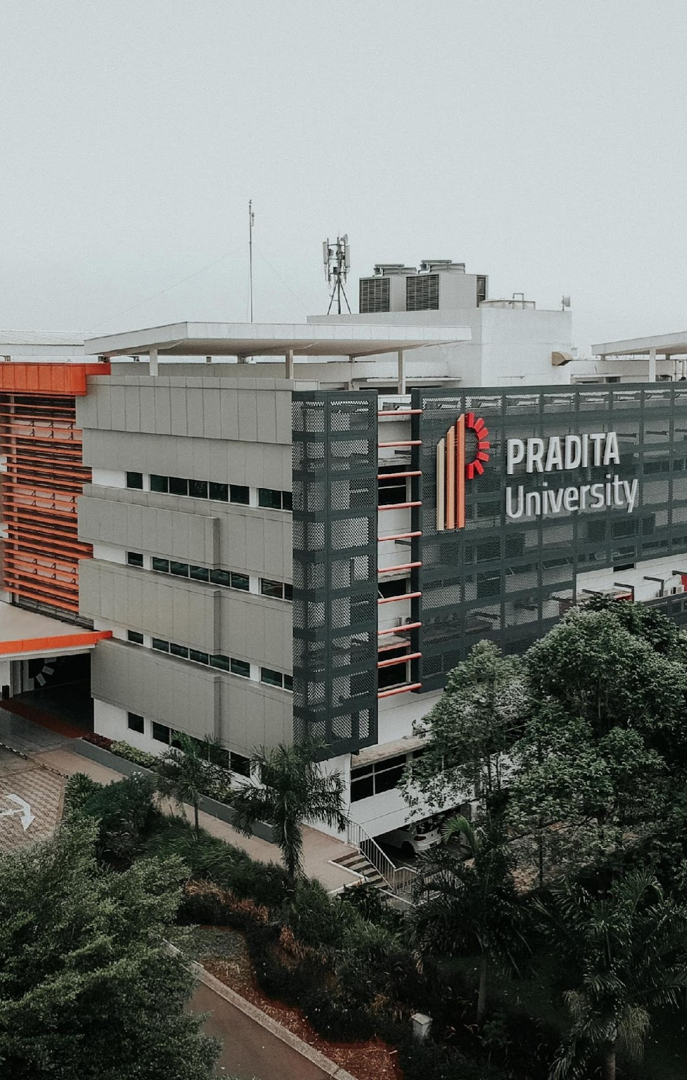
\includegraphics[width=\paperwidth, height=\paperheight, keepaspectratio=false]{../figures/building.png}
  };

  % --- Logo universitas: ditempatkan di tengah, dekat sisi atas ---
  \node[anchor=north, inner sep=0pt]
    at ([yshift=-0.10\paperheight] current page.north) {
    
\includegraphics[width=0.30\paperwidth]{../figures/logo_universitas.png}
  };

  % --- Blok judul: benar-benar di tengah halaman ---
  \node[anchor=center, align=center]
    at ([yshift=0.02\paperheight] current page.center) {
    \begin{minipage}{0.85\paperwidth}
      \centering
      {\LARGE \textbf{Modul Mata Kuliah IT30713}}\\[0.030\paperheight]
      {\HUGE \textcolor{praditagreen}{\textbf{Enterprise}}}\\[0.012\paperheight]
      {\HUGE \textcolor{praditagreen}{\textbf{\&}}}\\[0.012\paperheight]
      {\HUGE \textcolor{praditagreen}{\textbf{Platform Architecture}}}\\[0.050\paperheight]
      {\LARGE \textbf{Alfa Yohannis}}
    \end{minipage}
  };

  % --- Footer: pita hijau penuh selebar halaman, menempel di tepi bawah ---
  \node[
    anchor=south,
    fill=praditagreen,
    text=white,
    minimum width=\paperwidth,
    minimum height=0.13\paperheight,
    align=center,
    font=\Large\bfseries,
    inner sep=0pt
  ] at (current page.south) {%
    \begin{minipage}{0.9\paperwidth}
      \centering
      Program Studi Teknologi Informasi\\[4pt]
      Pradita University
    \end{minipage}%
  };

\end{tikzpicture}
\end{titlepage}


    \tableofcontents

    \chapter{Pendahuluan}

\section{Identitas Mata Kuliah}

Mata kuliah \textbf{IT30713 -- Enterprise \& Platform Architecture} merupakan
mata kuliah 3 SKS untuk mahasiswa magister di Pradita University. Mata kuliah
ini membahas cara \emph{Enterprise Architecture} (EA) membantu organisasi
menyelaraskan arah strategis dengan kapabilitas teknologi. Di dalamnya juga
dibahas peran strategi API dan tata kelola platform dalam membangun model
bisnis digital yang terhubung dengan ekosistem.

Mata kuliah ini dirancang untuk mahasiswa magister Indonesia yang sebagian
besar tidak berasal dari latar belakang IT. Karena itu, pembahasan diarahkan
pada cara berpikir strategis, manajerial, dan sistemik. Detail teknis tetap
diperkenalkan secukupnya, tetapi selalu ditempatkan sebagai alat bantu untuk
membuat keputusan, bukan sebagai tujuan utama pembelajaran.

\section{Capaian Pembelajaran}

\subsection{Capaian Pembelajaran Lulusan yang Didukung}

\begin{itemize}
    \item \textbf{CPL-4 -- System Design:} Mahasiswa menyusun artefak blueprint
    enterprise yang memetakan strategi, kapabilitas, data, aplikasi, teknologi,
    API, tata kelola, dan peta jalan sebagai dasar argumentasi makalah.
    \item \textbf{CPL-6 -- Leadership \& Collaboration:} Mahasiswa mengelola
    proyek penulisan individu, memberi dan menerima tinjauan sejawat, serta
    mengomunikasikan argumen rancangan kepada audiens teknis maupun non-teknis.
\end{itemize}

\subsection{Capaian Pembelajaran Mata Kuliah}

Setelah menyelesaikan mata kuliah ini, mahasiswa mampu:

\begin{enumerate}
    \item Menjelaskan peran Enterprise Architecture dalam transformasi digital
    organisasi.
    \item Menggunakan pendekatan TOGAF-lite untuk menyusun visi arsitektur,
    kondisi saat ini, arsitektur target, analisis kesenjangan, dan peta jalan.
    \item Memetakan domain Business, Data, Application, dan Technology (BDAT)
    sebagai dasar digital blueprint enterprise.
    \item Merancang strategi API untuk integrasi, kolaborasi, dan penciptaan
    nilai digital.
    \item Mengevaluasi model bisnis platform, network effects, ekosistem mitra,
    dan tata kelola platform.
    \item Merumuskan rekomendasi tata kelola, risiko, metrik, dan implikasi
    manajerial yang relevan untuk konteks Indonesia (UU PDP, UU ITE, OJK, BSSN,
    SNAP BI, PP 71/2019, Permenkominfo PSE).
    \item Menulis makalah ilmiah individual sesuai standar jurnal atau
    konferensi, termasuk struktur, sitasi, format, dan batas kemiripan naskah.
    \item Mempresentasikan makalah dalam format konferensi dan merespons umpan
    balik secara profesional.
\end{enumerate}

\section{Strategi Pembelajaran}

Pembelajaran menggunakan format \textbf{lokakarya individual}. Setiap sesi
berdurasi 3$\times$50 menit. Secara umum, 30 menit pertama digunakan untuk
pengantar konsep dan contoh kasus Indonesia, 90 menit berikutnya untuk
menyusun artefak atau bagian makalah secara individual, dan 30 menit terakhir
untuk konsultasi, tinjauan sejawat, serta refleksi kemajuan.

Setiap mahasiswa memilih satu organisasi studi kasus pada Sesi 1 dan
menggunakannya secara konsisten sampai akhir. Organisasi dapat berupa entitas
nyata atau hipotetis-realistis dalam konteks Indonesia, misalnya kampus, rumah
sakit, bank, koperasi atau BPR, retail, logistik UMKM, pemerintahan daerah,
agribisnis, atau BUMN. Istilah teknis dijelaskan melalui analogi manajerial dan
contoh organisasi.

\section{Luaran Utama dan Pelengkap}

\subsection{Luaran Utama}

Luaran utama mata kuliah adalah satu \textbf{makalah ilmiah individual} yang
diarahkan menjadi naskah siap diajukan setelah revisi final. Target publikasi
dapat berupa jurnal nasional terakreditasi (SINTA), jurnal internasional, atau
konferensi nasional/internasional yang relevan dengan Enterprise Architecture,
sistem informasi, transformasi digital, ekonomi API, atau strategi platform.

Seluruh aktivitas perkuliahan diarahkan untuk membangun bahan, kerangka,
argumen, artefak, dan kualitas akademik makalah secara bertahap, sesi demi
sesi.

\subsection{Luaran Pelengkap}

Luaran pelengkap wajib disusun sebagai bahan pembentuk makalah, tetapi tidak
memiliki bobot penilaian terpisah. Artefak ini berfungsi sebagai bukti analisis
dan bahan visual yang memperkuat makalah:

\begin{enumerate}
    \item Blueprint enterprise berbasis BDAT.
    \item Peta kapabilitas bisnis dan value stream.
    \item Visi arsitektur dan analisis pemangku kepentingan.
    \item Kondisi saat ini dan arsitektur target.
    \item Portofolio API atau peta kandidat API.
    \item Peta ekosistem platform atau kanvas model bisnis platform.
    \item Piagam tata kelola platform.
    \item Analisis kesenjangan dan peta jalan 12--24 bulan.
    \item Proposal makalah versi 1 (penanda kemajuan formatif pada Sesi 8).
    \item Bahan presentasi konferensi (Sesi 14).
    \item Surat pengantar atau daftar periksa pengajuan sesuai target publikasi.
\end{enumerate}

\section{Penilaian}

Penilaian akhir mata kuliah hanya berasal dari \textbf{makalah publikasi
individu} (100\%). Naskah harus dilengkapi artefak blueprint relevan sebagai
gambar, tabel, atau lampiran. Rincian rubrik disampaikan pada
Bab~\ref{ch:orientasi}. Rubrik tersebut menilai kejelasan masalah, kualitas
tinjauan pustaka, metode, kedalaman analisis, kualitas rancangan, diskusi dan
implikasi, kepekaan terhadap konteks Indonesia, kualitas akademik, serta
kelayakan publikasi.

Standar minimum naskah meliputi: mengikuti templat target publikasi, memiliki
minimal 15 referensi dengan setidaknya 5 referensi dari jurnal atau konferensi
terindeks, menggunakan gaya sitasi yang konsisten (APA, IEEE, atau gaya
target publikasi), menyertakan artefak blueprint yang benar-benar digunakan
dalam argumen, menjaga kemiripan Turnitin $\leq 25\%$ di luar daftar pustaka
dan kutipan wajar, serta mencantumkan keterangan penggunaan AI pada bagian
\emph{Acknowledgement} bila AI digunakan sebagai alat bantu.

\section{Rencana 14 Sesi Pembelajaran}

Tabel~\ref{tab:linimasa-sesi} menyajikan ikhtisar 14 sesi sekaligus linimasa
perkembangan makalah. Kolom \emph{Keluaran} menunjukkan hasil kerja mingguan
yang akan membentuk naskah final secara bertahap.

\begin{table}[htbp]
\centering
\scriptsize
\caption{Ikhtisar 14 sesi dan keluaran makalah per sesi.}
\label{tab:linimasa-sesi}
\begin{tabularx}{\textwidth}{@{}c X X@{}}
\hline
\textbf{Sesi} & \textbf{Topik} & \textbf{Keluaran untuk Makalah} \\
\hline
1  & Orientasi EA, Platform \& Penulisan Akademik & Pernyataan topik, kandidat target publikasi, motivasi awal \\
2  & Strategi Bisnis \& Rumusan Masalah & Rumusan masalah, pertanyaan penelitian (RQ), kontribusi awal \\
3  & TOGAF-lite, ADM \& Literature Review & Visi arsitektur, bibliografi awal ($\geq$10) \\
4  & Business Architecture & Peta kapabilitas, value stream, tinjauan pustaka v1 \\
5  & Data Architecture & Peta data konseptual, draf metode/pendekatan \\
6  & Application Architecture & Portofolio aplikasi, draf analisis \\
7  & Technology Architecture \& Kerangka Final & Arsitektur teknologi acuan, kerangka final \\
8  & Klinik Proposal Makalah (tengah semester) & \textbf{Proposal makalah v1} (penanda kemajuan formatif) \\
9  & API Strategy: API sebagai Produk & Draf analisis bagian strategi API \\
10 & API Design, Lifecycle \& Governance & Spesifikasi API, daftar periksa tata kelola \\
11 & Platform Economy \& Model Bisnis & Draf diskusi bagian platform \\
12 & Platform Governance, Etika \& Regulasi & Piagam tata kelola, draf diskusi dan kesimpulan \\
13 & Lokakarya Pra-Pengajuan & Draf final makalah, bahan presentasi, daftar periksa pengajuan \\
14 & Presentasi Konferensi \& Finalisasi & \textbf{Naskah final makalah ($100\%$)} \\
\hline
\end{tabularx}
\end{table}

\section{Aturan Tugas dan Etika Akademik}

\begin{enumerate}
    \item Seluruh tugas dikerjakan secara individu. Diskusi dan tinjauan
    sejawat diperbolehkan, tetapi naskah, analisis, dan kesimpulan harus
    merupakan karya masing-masing mahasiswa.
    \item Plagiarisme tidak diperkenankan. Kemiripan Turnitin $\leq 25\%$ di
    luar daftar pustaka dan kutipan wajar.
    \item AI boleh digunakan sebagai alat bantu untuk mencari ide awal,
    memperbaiki parafrase, atau memeriksa bahasa. Jika digunakan, mahasiswa
    wajib mencantumkan keterangannya pada bagian \emph{Acknowledgement}.
    Substansi analisis, argumen, dan kesimpulan tetap harus merupakan karya
    mahasiswa.
    \item Sitasi yang benar wajib untuk literatur, gambar, tabel, data, dan
    contoh kasus.
    \item Data sensitif organisasi dianonimkan atau digunakan dengan izin
    tertulis.
    \item Setiap rekomendasi dalam makalah memuat: alasan, dampak, risiko,
    prioritas, dan implikasi.
    \item Presentasi Sesi~14 wajib diikuti sebagai forum pertanggungjawaban
    akademik dan umpan balik final, namun nilai akhir tetap berasal dari
    makalah.
    \item Kehadiran minimal 75\%.
\end{enumerate}

\section{Catatan untuk Pembaca Mahasiswa}

Buku ini ditulis sebagai pendamping mata kuliah, bukan sebagai pengganti
literatur klasik di bidang Enterprise Architecture. Setiap bab dirancang agar
mahasiswa dapat membacanya secara mandiri sebelum pertemuan kelas, lalu
menggunakan sesi tatap muka untuk berlatih, berdiskusi, dan menerima umpan
balik.

Bahasa buku ini sengaja dibuat manajerial dan ringan. Jika menemukan istilah
teknis yang belum dikenal, pembaca dapat merujuk glosarium pada akhir setiap
bab atau membaca sumber tambahan yang tercantum pada bagian \emph{Bacaan
Lanjutan}.

Setiap bab diakhiri dengan latihan terapan individual yang menghasilkan
artefak atau narasi konkret. Artefak tersebut bukan tujuan akhir, melainkan
bahan penyusun yang akan dirangkai pada akhir semester menjadi satu makalah
publikasi yang utuh.

    \chapter{Orientasi: Enterprise Architecture, Platform, dan Penulisan Akademik}
\label{ch:orientasi}

\section*{Tujuan Pembelajaran}
\begin{itemize}
  \item Menjelaskan posisi \emph{Enterprise Architecture} (EA) sebagai jembatan
        antara strategi organisasi dan kapabilitas teknologi, dengan bahasa
        manajerial yang dapat dipahami audiens non-IT.
  \item Membedakan empat domain arsitektur enterprise---Business, Data,
        Application, Technology (BDAT)---serta peran API dan platform sebagai
        pengungkit nilai pada model bisnis digital modern.
  \item Mengenali anatomi makalah ilmiah yang relevan untuk bidang Enterprise
        Architecture dan platform/API, serta kriteria memilih target publikasi
        seperti jurnal SINTA, jurnal internasional, atau konferensi akademik.
  \item Menyusun pernyataan topik awal, memilih organisasi studi kasus dalam
        konteks Indonesia, dan merumuskan dua sampai tiga kandidat target
        publikasi sebagai dasar kerja satu semester.
\end{itemize}

\section{Pendahuluan}

Bab ini menjadi pintu masuk untuk seluruh perjalanan mata kuliah. Sebelum
memasuki konsep-konsep seperti TOGAF-lite, arsitektur BDAT, strategi API, dan
tata kelola platform, pembaca diperkenalkan terlebih dahulu pada
\emph{gambaran besar} yang mengikat semua konsep tersebut: bagaimana sebuah
organisasi menerjemahkan strategi menjadi keputusan arsitektur, dan bagaimana
mahasiswa magister non-IT dapat mengolah proses analisis itu menjadi makalah
ilmiah yang layak dipublikasikan.

Tiga gagasan utama bab ini saling berkaitan. Pertama, Enterprise Architecture
diperkenalkan bukan sebagai produk diagram yang rumit, melainkan sebagai cara
berpikir untuk membaca organisasi sebagai sebuah sistem. Kedua, ekonomi
platform dan strategi API diperkenalkan sebagai konteks bisnis modern yang
membuat keputusan arsitektur semakin strategis dan tidak lagi semata-mata
menjadi urusan tim TI. Ketiga, makalah publikasi diperkenalkan sebagai sarana
untuk mengubah proses analisis selama satu semester menjadi kontribusi
akademik yang dapat ditelaah oleh komunitas.

Bagi mahasiswa berlatar belakang non-IT, bab ini menegaskan bahwa keputusan
arsitektur enterprise pada dasarnya adalah keputusan manajerial yang dapat
dipahami melalui contoh bisnis sehari-hari. Bagi mahasiswa yang sudah pernah
bersentuhan dengan teknologi, bab ini menggeser perhatian dari kode dan
implementasi menuju pertanyaan yang lebih strategis: mengapa, untuk siapa,
dengan kompromi apa, dan berdasarkan bukti apa.

\section{Skenario Pembuka: Bank Daerah dan Rencana Transformasi Digital}

Bayangkan sebuah bank daerah di Indonesia, sebut saja \emph{Bank Wanua}, yang
selama tiga puluh tahun melayani nasabah lokal dengan jaringan cabang
tradisional. Direksi baru ingin membawa Bank Wanua masuk lebih serius ke
layanan digital: aplikasi mobile, integrasi pembayaran QRIS, kemitraan dengan
fintech,
serta layanan API publik untuk pelaku UMKM yang menjadi tulang punggung
ekonomi daerah. Dewan direksi sepakat tentang \emph{tujuan}, tetapi mereka
tidak yakin tentang \emph{urutan} dan \emph{prioritas}.

Direktur Operasional bertanya: ``Sistem mana yang harus diperbarui terlebih
dahulu, dan layanan mana yang sebaiknya dibuka sebagai API?'' Direktur
Kepatuhan bertanya: ``Bagaimana Bank Wanua memenuhi UU Perlindungan Data
Pribadi (UU PDP), Standar Nasional Open API Pembayaran (SNAP BI) Bank
Indonesia, dan ketentuan Otoritas Jasa Keuangan (OJK)?'' Direktur Pemasaran
bertanya: ``Apakah Bank Wanua sebaiknya menjadi platform mandiri atau
bergabung sebagai mitra ke ekosistem yang lebih besar?''

Tidak satu pun pertanyaan itu dapat dijawab hanya dengan keputusan teknis.
Setiap jawaban membutuhkan pemahaman tentang strategi bisnis, kapabilitas yang
sudah dimiliki, kondisi data dan aplikasi saat ini, aturan main regulasi
Indonesia, serta dinamika ekosistem mitra. Pertanyaan seperti inilah yang
menjadi wilayah kerja \emph{Enterprise Architecture}.

\subsection*{Pertanyaan Pemandu Bab Ini}

Sepanjang bab, lima pertanyaan berikut menjadi kompas pembaca:

\begin{enumerate}
  \item Apa sesungguhnya yang dimaksud dengan Enterprise Architecture, dan
        mengapa pembaca non-IT perlu memahaminya?
  \item Bagaimana platform dan API mengubah cara organisasi mengambil keputusan
        arsitektur dalam dekade terakhir?
  \item Apa yang membedakan sebuah \emph{makalah ilmiah} dari laporan proyek
        atau dokumen konsultasi?
  \item Bagaimana cara memilih target publikasi yang realistis dan relevan,
        khususnya dalam konteks Indonesia?
  \item Bagaimana pembaca dapat memulai perjalanan satu semester ini dengan
        memilih organisasi studi kasus dan topik makalah yang tepat?
\end{enumerate}

\section{Mengapa Topik Ini Penting bagi Pembaca Non-IT}

Mata kuliah ini sengaja dirancang untuk mahasiswa magister berlatar belakang
non-IT karena keputusan arsitektur enterprise pada akhirnya adalah keputusan
manajerial. Di dalamnya ada pertimbangan bisnis, anggaran, regulasi, sumber
daya manusia, budaya organisasi, dan risiko. Pengembang dan arsitek teknis
dapat membantu pelaksanaan, tetapi arah, prioritas, tata kelola, dan kompromi
yang diambil tetap perlu dipahami oleh pengambil keputusan.

Salah satu kesalahan yang sering terjadi adalah memperlakukan Enterprise
Architecture sebagai ``urusan tim TI''. Cara pandang ini membuat strategi
digital mudah gagal. Penyebabnya bukan selalu teknologi yang buruk, melainkan
keputusan teknis yang tidak tersambung dengan keputusan bisnis. Akibatnya,
organisasi dapat membayar mahal untuk sistem canggih yang jarang digunakan,
atau membangun kapabilitas TI yang tidak relevan dengan pelanggan dan model
bisnisnya.

Dengan memahami EA sebagai bahasa lintas fungsi, pembaca non-IT dapat menjadi
jembatan antara dewan direksi, tim bisnis, tim TI, dan mitra eksternal.
Kemampuan ini penting bagi peran strategis seperti Chief Information Officer,
Chief Digital Officer, Strategy Manager, Product Manager, Business Analyst,
atau pemimpin transformasi digital di sektor publik dan swasta.

\section{Kerangka Konseptual: Empat Pilar Bab Ini}

Empat konsep inti diperkenalkan pada bab pengantar ini:

\begin{enumerate}
  \item \textbf{Enterprise Architecture (EA)} sebagai jembatan strategi dan
        teknologi.
  \item \textbf{BDAT---Business, Data, Application, Technology} sebagai empat
        domain arsitektur yang akan dipetakan secara bertahap.
  \item \textbf{API dan Platform} sebagai pengungkit nilai pada model bisnis
        digital modern.
  \item \textbf{Anatomi Makalah Ilmiah} sebagai bentuk komunikasi akademik yang
        akan dibangun selama 14 sesi.
\end{enumerate}

\subsection{Enterprise Architecture: Jembatan Strategi dan Teknologi}

Enterprise Architecture adalah disiplin yang membantu organisasi menyelaraskan
strategi bisnis dengan kapabilitas teknologi melalui pemetaan, prinsip, dan
keputusan yang terdokumentasi. Hasil EA bukan sekadar kumpulan diagram,
melainkan keputusan terstruktur tentang apa yang perlu dipertahankan,
diperbaiki, diganti, atau dibangun dari awal.

Gambar~\ref{fig:ea-jembatan} menggambarkan posisi EA secara konseptual. EA
menjembatani \emph{lapisan strategi} (visi, model bisnis, dan tujuan
organisasi) dengan \emph{lapisan teknologi} (sistem, data, aplikasi, dan
infrastruktur). Tanpa jembatan ini, kedua sisi sering berbicara dengan bahasa
yang berbeda.

\begin{figure}[htbp]
\centering
\scalebox{0.95}{
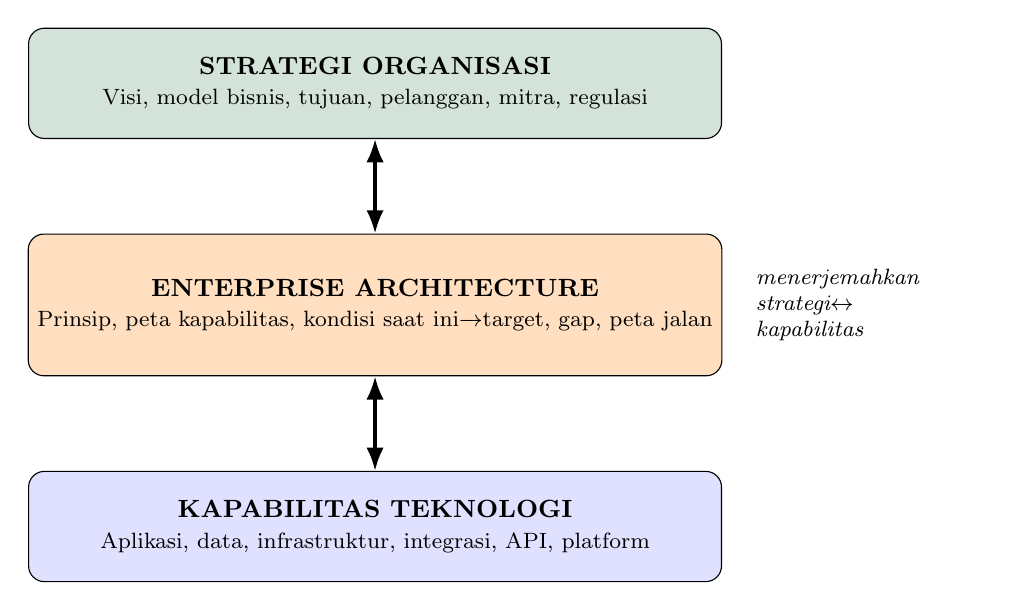
\begin{tikzpicture}[
  font=\small\bfseries,
  node distance=12mm,
  layer/.style={
    draw, rounded corners=2mm, align=center,
    minimum width=88mm, minimum height=14mm
  },
  strategi/.style={layer, fill=praditagreen!20},
  ea/.style={layer, fill=orange!25, minimum height=18mm},
  tek/.style={layer, fill=blue!12},
  arrow/.style={Latex-Latex, very thick}
]
\node[strategi] (s) {STRATEGI ORGANISASI\\
\footnotesize\mdseries Visi, model bisnis, tujuan, pelanggan, mitra, regulasi};
\node[ea, below=of s] (e) {ENTERPRISE ARCHITECTURE\\
\footnotesize\mdseries Prinsip, peta kapabilitas, kondisi saat ini$\to$target, gap, peta jalan};
\node[tek, below=of e] (t) {KAPABILITAS TEKNOLOGI\\
\footnotesize\mdseries Aplikasi, data, infrastruktur, integrasi, API, platform};

\draw[arrow] (s.south) -- (e.north);
\draw[arrow] (e.south) -- (t.north);

\node[right=0.3cm of e, align=left, font=\footnotesize\mdseries\itshape, text width=30mm]
 {menerjemahkan\\strategi$\leftrightarrow$\\ kapabilitas};
\end{tikzpicture}
}
\caption{Enterprise Architecture sebagai jembatan dua arah antara strategi
organisasi dan kapabilitas teknologi.}
\label{fig:ea-jembatan}
\end{figure}

Analogi yang dekat adalah cetak biru bangunan. Cetak biru bukanlah bangunan
itu sendiri; ia adalah gambar kerja yang membantu pemilik, kontraktor, pekerja
lapangan, dan pemeriksa berbicara tentang rancangan yang sama. Di dalamnya ada
pilihan tentang jumlah lantai, posisi tangga darurat, material pondasi, sistem
pendingin, urutan pembangunan, dan biaya. Cetak biru juga memuat asumsi dan
prinsip: apakah bangunan tahan gempa, hemat energi, dan ramah disabilitas.
Dengan cara serupa, Enterprise Architecture memuat keputusan dan prinsip
tentang ``bangunan organisasi'' yang sedang dirancang, dirawat, atau
ditransformasikan.

\subsection{BDAT: Empat Domain Arsitektur Enterprise}

Empat domain klasik dalam Enterprise Architecture, yang sering disingkat BDAT,
membantu kita memecah kerumitan organisasi menjadi beberapa lapisan yang lebih
mudah dibaca. Setiap lapisan dapat dianalisis secara terpisah, tetapi
keputusannya tetap saling memengaruhi. Gambar~\ref{fig:bdat-stack}
menunjukkan empat lapisan tersebut.

\begin{figure}[htbp]
\centering
\scalebox{0.95}{
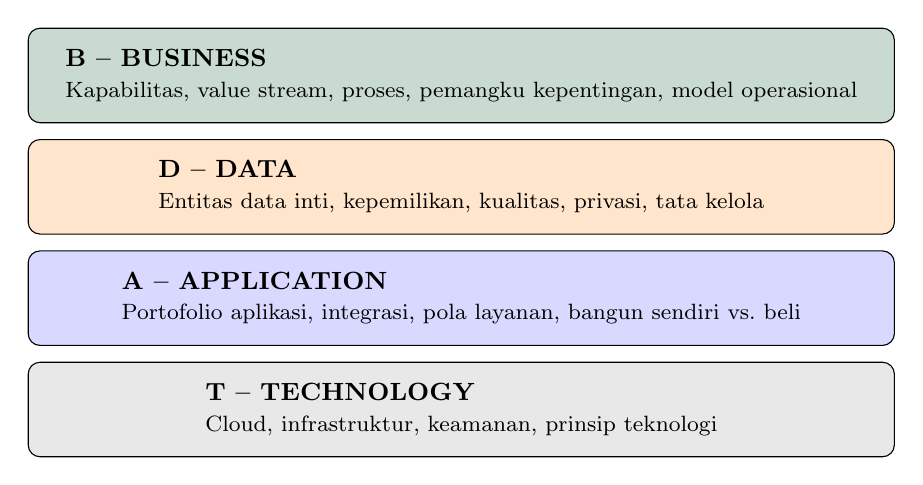
\begin{tikzpicture}[
  font=\small\bfseries,
  node distance=2mm,
  layer/.style={
    draw, rounded corners=1.5mm, align=left,
    minimum width=110mm, minimum height=12mm,
    inner xsep=4mm
  },
  business/.style={layer, fill=praditagreen!25},
  data/.style={layer, fill=orange!20},
  app/.style={layer, fill=blue!15},
  tech/.style={layer, fill=gray!18}
]
\node[business] (b) {\textbf{B} -- BUSINESS\\
\footnotesize\mdseries Kapabilitas, value stream, proses, pemangku kepentingan, model operasional};
\node[data, below=of b] (d) {\textbf{D} -- DATA\\
\footnotesize\mdseries Entitas data inti, kepemilikan, kualitas, privasi, tata kelola};
\node[app, below=of d] (a) {\textbf{A} -- APPLICATION\\
\footnotesize\mdseries Portofolio aplikasi, integrasi, pola layanan, bangun sendiri vs.\ beli};
\node[tech, below=of a] (t) {\textbf{T} -- TECHNOLOGY\\
\footnotesize\mdseries Cloud, infrastruktur, keamanan, prinsip teknologi};
\end{tikzpicture}
}
\caption{Empat domain arsitektur enterprise (BDAT) tersusun dari lapisan
strategi-bisnis di puncak hingga teknologi pendukung di dasar.}
\label{fig:bdat-stack}
\end{figure}

Domain \textbf{Business} menjawab pertanyaan: apa yang dilakukan organisasi
untuk pelanggannya, dan kapabilitas apa yang dibutuhkan untuk melakukannya.
Domain \textbf{Data} menjawab: informasi apa yang dibutuhkan, siapa
pemiliknya, dan bagaimana informasi itu dilindungi. Domain
\textbf{Application} menjawab: aplikasi dan layanan apa yang mendukung
kapabilitas tersebut, serta bagaimana aplikasi saling terhubung. Domain
\textbf{Technology} menjawab: infrastruktur, keamanan, dan platform teknis apa
yang menopang semuanya.

Empat domain ini akan dipetakan secara bertahap pada Bab~5 sampai Bab~8. Pada
bab pengantar ini, pembaca cukup memahami satu hal: hampir setiap keputusan
organisasi akan menyentuh keempat domain tersebut, baik disadari maupun tidak.
Tugas arsitektur enterprise adalah membuat hubungan itu terlihat, sehingga
keputusan dapat dijelaskan dan dipertanggungjawabkan.

Sepanjang buku ini, domain BDAT dinyatakan secara lebih formal menggunakan
\emph{ArchiMate}, bahasa pemodelan standar untuk arsitektur enterprise.
ArchiMate menata arsitektur ke dalam beberapa lapisan: \emph{motivasi} dan
\emph{strategi} di puncak (mengapa dan dengan cara apa), lalu lapisan
\emph{bisnis}, \emph{aplikasi}, serta \emph{teknologi dan fisik} (apa dan
bagaimana), dan akhirnya \emph{implementasi dan migrasi}. Karena itu, sebelum
membedah domain BDAT, Bab~3 dan Bab~4 lebih dahulu menegaskan lapisan motivasi
dan lapisan strategi, baru Bab~5 masuk ke lapisan bisnis. Pemetaan lapisan ke
bab ditampilkan pada Tabel~\ref{tab:peta-lapisan} di bagian Pendahuluan.

\subsection{API dan Platform: Pengungkit Nilai Digital}

Dalam dua dekade terakhir, banyak model bisnis digital tumbuh bukan melalui
alur linear sederhana (produsen $\to$ konsumen), melainkan melalui platform
yang menghubungkan banyak pihak. Gojek menghubungkan pengemudi, penumpang,
mitra warung, mitra layanan makanan, dan pengiklan. Tokopedia menghubungkan
pedagang dan pembeli. BCA Open API dan BRI BRIAPI menghubungkan bank dengan
pengembang fintech yang membangun layanan pembayaran. Platform semacam ini
menghasilkan \emph{network effect}: semakin banyak peserta di satu sisi,
semakin besar pula nilai bagi sisi lainnya.

Application Programming Interface, atau API, dapat dipahami sebagai kontrak
digital yang membuat satu sistem dapat berinteraksi dengan sistem lain secara
terstandar. Bagi pembaca non-IT, API dapat dianalogikan sebagai stop kontak:
bentuk dan tegangannya disepakati, sehingga berbagai perangkat dapat terhubung
tanpa harus dinegosiasikan ulang satu per satu. API yang dirancang dengan baik
membuat integrasi dengan mitra menjadi lebih cepat, lebih konsisten, dan lebih
mudah dikelola.

Dalam konteks Bank Wanua, API dan platform menentukan apakah bank tersebut
akan tetap menjadi penyedia layanan yang tertutup, atau berkembang menjadi
simpul ekosistem yang terhubung dengan UMKM, fintech, dan pemerintah daerah.
Keputusan ini bukan sekadar urusan teknis. Ia menyangkut model bisnis, tata
kelola, manajemen risiko, dan posisi strategis bank dalam ekosistem.

\subsection{Anatomi Makalah Ilmiah}

Bab ini juga memperkenalkan luaran utama mata kuliah: makalah publikasi
individu. Makalah ilmiah berbeda dari laporan proyek karena ia memiliki
struktur yang memungkinkan pembaca akademik memahami masalah, menilai metode,
memeriksa argumen, dan menggunakan kontribusinya. Gambar~\ref{fig:anatomi-makalah}
menampilkan struktur minimum yang akan dibangun sesi demi sesi.

\begin{figure}[htbp]
\centering
\scalebox{0.85}{
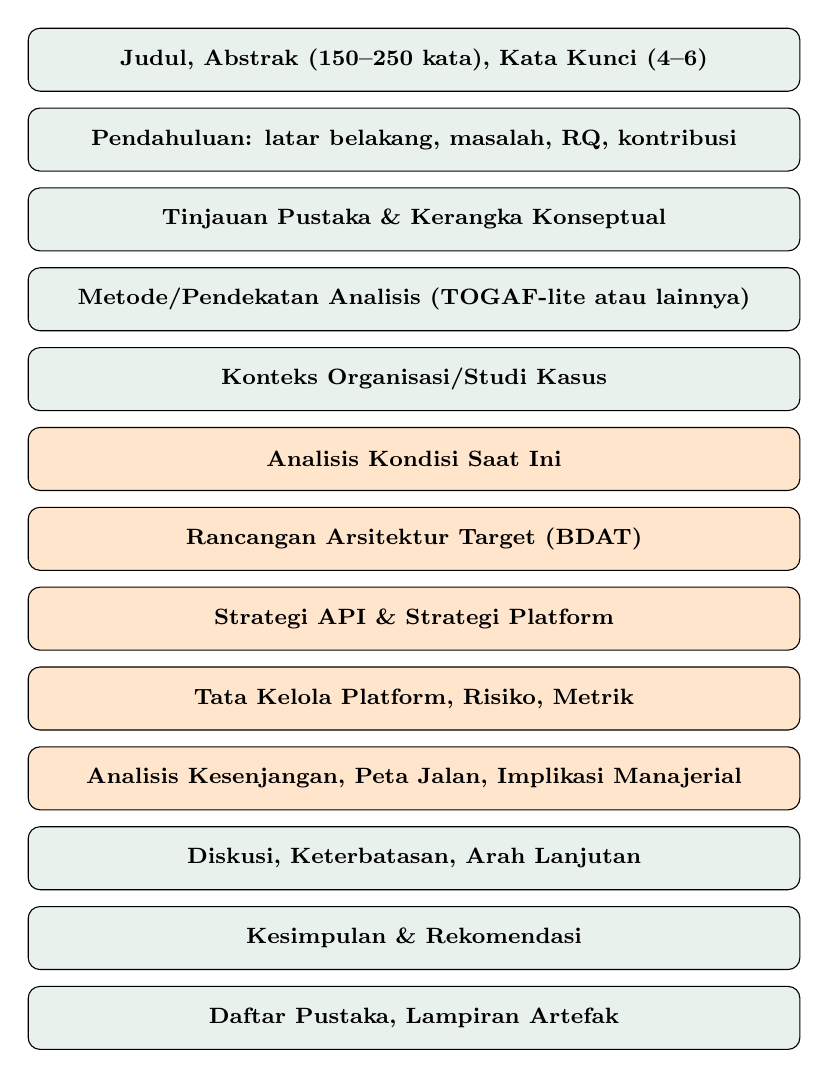
\begin{tikzpicture}[
  font=\footnotesize\bfseries,
  node distance=2mm,
  sec/.style={
    draw, rounded corners=1.5mm, align=left,
    minimum width=98mm, minimum height=8mm,
    fill=praditagreen!10,
    inner xsep=3mm
  },
  highlight/.style={sec, fill=orange!20}
]
\node[sec] (a) {Judul, Abstrak (150--250 kata), Kata Kunci (4--6)};
\node[sec, below=of a] (b) {Pendahuluan: latar belakang, masalah, RQ, kontribusi};
\node[sec, below=of b] (c) {Tinjauan Pustaka \& Kerangka Konseptual};
\node[sec, below=of c] (d) {Metode/Pendekatan Analisis (TOGAF-lite atau lainnya)};
\node[sec, below=of d] (e) {Konteks Organisasi/Studi Kasus};
\node[highlight, below=of e] (f) {Analisis Kondisi Saat Ini};
\node[highlight, below=of f] (g) {Rancangan Arsitektur Target (BDAT)};
\node[highlight, below=of g] (h) {Strategi API \& Strategi Platform};
\node[highlight, below=of h] (i) {Tata Kelola Platform, Risiko, Metrik};
\node[highlight, below=of i] (j) {Analisis Kesenjangan, Peta Jalan, Implikasi Manajerial};
\node[sec, below=of j] (k) {Diskusi, Keterbatasan, Arah Lanjutan};
\node[sec, below=of k] (l) {Kesimpulan \& Rekomendasi};
\node[sec, below=of l] (m) {Daftar Pustaka, Lampiran Artefak};
\end{tikzpicture}
}
\caption{Anatomi makalah publikasi yang akan dibangun sesi demi sesi. Bagian
berlatar oranye merupakan bagian teknis-substantif yang menjadi inti
kontribusi dan paling banyak dibangun pada Sesi~6 sampai Sesi~12.}
\label{fig:anatomi-makalah}
\end{figure}

Setiap bagian makalah memiliki tujuan komunikasi tersendiri.
\emph{Pendahuluan} meyakinkan pembaca bahwa masalah penting dan layak
dipelajari. \emph{Tinjauan pustaka} menempatkan makalah dalam percakapan
akademik yang sudah ada. \emph{Metode} menjelaskan bagaimana analisis
dilakukan agar dapat dievaluasi atau direplikasi. \emph{Analisis dan
rancangan} menyajikan kontribusi inti. \emph{Diskusi} mengubah temuan menjadi
makna dan implikasi. \emph{Kesimpulan} menutup argumen dengan jelas dan
menunjukkan arah lanjutan.

\section{Konteks Indonesia: Mengapa Lokal Itu Penting}

Banyak buku Enterprise Architecture ditulis dengan asumsi pasar, regulasi, dan
budaya organisasi Amerika Utara atau Eropa. Kondisi tersebut tidak selalu
sejalan dengan Indonesia. Karena itu, mata kuliah ini menempatkan konteks
Indonesia sebagai bagian inti analisis, bukan sekadar catatan tambahan.

Beberapa regulasi dan standar yang akan sering muncul dalam buku ini antara
lain:

\begin{itemize}
  \item \textbf{UU No.~27/2022 tentang Pelindungan Data Pribadi (UU PDP)}
        membentuk batas etis dan hukum tentang bagaimana data pelanggan boleh
        dikumpulkan, diproses, dan dipertukarkan.
  \item \textbf{UU No.~11/2008 jo.~UU No.~19/2016 tentang Informasi dan
        Transaksi Elektronik (UU ITE)} mengatur tanggung jawab penyelenggara
        sistem elektronik.
  \item \textbf{PP No.~71/2019 tentang Penyelenggaraan Sistem dan Transaksi
        Elektronik} mengatur penyelenggaraan sistem elektronik, termasuk
        aspek kedaulatan data dan klasifikasi
        sistem strategis.
  \item \textbf{Permenkominfo PSE} mewajibkan pendaftaran penyelenggara sistem
        elektronik baik publik maupun privat.
  \item \textbf{Standar Nasional Open API Pembayaran (SNAP BI)} dari Bank
        Indonesia membakukan integrasi API pada layanan pembayaran.
  \item \textbf{Ketentuan Otoritas Jasa Keuangan (OJK)} dan \textbf{Badan Siber
        dan Sandi Negara (BSSN)} memberi rambu untuk sektor keuangan dan
        keamanan siber nasional.
\end{itemize}

Selain regulasi, mahasiswa juga akan belajar dari ekosistem digital Indonesia:
Gojek, Tokopedia, Dana, Halodoc, Ruangguru, BCA Open API, BRI BRIAPI, Telkom
Indonesia, Kementerian PANRB melalui program Satu Data Indonesia, serta
koperasi/BPR dan BUMN di sektor energi, transportasi, dan telekomunikasi.
Studi kasus lokal diperkenalkan secara bertahap agar pembahasan tidak berhenti
pada abstraksi.

Tantangan implementasi yang khas Indonesia juga akan dibahas secara terbuka:
keterbatasan anggaran TI di banyak organisasi publik, kapasitas SDM yang
beragam, kematangan vendor lokal yang tidak merata, infrastruktur digital
yang berbeda antarwilayah, regulasi sektoral yang berlapis, serta budaya
organisasi yang sering kali masih hierarkis.

\section{Studi Kasus Mini: Memilih Posisi Bank Wanua}

Mari kita lanjutkan skenario Bank Wanua. Setelah dewan direksi sepakat untuk
melakukan transformasi digital, sebuah lokakarya satu hari diadakan untuk
menjawab tiga pertanyaan strategis berikut:

\begin{enumerate}
  \item Apakah Bank Wanua akan menjadi platform mandiri yang mengundang mitra
        UMKM dan fintech untuk masuk, atau akan bergabung sebagai mitra ke
        platform yang lebih besar (misalnya melalui SNAP BI dan kemitraan
        dengan dompet digital nasional)?
  \item Layanan apa yang sebaiknya dibuka sebagai \emph{public API} terlebih
        dahulu agar memberi nilai segera bagi UMKM, tanpa membahayakan keamanan
        dan kepatuhan?
  \item Kapabilitas internal apa yang harus diperkuat sebelum API publik
        tersebut layak diluncurkan?
\end{enumerate}

Lokakarya seperti ini, bila hanya diisi diskusi bebas, sering berakhir dengan
opini yang saling bertabrakan tanpa keputusan yang jelas. Enterprise
Architecture menyediakan kerangka analisis untuk memetakan kapabilitas, value
stream, kondisi saat ini, target, kesenjangan, dan peta jalan. Dengan begitu,
diskusi dapat bergerak dari adu pendapat menjadi argumen berbasis bukti.

Buku ini mengikuti keputusan tersebut secara konkret. Dari portofolio
kapabilitas yang disepakati Bank Wanua, \textbf{API Transfer dan Perpindahan
Dana}---``rel'' perpindahan uang yang membungkus BI-FAST---dipilih sebagai
kapabilitas sasaran yang dibedah lapis demi lapis sepanjang Bab~3 sampai Bab~5
(lihat Bagian~\ref{sec:studi-kasus-berjalan} di Pendahuluan). Pembaca menerapkan
pola analisis yang sama pada organisasi pilihannya sendiri.

Pada akhir Bab~13, Bank Wanua (atau organisasi pilihan pembaca) akan memiliki
peta kapabilitas bisnis dengan prioritas yang jelas, peta data beserta
kepemilikan dan klasifikasi sensitivitasnya, portofolio aplikasi dengan
rekomendasi tindak lanjut, rancangan arsitektur teknologi target, portofolio
API yang diprioritaskan berdasarkan dampak dan kelayakan, model platform
dengan analisis \emph{network effect}, piagam tata kelola platform yang
mempertimbangkan regulasi Indonesia, analisis kesenjangan, serta peta jalan
12--24 bulan. Semua artefak itu kemudian dirangkai menjadi satu makalah
publikasi.

\section{Memilih Target Publikasi}

Salah satu keputusan paling penting di Sesi~1 adalah memilih dua atau tiga
target publikasi. Target ini akan menentukan templat, panjang naskah, gaya
sitasi, dan cara argumen disusun. Target yang dipilih sebaiknya realistis
terhadap data dan akses yang dimiliki, sekaligus relevan dengan tema makalah.

\subsection{Jenis Target Publikasi dan Karakteristiknya}

Gambar~\ref{fig:venue-map} merangkum jenis target publikasi yang umum diakses oleh
mahasiswa pascasarjana di Indonesia.

\begin{figure}[htbp]
\centering
\resizebox{0.72\textwidth}{!}{
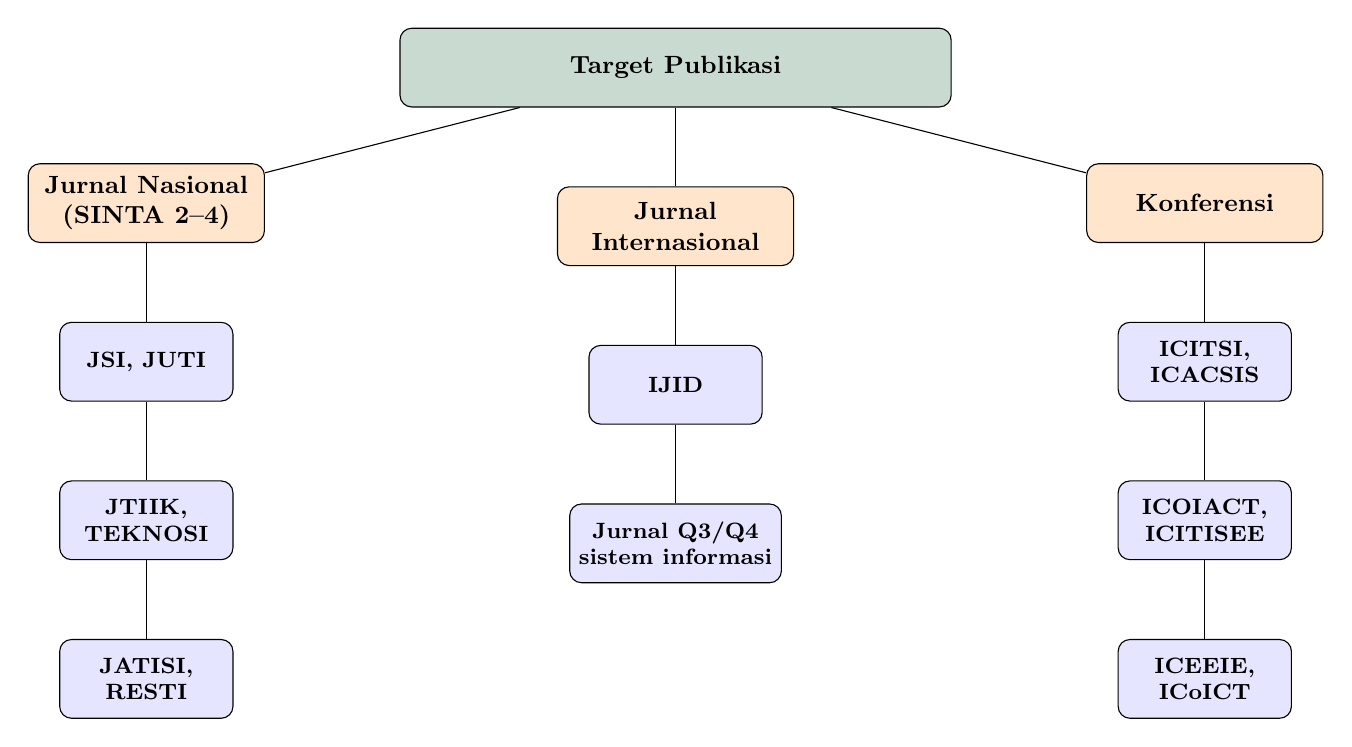
\begin{tikzpicture}[
  font=\small\bfseries,
  level distance=14mm,
  sibling distance=22mm,
  node distance=10mm,
  block/.style={
    draw, rounded corners=1.5mm, align=center,
    minimum width=30mm, minimum height=10mm
  },
  root/.style={block, fill=praditagreen!25, minimum width=70mm},
  cat/.style={block, fill=orange!20},
  ven/.style={block, fill=blue!10, minimum width=22mm, font=\footnotesize\bfseries}
]
\node[root] (root) {Target Publikasi};
\node[cat, below left=of root, xshift=-10mm] (jur) {Jurnal Nasional\\(SINTA 2--4)};
\node[cat, below=of root] (jurint) {Jurnal\\Internasional};
\node[cat, below right=of root, xshift=10mm] (kon) {Konferensi};

\node[ven, below=of jur] (j1) {JSI, JUTI};
\node[ven, below=of j1] (j2) {JTIIK,\\TEKNOSI};
\node[ven, below=of j2] (j3) {JATISI,\\RESTI};

\node[ven, below=of jurint] (i1) {IJID};
\node[ven, below=of i1] (i2) {Jurnal Q3/Q4\\sistem informasi};

\node[ven, below=of kon] (k1) {ICITSI,\\ICACSIS};
\node[ven, below=of k1] (k2) {ICOIACT,\\ICITISEE};
\node[ven, below=of k2] (k3) {ICEEIE,\\ICoICT};

\draw (root) -- (jur);
\draw (root) -- (jurint);
\draw (root) -- (kon);
\draw (jur) -- (j1);
\draw (j1) -- (j2);
\draw (j2) -- (j3);
\draw (jurint) -- (i1);
\draw (i1) -- (i2);
\draw (kon) -- (k1);
\draw (k1) -- (k2);
\draw (k2) -- (k3);
\end{tikzpicture}
}
\caption{Tiga jenis target publikasi yang umum diakses oleh mahasiswa pascasarjana
Indonesia. Daftar tidak eksklusif; status akreditasi/indeks wajib diverifikasi
saat semester berjalan.}
\label{fig:venue-map}
\end{figure}

\textbf{Jurnal nasional terakreditasi (SINTA 2--4)} cocok untuk makalah dengan
kontribusi yang jelas dan analisis mendalam pada studi kasus Indonesia. Proses
telaah biasanya berlangsung beberapa bulan; tidak selalu ada tenggat kaku,
tetapi mahasiswa tetap perlu memperhatikan ritme penerbitan jurnal.

\textbf{Jurnal internasional (Q3--Q4)} cocok jika mahasiswa ingin pengalaman
proses telaah yang lebih ketat dan jangkauan pembaca yang lebih luas. Proses
telaah dapat berlangsung lebih lama, dan biaya publikasi pada sebagian jurnal
cukup besar. Reputasi jurnal harus selalu diperiksa agar mahasiswa terhindar
dari jurnal yang dicurigai \emph{predatory}.

\textbf{Konferensi nasional/internasional} cocok untuk mahasiswa yang ingin
menyelesaikan makalah dengan tenggat yang lebih jelas. Konferensi seperti
ICITSI, ICACSIS, ICOIACT, ICITISEE, ICEEIE, dan ICoICT dapat menjadi pintu
masuk pertama mahasiswa pascasarjana ke komunitas akademik yang lebih luas.
Status indeks, penerbit, jadwal, dan jalur/topik konferensi tetap harus
diverifikasi pada semester berjalan.

\subsection{Kriteria Pemilihan Target Publikasi}

Lima kriteria praktis berikut dapat membantu mahasiswa memilih target
publikasi:

\begin{enumerate}
  \item \textbf{Kesesuaian ruang lingkup:} apakah topik makalah cocok dengan
        ruang lingkup atau jalur/topik target publikasi?
  \item \textbf{Kelayakan akses data:} apakah data dan akses organisasi yang
        dimiliki cukup untuk memenuhi kedalaman analisis yang diharapkan?
  \item \textbf{Reputasi dan keberlanjutan:} apakah target publikasi memiliki
        reputasi yang jelas, terindeks dengan benar, dan terbit secara
        konsisten?
  \item \textbf{Tenggat dan kalender:} apakah tenggat pengajuan cocok dengan
        kalender akademik mata kuliah?
  \item \textbf{Biaya:} berapa biaya \emph{article processing charge} (APC)
        atau \emph{registration fee}? Apakah terjangkau atau tersedia subsidi?
\end{enumerate}

Pada Sesi~1, mahasiswa diharapkan memilih dua atau tiga target publikasi dan
melakukan verifikasi singkat terhadap kelima kriteria di atas. Verifikasi ini
bukan sekadar formalitas; ia akan memengaruhi struktur makalah yang ditulis
sepanjang semester.

\section{Tipe Makalah yang Dapat Dipilih}

Makalah yang dihasilkan dari mata kuliah ini dapat mengambil salah satu dari
empat bentuk berikut, sesuai minat mahasiswa dan akses data yang tersedia:

\begin{enumerate}
  \item \textbf{Studi kasus arsitektur enterprise:} analisis kondisi saat
        ini, rancangan target, dan peta jalan transformasi pada satu
        organisasi. Cocok jika mahasiswa
        memiliki akses cukup pada dokumen, proses, atau narasumber organisasi.
  \item \textbf{Design science atau rancangan solusi:} perancangan blueprint,
        strategi API, atau model tata kelola sebagai artefak solusi. Cocok jika
        masalah organisasi cukup jelas dan mahasiswa ingin menonjolkan
        kontribusi rancangan.
  \item \textbf{Evaluasi strategi platform/API:} analisis ekonomi API,
        ekosistem platform, network effects, dan tata kelola pada satu kasus.
        Cocok jika studi kasus memiliki aspek ekosistem, mitra, atau open API.
  \item \textbf{Kajian konseptual berbasis kasus lokal:} sintesis literatur dan
        contoh Indonesia untuk menghasilkan kerangka atau rekomendasi. Cocok
        jika akses data organisasi terbatas namun literatur dan data sekunder
        tersedia.
\end{enumerate}

Tipe makalah dipilih bersamaan dengan target publikasi di Sesi~1, lalu
diperhalus kembali pada Sesi~2--3 setelah rumusan masalah dan akses data lebih
jelas.

\section{Glosarium Mini}

Beberapa istilah kunci yang akan sering muncul:

\begin{itemize}
  \item \textbf{Enterprise Architecture (EA):} disiplin yang menyelaraskan
        strategi organisasi dengan kapabilitas teknologi melalui pemetaan,
        prinsip, dan keputusan terdokumentasi.
  \item \textbf{TOGAF-lite:} versi sederhana dari The Open Group Architecture
        Framework yang berfokus pada siklus inti: visi, kondisi saat ini,
        target, kesenjangan, dan peta jalan, tanpa membawa seluruh
        kompleksitas TOGAF.
  \item \textbf{BDAT:} singkatan dari Business, Data, Application, Technology
        sebagai empat domain arsitektur klasik.
  \item \textbf{ArchiMate:} bahasa pemodelan standar untuk arsitektur
        enterprise; menyusun arsitektur ke dalam lapisan motivasi, strategi,
        bisnis, aplikasi, teknologi/fisik, serta implementasi dan migrasi.
  \item \textbf{API (Application Programming Interface):} kontrak digital
        terstandar yang memungkinkan satu sistem berinteraksi dengan sistem
        lain.
  \item \textbf{Platform multi-sided:} model bisnis yang menghubungkan dua atau
        lebih kelompok pengguna dan menghasilkan \emph{network effect}.
  \item \textbf{Network effect:} fenomena bahwa nilai sebuah produk/platform
        meningkat bersamaan dengan bertambahnya pengguna pada satu atau lebih
        sisi platform.
  \item \textbf{Research question (RQ):} pertanyaan penelitian yang menjadi
        arah utama makalah dan dijawab melalui analisis serta pembahasan.
\end{itemize}

\section{Integrasi ke Makalah Publikasi}

Bab ini menyumbang bahan awal untuk dua bagian makalah:

\begin{itemize}
  \item \textbf{Pendahuluan:} pembaca akan menggunakan skenario organisasi
        sendiri (serupa dengan Bank Wanua) sebagai latar belakang makalah,
        kemudian
        menuliskan motivasi mengapa transformasi digital pada organisasi
        tersebut layak dianalisis.
  \item \textbf{Pernyataan kontribusi:} pernyataan singkat 2--3 kalimat
        tentang apa yang akan dihasilkan makalah dan mengapa hasil tersebut
        bernilai bagi komunitas akademik atau praktik.
\end{itemize}

Pada Sesi~2, RQ dan pernyataan kontribusi akan dipertajam. Pada Sesi~1, yang
dibutuhkan adalah draf awal yang cukup jelas untuk menjadi titik pijak.
Naskah belum perlu sempurna; yang penting cukup konkret untuk ditinjau bersama
dosen dan rekan sejawat.

\section{Diskusi Kritis dan Perangkap Umum}

Beberapa perangkap berikut sering muncul ketika mahasiswa pertama kali masuk
ke materi Enterprise Architecture:

\begin{enumerate}
  \item \emph{Memulai dari teknologi.} Mahasiswa sering tergoda memilih
        teknologi terlebih dahulu, misalnya ``saya ingin menulis tentang
        microservices'', alih-alih memulai dari masalah organisasi.
  \item \emph{Topik terlalu luas.} ``Transformasi digital BUMN energi
        nasional'' adalah judul tesis lima tahun, bukan makalah satu semester.
        Pilih satu organisasi, satu fokus.
  \item \emph{Mengabaikan konteks Indonesia.} Mengutip teori platform Silicon
        Valley tanpa menyelaraskan dengan UU PDP, OJK, atau realitas pasar
        lokal akan menghasilkan rekomendasi yang tidak dapat
        diimplementasikan.
  \item \emph{Memilih target publikasi setelah makalah selesai.} Akibatnya
        format, panjang, dan referensi tidak selaras dengan templat. Pilih
        target publikasi di Sesi~1 dan ikuti templat tersebut sejak awal.
  \item \emph{Menganggap blueprint sebagai luaran utama.} Blueprint adalah
        bukti analisis; luaran utama tetap makalah.
\end{enumerate}

\section{Latihan Terapan Individual}

Latihan pada bab ini sengaja dibuat ringan karena fungsinya adalah meletakkan
fondasi yang akan ditindaklanjuti pada bab-bab selanjutnya.

\subsection*{Latihan~2.1: Pemilihan Organisasi Studi Kasus (45 menit)}

Pilihlah satu organisasi nyata atau hipotetis-realistis dalam konteks
Indonesia yang akan Anda gunakan sebagai studi kasus sepanjang semester.
Tuliskan jawaban atas pertanyaan berikut secara ringkas (maksimum satu
halaman):

\begin{enumerate}
  \item Nama organisasi (boleh anonim/disamarkan, misalnya ``Bank Wanua'').
  \item Sektor (publik, pendidikan, kesehatan, keuangan, retail, logistik,
        manufaktur, sosial, layanan digital).
  \item Skala dan jangkauan operasi singkat.
  \item Mengapa organisasi ini menarik untuk dianalisis (1--2 paragraf).
  \item Akses data yang Anda miliki: dokumen publik, wawancara, observasi,
        data internal dengan izin, atau kombinasi.
\end{enumerate}

\subsection*{Latihan~2.2: Pernyataan Topik Awal (30 menit)}

Tuliskan satu paragraf (4--6 kalimat) sebagai pernyataan topik awal makalah
Anda. Paragraf ini sebaiknya menjawab tiga hal:

\begin{itemize}
  \item Apa masalah/peluang transformasi digital yang akan dianalisis?
  \item Pendekatan analisis apa yang akan digunakan (TOGAF-lite, design
        science, evaluasi platform, atau kajian konseptual)?
  \item Apa potensi kontribusi makalah bagi komunitas akademik atau praktik?
\end{itemize}

\subsection*{Latihan~2.3: Identifikasi 2--3 Target Publikasi (60 menit)}

Pilih dua atau tiga target publikasi (jurnal SINTA, jurnal internasional, atau
konferensi) yang relevan dengan topik Anda. Buat tabel ringkas dengan kolom:
nama target publikasi, ruang lingkup atau jalur/topik yang relevan, status
indeks atau akreditasi, biaya publikasi/APC, tenggat atau jadwal terbit, dan
tautan templat.

\subsection*{Latihan~2.4: Telaah Singkat Satu Makalah Contoh (60 menit)}

Cari satu makalah akademik (jurnal SINTA, jurnal internasional, atau prosiding
konferensi) yang relevan dengan topik Anda. Tuliskan refleksi satu halaman:

\begin{itemize}
  \item Apa pertanyaan penelitian (research question) makalah tersebut?
  \item Pendekatan/metode apa yang digunakan?
  \item Apa kontribusinya?
  \item Bagaimana makalah itu menempatkan konteks (Indonesia atau lainnya)?
  \item Apa yang dapat Anda pelajari dari makalah itu untuk naskah Anda?
\end{itemize}

\subsection*{Pertanyaan Refleksi}

\begin{enumerate}
  \item Apakah organisasi yang Anda pilih cukup spesifik untuk dianalisis
        dalam satu semester?
  \item Apakah akses data yang Anda miliki memungkinkan tipe makalah yang
        Anda pilih?
  \item Target publikasi mana yang paling realistis dilihat dari tenggat,
        biaya, dan kedalaman analisis yang dapat Anda capai?
  \item Setelah menelaah satu makalah contoh, bagian mana yang menurut Anda
        akan paling menantang ditulis?
\end{enumerate}

\section{Uji Mandiri}

\subsection*{Pertanyaan Konseptual}

\begin{enumerate}
  \item Jelaskan dengan kata-kata Anda sendiri mengapa Enterprise Architecture
        penting bagi pengambil keputusan non-IT.
  \item Sebutkan empat domain BDAT dan beri satu contoh artefak per domain.
  \item Apa yang dimaksud dengan \emph{network effect} pada platform
        multi-sided? Beri satu contoh dari Indonesia.
  \item Sebutkan minimal lima bagian pada anatomi makalah ilmiah dan jelaskan
        fungsi komunikasi setiap bagian.
  \item Apa perbedaan utama antara API \emph{private}, \emph{partner}, dan
        \emph{public}?
\end{enumerate}

\subsection*{Pertanyaan Aplikatif}

\begin{enumerate}
  \item Sebuah rumah sakit daerah ingin membangun layanan telekonsultasi.
        Sebutkan tiga keputusan EA strategis (lintas BDAT) yang perlu
        dipertimbangkan oleh direksi rumah sakit.
  \item Sebuah koperasi simpan-pinjam ingin membuka API agar UMKM dapat
        mengintegrasikan layanan pembayarannya. Apa risiko utama dari sisi
        regulasi dan tata kelola yang perlu diantisipasi?
\end{enumerate}

\subsection*{Pertanyaan Reflektif untuk Makalah}

\begin{enumerate}
  \item Bagian mana dari latihan~2.1--2.4 yang paling akan memengaruhi
        struktur Pendahuluan makalah Anda?
  \item Apakah ada kemungkinan organisasi studi kasus Anda berubah dalam dua
        bab pertama? Apa indikatornya?
\end{enumerate}

\section{Ringkasan Bab}

Bab ini memperkenalkan empat pilar yang menjadi dasar seluruh mata kuliah.
Pertama, Enterprise Architecture diposisikan sebagai jembatan dua arah antara
strategi organisasi dan kapabilitas teknologi. Kedua, kerangka BDAT (Business,
Data, Application, Technology) diperkenalkan sebagai cara memecah kerumitan
organisasi menjadi empat domain yang saling terkait. Ketiga, API dan platform
diposisikan sebagai pengungkit nilai pada model bisnis digital modern, dengan
studi kasus Indonesia sebagai sumber pembelajaran utama. Keempat, anatomi
makalah ilmiah diperkenalkan sebagai kerangka komunikasi yang akan dibangun
sesi demi sesi.

Konteks Indonesia dipertegas sebagai bagian inti analisis melalui regulasi
seperti UU PDP, UU ITE, PP 71/2019, Permenkominfo PSE, OJK, BSSN, dan SNAP
BI, serta melalui ekosistem digital yang akan sering digunakan sebagai studi
kasus. Pemilihan target publikasi juga diperkenalkan sebagai keputusan
strategis yang memengaruhi struktur makalah. Lima kriteria praktisnya adalah
kesesuaian ruang lingkup, kelayakan akses data, reputasi target publikasi,
tenggat, dan biaya.

Pada akhir bab, mahasiswa telah memilih satu organisasi studi kasus, menulis
pernyataan topik awal, dan mengidentifikasi dua sampai tiga kandidat target
publikasi. Tiga keluaran awal ini menjadi titik pijak Bab~3, ketika rumusan
masalah, pertanyaan penelitian, dan pernyataan kontribusi dipertajam melalui
\emph{lapisan motivasi} ArchiMate---pemangku kepentingan, pendorong, sasaran,
kebutuhan, dan kendala---pada studi kasus API Transfer Dana.

\section{Jembatan ke Bab Berikutnya}

Bab~3 masuk ke \emph{lapisan motivasi}---lapisan teratas dalam bahasa pemodelan
ArchiMate yang merekam \emph{mengapa} sebuah arsitektur dibangun. Untuk studi
kasus berjalan, yaitu API Transfer dan Perpindahan Dana Bank Wanua
(Bagian~\ref{sec:studi-kasus-berjalan}), pembaca memetakan pemangku kepentingan
beserta kekhawatirannya, pendorong perubahan, asesmen kondisi saat ini, sasaran,
hasil, kebutuhan, kendala, dan prinsip. Dari peta motivasi itu, ketidakselarasan
antara sasaran dan kapabilitas yang tersedia diubah menjadi rumusan masalah,
pertanyaan penelitian, dan pernyataan kontribusi makalah secara lebih tajam.

\section{Bacaan Lanjutan}

\subsection*{Bacaan Inti}

\begin{itemize}
  \item \emph{TOGAF Standard, 10th Edition}~\cite{togaf10}. Bagian pengantar
        (\emph{Architecture Development Method overview}) memberi gambaran
        besar sebelum pembaca masuk ke versi ``lite'' pada Bab~4.
  \item \emph{Designed for Digital}~\cite{ross2019designed}. Cocok untuk
        membangun intuisi tentang mengapa transformasi digital membutuhkan kerangka
        arsitektur.
  \item \emph{Platform Revolution}~\cite{parker2016platform}. Bab pertama
        mengenai pergeseran dari model linear ke platform sangat membantu
        untuk memahami kasus seperti Gojek dan Tokopedia.
\end{itemize}

\subsection*{Bacaan untuk Memperdalam}

\begin{itemize}
  \item \emph{APIs: A Strategy Guide}~\cite{jacobson2011apis}. Untuk pembaca
        yang ingin memperluas wawasan API sebelum Bab~10.
  \item \emph{The Business of Platforms}~\cite{cusumano2019business}.
        Bacaan pelengkap untuk memahami strategi dan tata kelola platform.
  \item \emph{Enterprise Architecture as Strategy}~\cite{ross2006enterprise}.
        Rujukan klasik EA yang relevan untuk argumen keselarasan bisnis--TI.
\end{itemize}

\subsection*{Sumber Indonesia}

\begin{itemize}
  \item \emph{Standar Nasional Open API Pembayaran (SNAP BI)}~\cite{snapbi}.
        Dokumen resmi bagi mahasiswa yang memilih topik perbankan/fintech.
  \item \emph{Satu Data Indonesia}~\cite{satudata}. Kerangka tata kelola data
        publik nasional yang relevan untuk studi kasus pemerintahan.
  \item \emph{Undang-Undang Pelindungan Data Pribadi}~\cite{uupdp2022} dan
        \emph{PP No.~71/2019}~\cite{pp712019} menjadi dua rujukan regulasi
        yang akan sering muncul sepanjang buku.
  \item Jurnal Sistem Informasi (JSI), JUTI, JTIIK, TEKNOSI, dan jurnal SINTA
        lain dengan ruang lingkup EA, sistem informasi, atau platform; gunakan SINTA
        \footnote{\url{https://sinta.kemdiktisaintek.go.id/}} dan Garuda
        \footnote{\url{https://garuda.kemdiktisaintek.go.id/}} untuk mencari
        makalah relevan.
\end{itemize}

    \chapter[Strategi Bisnis dan Rumusan Masalah]{Strategi Bisnis dan Rumusan
Masalah: Menyelaraskan Arah Organisasi dengan Pertanyaan Penelitian}
\label{ch:strategi-bisnis}



\section*{Tujuan Pembelajaran}
\begin{itemize}
  \item Menjelaskan hubungan antara strategi organisasi, model bisnis,
        kapabilitas utama, dan kebutuhan arsitektur enterprise dengan bahasa
        manajerial.
  \item Menggunakan kanvas model bisnis dan konsep \emph{operating model}
        untuk membaca arah strategis organisasi studi kasus.
  \item Mengidentifikasi ketidakselarasan antara strategi bisnis dan keputusan
        teknologi sebagai sumber masalah penelitian.
  \item Merumuskan rumusan masalah, pertanyaan penelitian (RQ), dan kontribusi
        awal yang layak dikembangkan menjadi makalah publikasi individual.
\end{itemize}


\section{Ringkasan Awal Bab}

Bab ini membahas cara mengubah topik awal menjadi rumusan masalah, pertanyaan
penelitian, dan kontribusi makalah. Pembahasan dimulai dari dilema organisasi:
strategi digital sering terdengar jelas di tingkat slogan, tetapi tidak selalu
selaras dengan proses, data, aplikasi, teknologi, API, dan tata kelola yang
dimiliki organisasi. Untuk membaca ketegangan tersebut, bab ini menggunakan
kanvas model bisnis dan konsep \emph{operating model} sebagai alat analisis
yang ramah bagi pembaca non-IT. Melalui studi kasus Bank Wanua, pembaca
melihat bagaimana strategi menjadi mitra digital UMKM dapat diterjemahkan
menjadi daftar ketidakselarasan, lalu diubah menjadi rumusan masalah, RQ, dan
pernyataan kontribusi. Keluaran bab ini memperkuat bagian Pendahuluan makalah,
terutama latar belakang masalah, RQ, dan kontribusi awal.

\section{Pendahuluan}

Bab sebelumnya membantu pembaca memilih organisasi studi kasus, menulis
pernyataan topik awal, dan mengenali target publikasi yang realistis. Bab ini
melangkah satu tahap lebih jauh: topik awal tersebut harus diubah menjadi
masalah penelitian yang tajam. Dalam makalah publikasi, masalah yang tajam
lebih penting daripada topik yang terdengar menarik. Topik menyebut area
umum, sedangkan masalah menjelaskan ketegangan yang layak dianalisis, bukti
yang perlu dikumpulkan, dan kontribusi yang dapat diberikan.

Bagi pembaca non-IT, strategi bisnis menjadi titik mulai yang sehat. Banyak
inisiatif digital gagal bukan karena teknologi yang dipilih terlalu lemah,
melainkan karena arah bisnis, model operasi, dan prioritas teknologi tidak
dibaca sebagai satu kesatuan. Organisasi ingin bergerak cepat, tetapi datanya
tersebar. Organisasi ingin membuka layanan digital, tetapi proses internal
masih manual. Organisasi ingin membangun platform, tetapi belum jelas siapa
pengguna utama dan nilai apa yang dipertukarkan. Dalam bahasa Enterprise
Architecture, persoalan seperti ini adalah persoalan keselarasan antara
strategi dan kapabilitas.

Rujukan klasik Enterprise Architecture menempatkan arsitektur sebagai fondasi
pelaksanaan strategi bisnis, bukan sekadar urusan diagram teknologi
\cite{ross2006enterprise}. Pandangan yang lebih baru juga menekankan bahwa
organisasi digital membutuhkan kapabilitas yang dirancang secara sadar agar
strategi dapat dieksekusi berulang, aman, dan terukur \cite{ross2019designed}.
Karena itu, Bab 2 mengajak pembaca membaca strategi organisasi dengan dua alat
sederhana: kanvas model bisnis dan konsep \emph{operating model}. Keduanya
dipakai untuk menyusun rumusan masalah, RQ, dan pernyataan kontribusi awal.

\section{Skenario Pembuka: Ketika Strategi Digital Tidak Menyatu}

Bank Wanua, yang diperkenalkan pada Bab~\ref{ch:orientasi}, kini sudah
menetapkan ambisi strategis baru. Dalam tiga tahun, bank daerah ini ingin
menjadi mitra keuangan digital utama bagi UMKM lokal. Direksi membayangkan
aplikasi mobile yang lebih baik, layanan pembayaran yang terhubung dengan
ekosistem QRIS, API untuk mitra koperasi dan marketplace lokal, serta program
analitik sederhana untuk membaca kebutuhan nasabah UMKM.

Namun setelah beberapa bulan berjalan, tanda-tanda ketidakselarasan mulai
muncul. Tim pemasaran menjanjikan pembukaan rekening digital yang cepat, tetapi
tim operasional masih membutuhkan verifikasi manual berlapis. Tim TI diminta
membangun API untuk mitra, tetapi daftar layanan prioritas belum disepakati.
Divisi kepatuhan meminta kontrol data yang ketat, sementara unit bisnis ingin
kampanye yang lebih personal. Kantor cabang ingin mempertahankan relasi tatap
muka dengan nasabah, tetapi kantor pusat menekan efisiensi melalui kanal
digital.

Masalah Bank Wanua bukan sekadar ``belum punya aplikasi yang bagus''. Masalah
yang lebih mendasar adalah belum jelasnya hubungan antara strategi, model
bisnis, model operasi, dan keputusan arsitektur. Jika mahasiswa langsung
menulis makalah tentang ``perancangan aplikasi mobile Bank Wanua'', naskahnya
mungkin terlalu sempit. Jika mahasiswa menulis tentang ``transformasi digital
Bank Wanua'', naskahnya mungkin terlalu luas. Tantangannya adalah menemukan
rumusan masalah yang berada di tengah: cukup sempit untuk dianalisis dalam
satu semester, tetapi cukup strategis untuk memberi kontribusi akademik dan
praktis.

\subsection*{Pertanyaan Pemandu Bab Ini}

\begin{enumerate}
  \item Strategi bisnis apa yang sebenarnya sedang dikejar organisasi studi
        kasus?
  \item Bagaimana model bisnis organisasi menghasilkan nilai bagi pelanggan,
        mitra, dan pemangku kepentingan lain?
  \item Model operasi seperti apa yang dibutuhkan agar strategi tersebut dapat
        dijalankan secara konsisten?
  \item Di mana letak ketidakselarasan antara strategi, proses, data, aplikasi,
        teknologi, API, dan tata kelola?
  \item Bagaimana ketidakselarasan itu diubah menjadi rumusan masalah, RQ, dan
        kontribusi awal makalah?
\end{enumerate}

\section{Mengapa Topik Ini Penting bagi Pembaca Non-IT}

Pembaca non-IT tidak harus menjadi arsitek teknis untuk dapat membaca masalah
strategi digital. Yang dibutuhkan adalah kemampuan melihat pola: apa tujuan
organisasi, siapa pengguna yang dilayani, nilai apa yang dijanjikan, proses apa
yang harus berubah, data apa yang dibutuhkan, dan keputusan apa yang berisiko
jika tidak dikelola. Kemampuan ini sering justru berada dekat dengan peran
manajerial, karena manajer melihat dampak keputusan teknologi pada pelanggan,
pegawai, anggaran, regulasi, dan reputasi.

Dalam organisasi nyata, pertanyaan teknis hampir selalu membawa konsekuensi
manajerial. Membuka API bukan hanya pekerjaan membuat endpoint; ia mengubah
cara organisasi berhubungan dengan mitra. Memusatkan data pelanggan bukan
hanya pekerjaan integrasi; ia memunculkan pertanyaan tentang kepemilikan data,
izin pemrosesan, dan perlindungan privasi. Mengganti aplikasi lama bukan hanya
pekerjaan pengadaan; ia mengganggu kebiasaan kerja, proses persetujuan, dan
indikator kinerja.

Karena itu, rumusan masalah dalam makalah Enterprise Architecture tidak cukup
berbunyi ``sistem belum terintegrasi''. Rumusan yang lebih kuat menjelaskan
mengapa integrasi itu penting bagi strategi, siapa yang terkena dampaknya, apa
bukti ketidakselarasannya, dan bagaimana analisis arsitektur dapat membantu
pengambil keputusan. Bab ini memberi kerangka untuk melakukan penyempitan
tersebut.

\section{Konsep Inti: Strategi, Model Bisnis, dan RQ}

Empat konsep inti digunakan dalam bab ini. Pertama, \textbf{strategi bisnis}
menjelaskan pilihan organisasi tentang posisi, pelanggan, nilai, dan prioritas.
Kedua, \textbf{model bisnis} menjelaskan bagaimana organisasi menciptakan,
menyampaikan, dan menangkap nilai. Ketiga, \textbf{operating model} menjelaskan
tingkat standardisasi proses dan integrasi data yang dibutuhkan agar strategi
dapat dijalankan \cite{ross2006enterprise}. Keempat, \textbf{rumusan masalah
dan RQ} menerjemahkan ketegangan strategis menjadi pertanyaan akademik yang
dapat dijawab melalui analisis.

\subsection{Strategi Bisnis: Pilihan, Bukan Slogan}

Strategi sering ditulis sebagai slogan: ``menjadi pemimpin digital'', ``memberi
layanan terbaik'', atau ``mendorong inovasi''. Slogan semacam itu tidak salah,
tetapi belum cukup untuk menjadi dasar arsitektur. Strategi yang dapat
diterjemahkan ke dalam arsitektur harus memperlihatkan pilihan. Pilihan itu
meliputi pelanggan mana yang diprioritaskan, layanan mana yang menjadi
pembeda, proses mana yang perlu distandardisasi, dan risiko mana yang bersedia
ditanggung.

Dalam konteks Bank Wanua, strategi ``menjadi mitra digital UMKM'' baru
bermakna jika diterjemahkan ke pertanyaan yang lebih konkret. Apakah bank
ingin memperluas basis nasabah baru, memperdalam hubungan dengan nasabah
lama, menjadi penyedia API untuk mitra, atau menjadi bagian dari ekosistem
platform yang lebih besar? Setiap pilihan membawa konsekuensi arsitektur yang
berbeda. Strategi akuisisi nasabah membutuhkan kanal digital dan verifikasi
identitas. Strategi kemitraan API membutuhkan kontrak layanan, keamanan, dan
tata kelola mitra. Strategi efisiensi cabang membutuhkan perubahan proses
operasi.

\subsection{Kanvas Model Bisnis: Membaca Cara Organisasi Menghasilkan Nilai}

Kanvas model bisnis membantu pembaca memetakan organisasi dalam sembilan
komponen yang mudah dibaca. Untuk kebutuhan bab ini, kanvas tidak dipakai
sebagai latihan kewirausahaan, melainkan sebagai alat untuk menghubungkan
strategi dengan kapabilitas arsitektur.

\begin{table}[htbp]
\centering
\scriptsize
\caption{Pertanyaan panduan kanvas model bisnis untuk analisis arsitektur.}
\label{tab:bmc-pertanyaan}
\begin{tabularx}{\textwidth}{@{}p{0.26\textwidth} X@{}}
\hline
\textbf{Komponen} & \textbf{Pertanyaan Arsitektural} \\
\hline
Segmen pelanggan & Kelompok pengguna mana yang paling penting, dan data apa
yang dibutuhkan untuk memahami kebutuhan mereka? \\
Proposisi nilai & Nilai apa yang dijanjikan, dan kapabilitas apa yang harus
ada agar janji itu dapat ditepati? \\
Kanal & Kanal fisik dan digital apa yang dipakai, dan bagaimana kanal tersebut
perlu terintegrasi? \\
Relasi pelanggan & Hubungan seperti apa yang dibangun: personal, otomatis,
komunitas, atau berbasis mitra? \\
Sumber pendapatan & Nilai ekonomi apa yang dihasilkan, dan metrik apa yang
dapat menunjukkan keberhasilannya? \\
Aktivitas kunci & Proses apa yang menentukan keberhasilan strategi? \\
Sumber daya kunci & Data, aplikasi, SDM, infrastruktur, dan mitra apa yang
menjadi sumber kemampuan utama? \\
Mitra kunci & Pihak luar mana yang perlu terhubung, dan aturan integrasi apa
yang dibutuhkan? \\
Struktur biaya & Biaya apa yang paling besar, dan keputusan arsitektur apa
yang dapat mengendalikannya? \\
\hline
\end{tabularx}
\end{table}

Kekuatan kanvas ini adalah kesederhanaannya. Pembaca dapat menggunakannya
untuk melihat apakah masalah digital yang dipilih benar-benar terhubung dengan
nilai organisasi. Jika sebuah inisiatif teknologi tidak jelas hubungannya
dengan pelanggan, proposisi nilai, aktivitas kunci, atau mitra, maka inisiatif
itu perlu dipertanyakan sebelum masuk ke rancangan arsitektur.

\subsection{Operating Model: Tingkat Integrasi dan Standardisasi}

\emph{Operating model} menjelaskan bagaimana organisasi menjalankan strategi
melalui proses dan data. Dalam rujukan Enterprise Architecture, dua pertanyaan
kunci digunakan untuk membaca model operasi: seberapa besar proses perlu
distandardisasi, dan seberapa besar data perlu diintegrasikan
\cite{ross2006enterprise}. Dari dua pertanyaan ini muncul empat pola umum.

\begin{figure}[htbp]
\centering
\scalebox{0.95}{
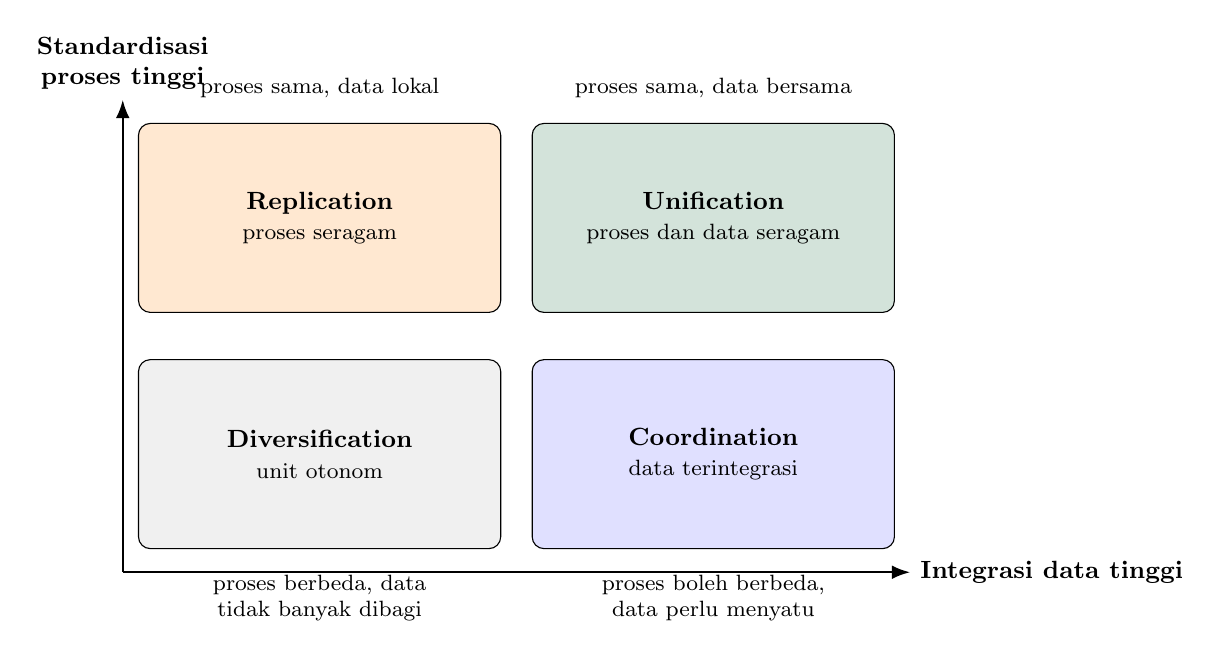
\begin{tikzpicture}[
  font=\small,
  axis/.style={-Latex, thick},
  cell/.style={draw, rounded corners=1.5mm, align=center,
    minimum width=46mm, minimum height=24mm},
  note/.style={font=\footnotesize\mdseries, align=center, text width=42mm}
]
  \draw[axis] (0,0) -- (10,0) node[right] {\textbf{Integrasi data tinggi}};
  \draw[axis] (0,0) -- (0,6) node[above, align=center] {\textbf{Standardisasi}\\\textbf{proses tinggi}};

  \node[cell, fill=gray!12] (div) at (2.5,1.5)
    {\textbf{Diversification}\\\footnotesize unit otonom};
  \node[cell, fill=blue!12] (coord) at (7.5,1.5)
    {\textbf{Coordination}\\\footnotesize data terintegrasi};
  \node[cell, fill=orange!18] (rep) at (2.5,4.5)
    {\textbf{Replication}\\\footnotesize proses seragam};
  \node[cell, fill=praditagreen!20] (uni) at (7.5,4.5)
    {\textbf{Unification}\\\footnotesize proses dan data seragam};

  \node[note, below=2mm of div] {proses berbeda, data tidak banyak dibagi};
  \node[note, below=2mm of coord] {proses boleh berbeda, data perlu menyatu};
  \node[note, above=2mm of rep] {proses sama, data lokal};
  \node[note, above=2mm of uni] {proses sama, data bersama};
\end{tikzpicture}
}
\caption{Empat pola operating model berdasarkan kebutuhan standardisasi proses
dan integrasi data.}
\label{fig:operating-model}
\end{figure}

Pola \emph{Diversification} cocok ketika unit bisnis relatif mandiri. Pola
\emph{Coordination} cocok ketika unit dapat bekerja berbeda, tetapi perlu
berbagi data pelanggan atau transaksi. Pola \emph{Replication} cocok ketika
organisasi ingin menyalin proses yang sama di banyak lokasi. Pola
\emph{Unification} cocok ketika proses dan data perlu sangat seragam, misalnya
untuk kepatuhan, layanan nasional, atau efisiensi besar-besaran.

Pemilihan operating model bukan sekadar label. Ia membantu mahasiswa
menjelaskan mengapa sebuah masalah arsitektur muncul. Jika strategi organisasi
membutuhkan koordinasi data pelanggan lintas unit, tetapi setiap unit
menyimpan data dengan definisi berbeda, maka ketidakselarasan itu dapat menjadi
sumber rumusan masalah. Jika organisasi menginginkan layanan digital yang sama
di seluruh cabang, tetapi proses cabang sangat berbeda, maka masalahnya bukan
hanya aplikasi, melainkan standardisasi proses.

\subsection{Rumusan Masalah, RQ, dan Kontribusi}

Rumusan masalah adalah pernyataan tentang ketegangan yang layak dianalisis.
Pertanyaan penelitian atau RQ adalah bentuk tanya yang membatasi arah
analisis. Kontribusi adalah janji tentang nilai yang akan diberikan makalah
kepada pembaca akademik atau praktisi.

Hubungan ketiganya dapat diringkas sebagai berikut:

\begin{itemize}
  \item \textbf{Rumusan masalah} menjawab: apa ketegangan utama yang terjadi?
  \item \textbf{RQ} menjawab: pertanyaan apa yang akan dijawab makalah?
  \item \textbf{Kontribusi} menjawab: apa manfaat jawaban tersebut bagi
        pengetahuan atau praktik?
\end{itemize}

Contoh rumusan yang masih lemah adalah: ``Bank Wanua perlu melakukan
transformasi digital.'' Pernyataan ini terlalu luas dan belum menunjukkan
ketegangan. Rumusan yang lebih baik: ``Strategi Bank Wanua untuk menjadi mitra
digital UMKM belum didukung oleh model operasi yang jelas, terutama pada
integrasi data nasabah, prioritas layanan API, dan pembagian tanggung jawab
antara kantor pusat, cabang, dan mitra.'' Rumusan kedua lebih siap diubah
menjadi RQ.

\section{Glosarium Mini}

\begin{itemize}
  \item \textbf{Strategi bisnis:} pilihan organisasi tentang pelanggan,
        proposisi nilai, prioritas, dan cara bersaing atau melayani.
  \item \textbf{Model bisnis:} cara organisasi menciptakan, menyampaikan, dan
        menangkap nilai melalui pelanggan, kanal, aktivitas, sumber daya, dan
        mitra.
  \item \textbf{Operating model:} pola pelaksanaan strategi yang menjelaskan
        kebutuhan standardisasi proses dan integrasi data.
  \item \textbf{Ketidakselarasan bisnis--TI:} jarak antara tujuan bisnis dan
        kapabilitas teknologi, proses, data, aplikasi, atau tata kelola yang
        tersedia.
  \item \textbf{Rumusan masalah:} penjelasan ringkas tentang ketegangan utama
        yang layak dianalisis dalam makalah.
  \item \textbf{Research question (RQ):} pertanyaan penelitian yang membatasi
        arah analisis dan harus dijawab secara eksplisit dalam makalah.
  \item \textbf{Pernyataan kontribusi:} penjelasan tentang nilai akademik atau
        praktis yang diberikan makalah.
\end{itemize}

\section{Kerangka Berpikir: Dari Strategi ke Pertanyaan Penelitian}

Bab ini menggunakan alur berpikir yang sederhana. Pembaca mulai dari strategi
organisasi, memetakan model bisnis, membaca operating model, menemukan
ketidakselarasan, lalu merumuskan masalah, RQ, dan kontribusi awal. Alur ini
ditunjukkan pada Gambar~\ref{fig:strategi-ke-rq}.

\begin{figure}[htbp]
\centering
\scalebox{0.92}{
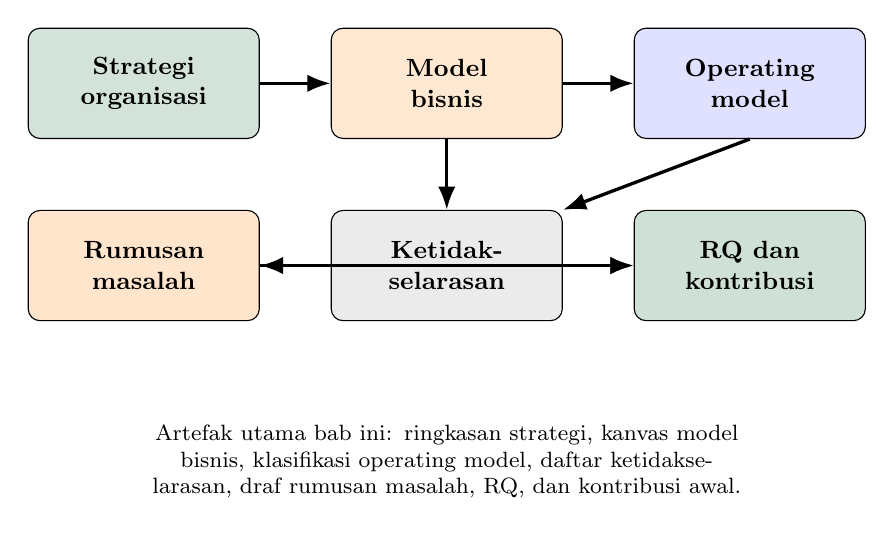
\begin{tikzpicture}[
  font=\small\bfseries,
  node distance=9mm,
  flowstep/.style={draw, rounded corners=1.5mm, align=center,
    minimum width=28mm, minimum height=14mm, text width=27mm},
  arrow/.style={-Latex, very thick}
]
  \node[flowstep, fill=praditagreen!20] (s) {Strategi\\organisasi};
  \node[flowstep, fill=orange!18, right=of s] (bmc) {Model\\bisnis};
  \node[flowstep, fill=blue!12, right=of bmc] (op) {Operating\\model};
  \node[flowstep, fill=gray!16, below=of bmc] (mis) {Ketidak-\\selarasan};
  \node[flowstep, fill=orange!20, left=of mis] (prob) {Rumusan\\masalah};
  \node[flowstep, fill=praditagreen!22, right=of mis] (rq) {RQ dan\\kontribusi};

  \draw[arrow] (s) -- (bmc);
  \draw[arrow] (bmc) -- (op);
  \draw[arrow] (op.south) -- (mis.north east);
  \draw[arrow] (bmc.south) -- (mis.north);
  \draw[arrow] (mis) -- (prob);
  \draw[arrow] (mis) -- (rq);
  \draw[arrow] (prob) -- (rq);

  \node[align=center, font=\footnotesize\mdseries, text width=96mm,
        below=12mm of mis]
    {Artefak utama bab ini: ringkasan strategi, kanvas model bisnis,
     klasifikasi operating model, daftar ketidakselarasan, draf rumusan
     masalah, RQ, dan kontribusi awal.};
\end{tikzpicture}
}
\caption{Alur berpikir Bab 2 dari strategi organisasi menuju pertanyaan
penelitian dan kontribusi makalah.}
\label{fig:strategi-ke-rq}
\end{figure}

Alur ini membantu mahasiswa menjaga fokus. Tanpa alur seperti ini, mahasiswa
sering melompat dari cerita organisasi ke rekomendasi teknologi. Padahal
makalah yang baik perlu memperlihatkan jejak penalaran: mengapa masalah itu
dipilih, mengapa penting, mengapa kerangka analisis tertentu dipakai, dan
mengapa rekomendasi yang muncul dapat dipertanggungjawabkan.

\section{Konteks Indonesia: Strategi Digital dalam Realitas Lokal}

Strategi digital organisasi Indonesia dibentuk oleh beberapa kondisi yang
perlu diperhatikan sejak awal. Pertama, kematangan digital antarorganisasi dan
antarwilayah tidak merata. Perusahaan besar di kota utama mungkin sudah
terbiasa dengan layanan berbasis API, sedangkan koperasi, BPR, rumah sakit
daerah, atau pemerintah kabupaten masih bergulat dengan integrasi dasar dan
kualitas data. Ketidakmerataan ini memengaruhi kelayakan rekomendasi.

Kedua, regulasi memberi batas dan arah. UU Pelindungan Data Pribadi menuntut
organisasi lebih berhati-hati dalam mengumpulkan, memproses, dan membagikan
data pribadi \cite{uupdp2022}. PP No.~71/2019 mengatur penyelenggaraan sistem
dan transaksi elektronik, termasuk tanggung jawab penyelenggara sistem
\cite{pp712019}. Di sektor pembayaran, SNAP BI dari Bank Indonesia memberi
standar integrasi API yang penting bagi organisasi keuangan dan fintech
\cite{snapbi}. Strategi yang tidak memperhitungkan regulasi dapat terlihat
menarik di atas kertas tetapi rapuh saat dijalankan.

Ketiga, banyak organisasi Indonesia bekerja dalam struktur yang hierarkis.
Keputusan digital sering tersentralisasi di kantor pusat, sementara
implementasi terjadi di cabang, unit layanan, atau mitra lapangan. Situasi ini
membuat operating model menjadi penting. Strategi digital yang menuntut
standardisasi tinggi membutuhkan mekanisme pelaksanaan yang berbeda dari
strategi yang memberi otonomi besar kepada unit lokal.

Keempat, biaya dan kapasitas SDM sering menjadi batas nyata. Mahasiswa tidak
boleh menulis rekomendasi seperti ``bangun platform nasional berbasis cloud
dan microservices'' tanpa menjelaskan prioritas, tahapan, risiko, dan
kesiapan organisasi. Dalam makalah, kepekaan terhadap konteks Indonesia bukan
hiasan; ia menentukan apakah analisis dapat dipercaya.

\section{Studi Kasus Utama: Menajamkan Masalah Bank Wanua}

Untuk melihat cara kerja bab ini, kita kembali ke Bank Wanua. Strategi awal
bank adalah menjadi mitra digital UMKM daerah. Strategi ini dapat dipetakan
ke dalam beberapa elemen kanvas model bisnis sebagaimana Tabel~\ref{tab:bank-wanua-bmc}.

\begin{table}[htbp]
\centering
\scriptsize
\caption{Ringkasan model bisnis Bank Wanua untuk strategi UMKM digital.}
\label{tab:bank-wanua-bmc}
\begin{tabularx}{\textwidth}{@{}p{0.24\textwidth} X X@{}}
\hline
\textbf{Elemen} & \textbf{Kondisi Saat Ini} & \textbf{Arah Strategis} \\
\hline
Segmen pelanggan & Nasabah ritel lokal, pegawai daerah, pelaku UMKM lama. &
UMKM yang membutuhkan layanan pembayaran, pembiayaan, dan pencatatan transaksi
digital. \\
Proposisi nilai & Kedekatan lokal dan layanan cabang. & Layanan keuangan
terintegrasi untuk UMKM: rekening, pembayaran, pembiayaan, dan akses mitra. \\
Kanal & Cabang, agen, ATM, aplikasi mobile dasar. & Mobile banking, API mitra,
QRIS, dan kanal cabang sebagai pendamping digital. \\
Aktivitas kunci & Pembukaan rekening, transaksi, kredit, layanan cabang. &
Onboarding digital UMKM, integrasi pembayaran, analitik risiko sederhana,
tata kelola mitra API. \\
Mitra kunci & Pemerintah daerah, koperasi, komunitas UMKM. & Fintech,
marketplace lokal, koperasi, penyedia layanan pembayaran, pemerintah daerah. \\
\hline
\end{tabularx}
\end{table}

Dari tabel tersebut terlihat bahwa strategi baru menuntut koordinasi data dan
standardisasi proses yang lebih tinggi. Bank Wanua tidak cukup hanya menambah
fitur aplikasi. Ia perlu memastikan data nasabah UMKM dapat dibaca lintas
kanal, proses pembukaan rekening dan verifikasi risiko cukup konsisten, dan
aturan berbagi data dengan mitra dipahami sejak awal. Dengan kata lain, Bank
Wanua bergerak dari model operasi yang cenderung cabang-sentris menuju model
yang lebih terkoordinasi.

Ketidakselarasan yang muncul dapat diringkas sebagai berikut:

\begin{enumerate}
  \item \textbf{Strategi pelanggan tidak selaras dengan data.} Bank ingin
        memahami UMKM secara lebih baik, tetapi data nasabah, transaksi, dan
        interaksi cabang belum menjadi satu pandangan yang konsisten.
  \item \textbf{Strategi kemitraan tidak selaras dengan tata kelola API.} Bank
        ingin terhubung dengan mitra, tetapi belum memiliki prioritas layanan
        API, kriteria mitra, dan mekanisme pengawasan.
  \item \textbf{Strategi efisiensi tidak selaras dengan proses cabang.} Bank
        ingin mempercepat layanan, tetapi proses verifikasi dan persetujuan
        masih berbeda antarcabang.
  \item \textbf{Strategi personalisasi tidak selaras dengan kepatuhan data.}
        Bank ingin memberi penawaran yang lebih personal, tetapi belum
        menjelaskan batas penggunaan data pribadi dan persetujuan nasabah.
\end{enumerate}

Dari sini, rumusan masalah awal dapat ditulis:

\begin{quote}
Strategi Bank Wanua untuk menjadi mitra digital UMKM daerah belum didukung
oleh model operasi dan arah arsitektur enterprise yang jelas. Ketidakselarasan
terlihat pada integrasi data nasabah UMKM, standardisasi proses lintas cabang,
prioritas layanan API untuk mitra, dan tata kelola penggunaan data pribadi.
Kondisi ini menyulitkan bank untuk menerjemahkan ambisi digital menjadi
kapabilitas yang dapat dijalankan secara bertahap dan sesuai konteks regulasi
Indonesia.
\end{quote}

Rumusan tersebut dapat diubah menjadi RQ awal:

\begin{quote}
Bagaimana pendekatan Enterprise Architecture berbasis TOGAF-lite dan BDAT
dapat digunakan untuk merumuskan arah arsitektur target yang menyelaraskan
strategi Bank Wanua sebagai mitra digital UMKM dengan kebutuhan integrasi data,
standardisasi proses, layanan API, dan tata kelola data pribadi?
\end{quote}

Kontribusi awal makalah dapat ditulis:

\begin{quote}
Makalah ini menawarkan analisis studi kasus Bank Wanua dengan memetakan
ketidakselarasan antara strategi bisnis dan kapabilitas arsitektur enterprise.
Kontribusi praktisnya adalah rancangan awal arah BDAT, prioritas API, dan
prinsip tata kelola yang realistis untuk bank daerah di Indonesia. Kontribusi
akademiknya adalah contoh penerapan TOGAF-lite untuk menjembatani strategi
UMKM digital, operating model, dan konteks regulasi lokal.
\end{quote}

Contoh ini belum sempurna, tetapi sudah cukup untuk menjadi dasar konsultasi.
Pada bab-bab berikutnya, RQ tersebut dapat dipersempit lagi sesuai data yang
tersedia dan target publikasi yang dipilih.

\section{Langkah Analisis dan Artefak Pendukung}

Gunakan delapan langkah berikut untuk mengubah topik awal menjadi rumusan
masalah, RQ, dan kontribusi awal.

\begin{enumerate}
  \item \textbf{Tulis ulang strategi organisasi dalam satu paragraf.} Hindari
        slogan. Sebutkan pelanggan, nilai, kanal, dan prioritas.
  \item \textbf{Petakan model bisnis secara ringkas.} Gunakan komponen kanvas
        model bisnis yang paling relevan. Tidak semua komponen harus sama
        panjang.
  \item \textbf{Tentukan operating model yang paling mendekati.} Apakah
        organisasi membutuhkan integrasi data tinggi, standardisasi proses
        tinggi, keduanya, atau justru otonomi unit?
  \item \textbf{Daftar ketidakselarasan utama.} Cari jarak antara strategi dan
        kondisi proses, data, aplikasi, teknologi, API, atau tata kelola.
  \item \textbf{Pilih satu ketidakselarasan utama.} Makalah satu semester
        sebaiknya tidak mencoba menjawab semua masalah sekaligus.
  \item \textbf{Tulis rumusan masalah 1--2 paragraf.} Jelaskan konteks,
        ketegangan, dampak, dan mengapa masalah ini penting dianalisis.
  \item \textbf{Ubah menjadi RQ.} Gunakan bentuk tanya yang dapat dijawab
        dengan analisis, bukan pertanyaan yang jawabannya sekadar ya atau
        tidak.
  \item \textbf{Tulis kontribusi awal.} Bedakan kontribusi praktis bagi
        organisasi dan kontribusi akademik bagi pembaca makalah.
\end{enumerate}

Tabel~\ref{tab:rq-baik-buruk} memberi contoh perbaikan RQ.

\begin{table}[htbp]
\centering
\scriptsize
\caption{Contoh memperbaiki pertanyaan penelitian.}
\label{tab:rq-baik-buruk}
\begin{tabularx}{\textwidth}{@{}p{0.30\textwidth} X X@{}}
\hline
\textbf{Versi Lemah} & \textbf{Masalahnya} & \textbf{Versi Lebih Kuat} \\
\hline
Bagaimana membuat aplikasi mobile Bank Wanua? & Terlalu teknis dan langsung
melompat ke solusi. & Bagaimana arsitektur aplikasi dan data Bank Wanua perlu
diselaraskan untuk mendukung layanan digital UMKM lintas kanal? \\
Apakah API penting bagi bank daerah? & Jawabannya terlalu umum dan mudah
ditebak. & Layanan API apa yang sebaiknya diprioritaskan bank daerah untuk
mendukung kemitraan UMKM, dan risiko tata kelola apa yang perlu dikendalikan? \\
Bagaimana transformasi digital rumah sakit? & Terlalu luas untuk satu makalah.
& Bagaimana rumah sakit daerah dapat menyelaraskan proses pendaftaran, data
pasien, dan kanal telekonsultasi dalam arsitektur target yang sesuai regulasi
data pribadi? \\
\hline
\end{tabularx}
\end{table}

\subsection*{Artefak Pendukung Bab Ini}

Bab ini menghasilkan artefak ringan, tetapi penting. Artefak tersebut tidak
dinilai sebagai luaran terpisah; fungsinya adalah memperkuat argumen awal
makalah.

\begin{table}[htbp]
\centering
\scriptsize
\caption{Artefak Bab 2 dan fungsi akademiknya.}
\label{tab:artefak-bab2}
\begin{tabularx}{\textwidth}{@{}p{0.26\textwidth} X X@{}}
\hline
\textbf{Artefak} & \textbf{Fungsi Analisis} & \textbf{Masuk ke Makalah Sebagai} \\
\hline
Ringkasan strategi & Menjelaskan arah organisasi dan prioritas transformasi. &
Latar belakang pada Pendahuluan. \\
Kanvas model bisnis ringkas & Menghubungkan pelanggan, nilai, aktivitas,
sumber daya, dan mitra. & Konteks organisasi atau lampiran ringkas. \\
Klasifikasi operating model & Menjelaskan kebutuhan standardisasi proses dan
integrasi data. & Justifikasi masalah dan metode analisis. \\
Daftar ketidakselarasan & Menunjukkan jarak antara strategi dan kapabilitas
saat ini. & Bukti awal rumusan masalah. \\
Draf RQ dan kontribusi & Mengarahkan struktur analisis semester berjalan. &
Bagian akhir Pendahuluan. \\
\hline
\end{tabularx}
\end{table}

Artefak yang baik harus relevan dengan RQ, mudah dipahami pembaca non-IT,
menunjukkan sebab-akibat atau prioritas, konsisten dengan narasi makalah, dan
menyebutkan sumber data atau asumsi yang digunakan.

\section{Integrasi ke Makalah Publikasi}

Bab ini terutama memperkuat bagian \textbf{Pendahuluan} makalah. Setelah
menyelesaikan bab ini, mahasiswa seharusnya memiliki empat bahan yang langsung
dapat dipindahkan ke naskah:

\begin{enumerate}
  \item satu paragraf konteks organisasi dan strategi digital;
  \item satu paragraf rumusan masalah;
  \item satu atau dua RQ yang dapat dijawab melalui analisis;
  \item satu paragraf kontribusi awal.
\end{enumerate}

Keempat bahan ini juga menjadi dasar bagian \textbf{Metode} dan
\textbf{Analisis} pada bab-bab berikutnya. RQ menentukan data apa yang perlu
dikumpulkan, kerangka apa yang dipakai, dan artefak apa yang harus dibuat. Jika
RQ menekankan integrasi data, Bab 5 akan menjadi sangat penting. Jika RQ
menekankan layanan API, Bab 9 dan Bab 10 perlu mendapat porsi lebih besar. Jika
RQ menekankan platform, Bab 11 dan Bab 12 akan menjadi inti diskusi.

Ingat bahwa kontribusi awal masih boleh berubah. Pada tahap ini, kontribusi
berfungsi sebagai arah kerja. Setelah literatur dibaca dan analisis kasus
dilakukan, kontribusi dapat dipertajam menjadi lebih spesifik.

\subsection*{Contoh Paragraf Akademik}

Contoh berikut menunjukkan cara mengubah artefak Bab 2 menjadi narasi
Pendahuluan:

\begin{quote}
Organisasi studi kasus menunjukkan ketidakselarasan antara ambisi digital dan
model operasi yang tersedia. Meskipun strategi organisasi menekankan layanan
digital lintas kanal, proses inti masih berjalan berbeda antarunit, sementara
data pelanggan belum memiliki definisi dan kepemilikan yang konsisten. Kondisi
ini menunjukkan bahwa masalah utama bukan sekadar keterbatasan aplikasi,
melainkan belum tersedianya arah arsitektur enterprise yang menghubungkan
strategi, integrasi data, standardisasi proses, dan tata kelola. Oleh karena
itu, penelitian ini mengajukan pertanyaan bagaimana pendekatan Enterprise
Architecture dapat digunakan untuk menyelaraskan strategi digital organisasi
dengan kapabilitas bisnis dan teknologi yang realistis dalam konteks Indonesia.
\end{quote}

\section{Diskusi Kritis dan Perangkap Umum}

Beberapa perangkap berikut sering terjadi ketika mahasiswa merumuskan masalah
penelitian.

\begin{enumerate}
  \item \textbf{Masalah terlalu luas.} ``Transformasi digital sektor kesehatan
        Indonesia'' tidak cocok untuk makalah satu semester. Persempit menjadi
        organisasi, proses, kapabilitas, atau keputusan tertentu.
  \item \textbf{Masalah terlalu teknis.} ``Implementasi REST API'' belum tentu
        menjadi masalah EA. Jelaskan nilai bisnis, mitra, tata kelola, dan
        risiko yang membuat API itu penting.
  \item \textbf{RQ tidak dapat dijawab dengan data yang tersedia.} Jika
        mahasiswa tidak punya akses ke data internal, pilih pendekatan yang
        mengandalkan dokumen publik, wawancara terbatas, atau kajian
        konseptual berbasis kasus.
  \item \textbf{Kontribusi terdengar seperti janji konsultan.} Kalimat seperti
        ``meningkatkan efisiensi 50\%'' perlu bukti. Untuk makalah awal,
        kontribusi yang lebih aman adalah kerangka analisis, rancangan awal,
        atau rekomendasi berbasis bukti.
  \item \textbf{Mengabaikan target publikasi.} Target publikasi memengaruhi
        panjang, gaya sitasi, jumlah referensi, dan kedalaman metode. RQ harus
        cukup cocok dengan ruang lingkup target publikasi.
  \item \textbf{Tidak membedakan gejala dan masalah.} Aplikasi lambat,
        data ganda, atau proses manual sering hanya gejala. Masalah yang lebih
        dalam mungkin terletak pada model operasi, kepemilikan data, atau
        prioritas strategi.
\end{enumerate}

Trade-off utama pada bab ini adalah antara keluasan dan ketajaman. Rumusan
yang terlalu sempit mudah dianalisis tetapi mungkin kurang bernilai akademik.
Rumusan yang terlalu luas terdengar penting tetapi sulit diselesaikan. Pilih
masalah yang cukup kecil untuk ditangani, tetapi cukup penting untuk
dipublikasikan.

\begin{table}[htbp]
\centering
\scriptsize
\caption{Trade-off saat merumuskan masalah dan RQ.}
\label{tab:tradeoff-rq}
\begin{tabularx}{\textwidth}{@{}p{0.22\textwidth} X X X@{}}
\hline
\textbf{Keputusan} & \textbf{Manfaat} & \textbf{Risiko} & \textbf{Prioritas} \\
\hline
RQ sangat sempit & Analisis lebih mudah dikendalikan. & Kontribusi dapat
terlihat terlalu kecil. & Cocok bila data terbatas dan target publikasi
praktis. \\
RQ luas lintas domain & Kontribusi terasa strategis. & Sulit selesai dalam
satu semester. & Hanya dipilih jika data dan literatur cukup kuat. \\
Fokus pada teknologi & Artefak teknis lebih jelas. & Argumen manajerial
melemah. & Perlu selalu dikaitkan dengan strategi dan risiko. \\
Fokus pada tata kelola & Relevan bagi manajemen dan regulasi. & Butuh bukti
tentang peran, proses, dan keputusan. & Cocok untuk organisasi yang datanya
sensitif atau bermitra luas. \\
\hline
\end{tabularx}
\end{table}

\section{Latihan Terapan Individual}

\subsection*{Latihan~2.1: Ringkasan Strategi dan Model Bisnis}

Gunakan organisasi studi kasus yang sudah dipilih pada Bab~\ref{ch:orientasi}.
Tuliskan ringkasan satu sampai dua halaman yang memuat:

\begin{enumerate}
  \item strategi digital organisasi dalam satu paragraf;
  \item tiga segmen pengguna atau pemangku kepentingan utama;
  \item proposisi nilai yang dijanjikan kepada masing-masing segmen;
  \item aktivitas kunci, sumber daya kunci, dan mitra kunci;
  \item satu masalah strategis yang paling tampak dari peta tersebut.
\end{enumerate}

\subsection*{Latihan~2.2: Klasifikasi Operating Model}

Nilailah organisasi Anda menggunakan dua pertanyaan:

\begin{enumerate}
  \item Seberapa tinggi kebutuhan standardisasi proses?
  \item Seberapa tinggi kebutuhan integrasi data?
\end{enumerate}

Pilih salah satu pola operating model: \emph{Diversification},
\emph{Coordination}, \emph{Replication}, atau \emph{Unification}. Jelaskan
alasan pemilihan tersebut dalam 2--3 paragraf. Jika organisasi Anda berada di
antara dua pola, jelaskan ketegangan yang muncul.

\subsection*{Latihan~2.3: Draf Rumusan Masalah, RQ, dan Kontribusi}

Susun draf awal dengan format berikut:

\begin{enumerate}
  \item Rumusan masalah: 1--2 paragraf.
  \item RQ utama: satu pertanyaan.
  \item Sub-RQ opsional: maksimum dua pertanyaan.
  \item Kontribusi praktis: 2--3 kalimat.
  \item Kontribusi akademik: 2--3 kalimat.
\end{enumerate}

Pastikan RQ tidak langsung melompat ke solusi. RQ yang baik membuka ruang
analisis, bukan sekadar meminta pembaca menyetujui teknologi tertentu.

\subsection*{Latihan~2.4: Uji Kelayakan Target Publikasi}

Ambil satu target publikasi dari daftar Bab~\ref{ch:orientasi}. Periksa apakah
rumusan masalah dan RQ Anda cocok dengan ruang lingkup target tersebut.
Tuliskan catatan singkat:

\begin{itemize}
  \item bagian ruang lingkup target publikasi yang paling relevan;
  \item tipe artikel yang paling cocok;
  \item panjang naskah atau batas halaman;
  \item konsekuensi bagi struktur RQ dan metode.
\end{itemize}

\subsection*{Rubrik Mini Latihan}

\begin{table}[htbp]
\centering
\scriptsize
\caption{Rubrik mini untuk keluaran latihan Bab 2.}
\label{tab:rubrik-latihan-bab2}
\begin{tabularx}{\textwidth}{@{}p{0.26\textwidth} X@{}}
\hline
\textbf{Kriteria} & \textbf{Indikator Kualitas} \\
\hline
Relevansi masalah & Masalah berasal dari strategi organisasi, bukan sekadar
ketertarikan pada teknologi tertentu. \\
Ketepatan konsep & Kanvas model bisnis dan operating model digunakan secara
tepat untuk menjelaskan ketidakselarasan. \\
Kejelasan artefak & Ringkasan strategi, klasifikasi operating model, dan
daftar ketidakselarasan mudah dibaca audiens non-IT. \\
Kekuatan argumen & Rumusan masalah menunjukkan konteks, bukti awal, dampak,
dan urgensi akademik/praktis. \\
Kelayakan implementasi & RQ dapat dijawab dengan data, waktu, dan kapasitas
yang tersedia dalam satu semester. \\
Keterhubungan ke makalah & Kontribusi awal jelas masuk ke bagian Pendahuluan
dan memberi arah bagi metode serta analisis. \\
\hline
\end{tabularx}
\end{table}

\subsection*{Pertanyaan Refleksi}

\begin{enumerate}
  \item Apakah masalah yang Anda pilih berasal dari strategi organisasi atau
        hanya dari ketertarikan pada teknologi tertentu?
  \item Apakah RQ Anda dapat dijawab dengan data dan waktu yang tersedia dalam
        satu semester?
  \item Apa risiko terbesar jika organisasi mengikuti rekomendasi yang mungkin
        muncul dari makalah Anda?
  \item Bagian mana yang perlu dikonsultasikan dengan dosen sebelum masuk ke
        Bab 3?
\end{enumerate}

\section{Ringkasan, Refleksi, dan Jembatan}

\subsection*{Poin Kunci}

\begin{itemize}
  \item Strategi bisnis harus dibaca sebagai pilihan tentang pelanggan,
        proposisi nilai, prioritas, dan cara organisasi menciptakan nilai.
  \item Kanvas model bisnis membantu menghubungkan strategi dengan aktivitas,
        sumber daya, mitra, kanal, dan struktur biaya.
  \item Operating model membantu membaca kebutuhan standardisasi proses dan
        integrasi data.
  \item Rumusan masalah yang baik menjelaskan ketegangan, bukti awal, dampak,
        dan konteks.
  \item RQ harus dapat dijawab melalui analisis, bukan sekadar menyatakan
        solusi yang sudah dipilih sejak awal.
  \item Kontribusi awal perlu membedakan nilai praktis bagi organisasi dan
        nilai akademik bagi pembaca makalah.
\end{itemize}

\subsection*{Jawaban Ringkas atas Pertanyaan Pemandu}

\begin{enumerate}
  \item Strategi organisasi dibaca dari pelanggan prioritas, nilai yang
        dijanjikan, kanal, aktivitas kunci, dan mitra kunci.
  \item Model bisnis menunjukkan bagaimana organisasi menghasilkan nilai,
        sedangkan operating model menunjukkan bagaimana nilai itu dijalankan
        melalui proses dan data.
  \item Ketidakselarasan muncul ketika strategi menuntut kapabilitas yang
        belum didukung proses, data, aplikasi, teknologi, API, atau tata
        kelola.
  \item Bukti awal dapat berupa dokumen publik, proses yang diamati, wawancara,
        laporan tahunan, regulasi, atau artefak internal yang diizinkan.
  \item Hasil analisis menjadi argumen akademik ketika artefak dipakai untuk
        mendukung klaim, bukan hanya ditempel sebagai gambar.
\end{enumerate}

\subsection*{Uji Mandiri: Pertanyaan Konseptual}

\begin{enumerate}
  \item Mengapa strategi bisnis perlu dibaca sebelum menyusun arsitektur
        enterprise?
  \item Jelaskan perbedaan antara strategi bisnis dan model bisnis.
  \item Apa fungsi operating model dalam analisis Enterprise Architecture?
  \item Sebutkan dua dimensi utama operating model dan jelaskan artinya.
  \item Apa perbedaan antara rumusan masalah, RQ, dan pernyataan kontribusi?
  \item Mengapa RQ yang terlalu teknis dapat melemahkan makalah Enterprise
        Architecture?
\end{enumerate}

\subsection*{Pertanyaan Aplikatif}

\begin{enumerate}
  \item Sebuah universitas ingin membangun layanan akademik terpadu. Mahasiswa,
        dosen, keuangan, dan administrasi memakai aplikasi berbeda. Rumuskan
        satu masalah penelitian yang lebih tajam daripada ``sistem belum
        terintegrasi''.
  \item Sebuah koperasi ingin menjual produk anggotanya melalui marketplace
        lokal. Pilih operating model yang paling mendekati dan jelaskan
        alasannya.
  \item Sebuah rumah sakit daerah ingin memperluas telekonsultasi, tetapi data
        pasien tersebar antara unit pendaftaran, poli, laboratorium, dan
        farmasi. Buat satu RQ yang menghubungkan strategi layanan digital dan
        arsitektur data.
\end{enumerate}

\subsection*{Pertanyaan Reflektif untuk Makalah}

\begin{enumerate}
  \item Apakah RQ Anda lebih dekat dengan domain Business, Data, Application,
        Technology, API, atau platform? Apa konsekuensinya bagi bab-bab
        berikutnya?
  \item Apakah kontribusi yang Anda tulis lebih kuat sebagai kontribusi
        praktis, akademik, atau keduanya? Mengapa?
\end{enumerate}

\subsection*{Ringkasan Naratif}

Bab ini menunjukkan bahwa rumusan masalah makalah tidak boleh muncul dari
ketertarikan teknologi semata. Rumusan yang baik berangkat dari strategi
organisasi, model bisnis, model operasi, dan ketidakselarasan yang dapat
dibuktikan. Kanvas model bisnis membantu pembaca melihat bagaimana organisasi
menciptakan nilai, sedangkan operating model membantu membaca kebutuhan
standardisasi proses dan integrasi data.

Dalam konteks Indonesia, strategi digital harus mempertimbangkan kematangan
organisasi yang beragam, regulasi seperti UU PDP dan PP No.~71/2019,
ketentuan sektor seperti SNAP BI, struktur organisasi yang sering hierarkis,
serta keterbatasan biaya dan SDM. Kepekaan terhadap konteks ini membuat RQ
lebih realistis dan kontribusi lebih dapat dipercaya.

Keluaran utama bab ini adalah draf rumusan masalah, RQ, dan kontribusi awal.
Ketiganya akan menjadi kompas bagi bab-bab berikutnya. Jika kompas ini kabur,
artefak arsitektur yang dibuat pada Bab 3 sampai Bab 12 akan mudah menjadi
kumpulan gambar yang tidak menyatu dengan argumen makalah.

\subsection*{Jembatan ke Bab Berikutnya}

Bab berikutnya memperkenalkan TOGAF-lite dan cara menyusun tinjauan pustaka
awal. Setelah strategi dan RQ mulai jelas, pembaca perlu memilih kerangka
analisis yang dapat dipertanggungjawabkan. TOGAF-lite akan dipakai sebagai
bahasa kerja untuk menyusun visi arsitektur, kondisi saat ini, arsitektur
target, analisis kesenjangan, dan peta jalan. Pada saat yang sama, mahasiswa
mulai membangun bibliografi awal agar rumusan masalah tidak hanya kuat secara
praktis, tetapi juga tersambung dengan percakapan akademik.

\section{Bacaan Lanjutan}

\subsection*{Bacaan Inti}

\begin{itemize}
  \item \emph{Enterprise Architecture as Strategy}~\cite{ross2006enterprise}.
        Rujukan utama untuk memahami operating model dan hubungan strategi
        bisnis dengan fondasi arsitektur.
  \item \emph{Designed for Digital}~\cite{ross2019designed}. Membantu pembaca
        memahami kapabilitas organisasi digital dan mengapa strategi perlu
        diterjemahkan menjadi kemampuan yang dapat dijalankan.
  \item \emph{TOGAF Standard, 10th Edition}~\cite{togaf10}. Bacaan awal untuk
        melihat bagaimana visi arsitektur dan kebutuhan bisnis ditempatkan
        dalam siklus pengembangan arsitektur.
\end{itemize}

\subsection*{Bacaan untuk Memperdalam}

\begin{itemize}
  \item \emph{Platform Revolution}~\cite{parker2016platform}. Berguna bagi
        mahasiswa yang rumusan masalahnya mengarah ke ekosistem platform dan
        \emph{network effects}.
  \item \emph{The Business of Platforms}~\cite{cusumano2019business}. Cocok
        untuk memperdalam diskusi tentang strategi dan tata kelola model
        bisnis platform.
  \item \emph{APIs: A Strategy Guide}~\cite{jacobson2011apis}. Bermanfaat jika
        ketidakselarasan utama organisasi berkaitan dengan kemitraan API,
        integrasi layanan, atau pembukaan kanal digital untuk pihak luar.
\end{itemize}

\subsection*{Sumber Indonesia}

\begin{itemize}
  \item \emph{Undang-Undang Pelindungan Data Pribadi}~\cite{uupdp2022}.
        Penting untuk mahasiswa yang rumusan masalahnya menyentuh data
        pelanggan, personalisasi layanan, atau integrasi data lintas kanal.
  \item \emph{PP No.~71/2019}~\cite{pp712019}. Relevan untuk memahami
        tanggung jawab penyelenggara sistem elektronik.
  \item \emph{Standar Nasional Open API Pembayaran (SNAP BI)}~\cite{snapbi}.
        Sangat relevan untuk topik open banking, fintech, pembayaran digital,
        dan API sektor keuangan.
\end{itemize}

\subsection*{Lampiran: Worksheet Ringkas Bab 2}

Gunakan format berikut sebagai catatan kerja sebelum menulis bagian
Pendahuluan makalah.

\begin{enumerate}
  \item \textbf{Strategi organisasi:} tuliskan 4--6 kalimat tentang pelanggan,
        nilai, kanal, prioritas, dan batasan utama.
  \item \textbf{Model bisnis:} rangkum segmen pelanggan, proposisi nilai,
        aktivitas kunci, sumber daya kunci, dan mitra kunci.
  \item \textbf{Operating model:} pilih salah satu pola dan jelaskan alasan
        berdasarkan kebutuhan standardisasi proses dan integrasi data.
  \item \textbf{Ketidakselarasan utama:} tuliskan tiga jarak paling penting
        antara strategi dan kondisi saat ini.
  \item \textbf{Rumusan masalah:} tulis 1--2 paragraf yang menjelaskan konteks,
        ketegangan, dampak, dan pentingnya analisis.
  \item \textbf{RQ dan kontribusi:} tulis satu RQ utama, maksimum dua sub-RQ,
        kontribusi praktis, dan kontribusi akademik.
\end{enumerate}

    \chapter[TOGAF-lite, ADM, dan Tinjauan Pustaka]{TOGAF-lite, ADM, dan Tinjauan Pustaka: Menyusun Visi Arsitektur dan Fondasi Akademik}
\label{ch:togaf-lite}
\setlength{\emergencystretch}{2em}

\section*{Tujuan Pembelajaran}
\begin{itemize}
  \item Menjelaskan fungsi TOGAF-lite dan ADM sebagai kerangka kerja ringan
        untuk menata perubahan arsitektur enterprise.
  \item Menyusun visi arsitektur awal yang berangkat dari masalah, pertanyaan
        riset, pemangku kepentingan, dan batasan organisasi.
  \item Merancang strategi pencarian pustaka dan bibliografi awal yang relevan
        dengan topik makalah individual.
  \item Menghubungkan sintesis pustaka, visi arsitektur, dan metode
        TOGAF-lite ke dalam rancangan awal makalah publikasi.
\end{itemize}

Bab ini terutama mendukung capaian pembelajaran yang berkaitan dengan
pemahaman konsep arsitektur enterprise, analisis pemangku kepentingan,
penyusunan argumen berbasis pustaka, dan penyiapan naskah publikasi
individual.

\section{Ringkasan Awal Bab}

Bab sebelumnya membantu pembaca memilih topik, merumuskan masalah, dan
membentuk pertanyaan riset awal. Bab ini mengubah rumusan tersebut menjadi
dua fondasi yang dapat dikerjakan secara terstruktur: visi arsitektur dan
tinjauan pustaka awal. Visi arsitektur menjelaskan arah perubahan yang ingin
dibahas dalam makalah. Tinjauan pustaka memberi dasar akademik agar arah
perubahan tersebut tidak hanya menjadi opini pribadi, melainkan berdiri di
atas konsep, temuan, standar, dan pengalaman yang sudah pernah dibahas dalam
literatur.

TOGAF digunakan secara ringan, bukan sebagai prosedur birokratis penuh. Yang
diambil adalah cara berpikir ADM: memahami konteks, merumuskan visi,
memetakan kondisi saat ini, membayangkan kondisi target, menemukan
kesenjangan, lalu menyusun arah perubahan. Dalam konteks mata kuliah ini, ADM
menjadi alat bantu untuk menulis makalah yang lebih rapi: masalahnya jelas,
kerangka konseptualnya terlihat, metode analisisnya dapat dijelaskan, dan
rekomendasinya dapat ditelusuri kembali ke bukti.

Pada akhir bab, setiap mahasiswa menghasilkan visi arsitektur satu halaman,
strategi pencarian pustaka, bibliografi awal minimal sepuluh rujukan, dan
kerangka metode singkat untuk makalah individual.

\section{Pendahuluan}

Makalah publikasi membutuhkan dua hal yang sering tertukar. Pertama, ia perlu
arah perubahan yang jelas. Kedua, ia perlu dasar pustaka yang cukup untuk
menunjukkan bahwa penulis memahami percakapan ilmiah dan profesional di
bidangnya. Jika hanya ada arah perubahan, naskah mudah berubah menjadi
proposal internal. Jika hanya ada pustaka, naskah mudah menjadi rangkuman
artikel tanpa kontribusi.

Bab ini mempertemukan keduanya. TOGAF-lite dipakai untuk menyusun arah
perubahan melalui visi arsitektur. Tinjauan pustaka dipakai untuk membangun
argumen, memilih konsep, dan menjelaskan mengapa usulan perubahan tersebut
layak dibahas. Dengan begitu, mahasiswa tidak sekadar menulis bahwa organisasi
perlu ``bertransformasi digital'', tetapi dapat menunjukkan perubahan apa yang
dibahas, bukti apa yang mendukung, dan bagaimana analisis dilakukan.

Pendekatan ini sesuai dengan keluaran utama mata kuliah: satu makalah
individual yang siap dikembangkan untuk jurnal atau konferensi. Artefak
arsitektur tetap dibuat, tetapi posisinya sebagai penguat naskah. Artefak
yang baik membantu penulis berpikir dan membantu pembaca memahami argumen.

\section{Skenario Pembuka dan Pertanyaan Pemandu}

Tim pengembangan layanan digital Bank Wanua mulai menyadari bahwa persoalan
mereka bukan sekadar aplikasi yang lambat atau data nasabah yang tersebar.
Masalah yang lebih besar adalah tidak adanya gambaran bersama tentang arah
perubahan. Unit bisnis ingin layanan baru cepat diluncurkan. Unit kepatuhan
menuntut tata kelola data yang lebih kuat. Tim teknologi ingin mengurangi
ketergantungan pada sistem lama. Pimpinan meminta satu dokumen ringkas yang
menjelaskan perubahan apa yang akan dilakukan, mengapa perubahan itu penting,
dan dasar akademik apa yang mendukung pilihan tersebut.

Seorang mahasiswa yang memilih kasus Bank Wanua sebagai topik makalah
menghadapi pertanyaan serupa. Ia sudah memiliki isu awal, misalnya integrasi
layanan digital, tata kelola data, atau modernisasi API. Namun, ia belum tahu
bagaimana menjadikan isu itu sebagai makalah yang layak dipublikasikan. Jika
hanya menulis deskripsi masalah, naskah akan terasa seperti laporan internal.
Jika hanya mengutip banyak artikel, naskah akan kehilangan arah praktis. Bab
ini membantu menautkan keduanya: arah perubahan dirumuskan melalui visi
arsitektur, sedangkan dasar akademiknya dibangun melalui tinjauan pustaka.

\subsection*{Pertanyaan Pemandu}

\begin{enumerate}
  \item Perubahan arsitektur apa yang benar-benar ingin dijelaskan dalam
        makalah?
  \item Siapa pemangku kepentingan utama, dan kekhawatiran apa yang perlu
        dijawab?
  \item Bagaimana ADM dapat disederhanakan agar cocok untuk analisis akademik
        individual?
  \item Literatur apa yang diperlukan agar argumen makalah tidak berdiri di
        atas asumsi pribadi?
  \item Bagaimana visi arsitektur dan tinjauan pustaka dapat menyatu dalam
        metode penulisan makalah?
\end{enumerate}

\section{Mengapa Bab Ini Penting}

Mahasiswa non-TI sering kali sudah memahami masalah organisasi dengan baik,
tetapi belum tentu terbiasa mengubah masalah tersebut menjadi argumen akademik
yang sistematis. Sebaliknya, mahasiswa juga dapat mengumpulkan banyak artikel
tanpa benar-benar tahu bagaimana artikel itu akan dipakai dalam analisis.
Keduanya berisiko menghasilkan naskah yang dangkal: kaya kutipan tetapi miskin
arah, atau kaya pengalaman tetapi lemah dasar ilmiah.

TOGAF-lite membantu mahasiswa menata arah perubahan. Tinjauan pustaka
membantu mahasiswa menata dasar pengetahuan. Keduanya perlu berjalan bersama.
Visi arsitektur tanpa pustaka dapat berubah menjadi klaim normatif. Tinjauan
pustaka tanpa visi arsitektur dapat berubah menjadi daftar ringkasan artikel.
Makalah publikasi membutuhkan keduanya: fokus perubahan yang tajam dan argumen
yang dapat dipertanggungjawabkan.

\section{Konsep Inti dan Glosarium Mini}

\subsection{TOGAF-lite}

TOGAF adalah kerangka kerja arsitektur enterprise yang menyediakan konsep,
siklus kerja, dan artefak untuk mengelola perubahan arsitektur organisasi
\cite{togaf10}. Dalam praktik profesional, TOGAF dapat digunakan secara luas
dan formal. Dalam mata kuliah ini, TOGAF digunakan secara ringan. Istilah
``TOGAF-lite'' berarti mahasiswa tidak diminta meniru seluruh dokumentasi
TOGAF, melainkan mengambil pola berpikir yang paling berguna untuk makalah:
memahami konteks, menyatakan visi, membandingkan kondisi saat ini dan kondisi
target, lalu menyusun rekomendasi perubahan.

Pendekatan ringan ini penting karena keluaran utama mata kuliah adalah makalah
individual, bukan proyek implementasi besar. Artefak arsitektur tetap dibuat,
tetapi posisinya sebagai alat bantu analisis. Artefak tersebut harus
memperjelas argumen naskah, bukan menjadi tumpukan lampiran yang terpisah dari
tulisan.

\subsection{ADM sebagai Siklus Berpikir}

Architecture Development Method atau ADM adalah bagian penting dari TOGAF. ADM
menggambarkan proses pengembangan arsitektur secara bertahap, mulai dari
persiapan, visi, arsitektur bisnis, sistem informasi, teknologi, peluang dan
solusi, perencanaan migrasi, implementasi, hingga tata kelola perubahan
\cite{togaf10}. Untuk kebutuhan makalah individual, ADM dapat disederhanakan
menjadi enam pertanyaan:

\begin{enumerate}
  \item Apa masalah dan pertanyaan risetnya?
  \item Apa visi arsitektur yang ingin dicapai?
  \item Bagaimana kondisi saat ini?
  \item Seperti apa kondisi target yang masuk akal?
  \item Kesenjangan apa yang perlu dijembatani?
  \item Rekomendasi perubahan apa yang paling layak dipertahankan secara
        akademik?
\end{enumerate}

\begin{figure}[htbp]
\centering
\scalebox{0.88}{
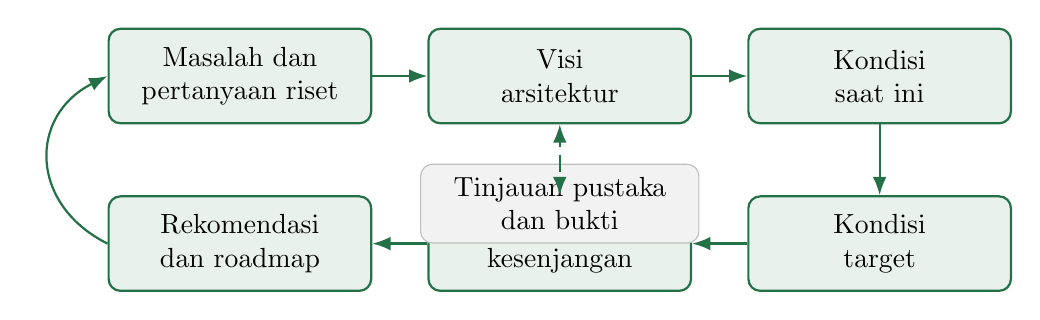
\begin{tikzpicture}[
  admphase/.style={rectangle, rounded corners=1.5mm, draw=praditagreen,
    fill=praditagreen!10, thick, align=center, text width=31mm,
    minimum height=12mm},
  flow/.style={-Latex, thick, draw=praditagreen},
  note/.style={rectangle, rounded corners=1.5mm, draw=gray!50,
    fill=gray!10, align=center, text width=33mm, minimum height=10mm}
]
  \node[admphase] (problem) {Masalah dan\\pertanyaan riset};
  \node[admphase, right=7mm of problem] (vision) {Visi\\arsitektur};
  \node[admphase, right=7mm of vision] (baseline) {Kondisi\\saat ini};
  \node[admphase, below=9mm of baseline] (target) {Kondisi\\target};
  \node[admphase, left=7mm of target] (gap) {Analisis\\kesenjangan};
  \node[admphase, left=7mm of gap] (roadmap) {Rekomendasi\\dan roadmap};

  \draw[flow] (problem) -- (vision);
  \draw[flow] (vision) -- (baseline);
  \draw[flow] (baseline) -- (target);
  \draw[flow] (target) -- (gap);
  \draw[flow] (gap) -- (roadmap);
  \draw[flow] (roadmap.west) .. controls +(-10mm,5mm) and +(-10mm,-5mm) ..
    (problem.west);

  \node[note, below=5mm of vision] (evidence) {Tinjauan pustaka\\dan bukti};
  \draw[flow, dashed] (evidence) -- (vision);
  \draw[flow, dashed] (evidence) -- (gap);
\end{tikzpicture}
}
\caption{Penyederhanaan ADM untuk analisis makalah individual.}
\label{fig:adm-lite-ch3}
\end{figure}

\subsection{Visi Arsitektur}

Visi arsitektur adalah pernyataan awal tentang arah perubahan yang ingin
dicapai. Visi ini tidak perlu panjang, tetapi harus cukup jelas untuk menjawab
tiga hal: masalah apa yang ingin diubah, hasil apa yang diharapkan, dan batas
mana yang tidak akan dibahas. Visi arsitektur juga perlu menyebut pemangku
kepentingan utama karena perubahan arsitektur hampir selalu memengaruhi lebih
dari satu pihak.

Dalam makalah, visi arsitektur membantu pembaca memahami posisi naskah sejak
awal. Jika topik mahasiswa adalah integrasi layanan kesehatan daerah, visi
arsitektur menjelaskan apakah fokusnya pada interoperabilitas data, alur
layanan pasien, tata kelola API, kepatuhan data pribadi, atau kombinasi yang
masih dapat dikelola. Tanpa visi semacam ini, makalah mudah melebar.

\subsection{Tinjauan Pustaka}

Tinjauan pustaka bukan kumpulan ringkasan artikel. Tinjauan pustaka adalah
cara menunjukkan bahwa penulis memahami percakapan akademik dan profesional
yang relevan dengan topiknya. Pustaka dipilih untuk menjawab kebutuhan
argumen: definisi konsep, temuan penelitian, kerangka kerja, praktik baik,
standar, regulasi, dan celah yang masih dapat dikaji.

Untuk bab ini, tinjauan pustaka awal sebaiknya memuat sedikitnya sepuluh
rujukan yang bermakna. Jumlah tersebut bukan angka magis, tetapi batas awal
agar mahasiswa tidak hanya bergantung pada satu atau dua sumber. Pada tahap
berikutnya, daftar ini dapat berkembang sesuai kebutuhan analisis dan target
jurnal atau konferensi.

\subsection{Manajer Referensi dan Bibliografi Kerja}

Manajer referensi membantu mahasiswa menyimpan metadata, mengelompokkan
sumber, menulis catatan ringkas, dan menghasilkan daftar pustaka secara
konsisten. Alat yang digunakan boleh berbeda, tetapi disiplin kerjanya sama:
setiap sumber yang disimpan harus memiliki alasan pemakaian. Bibliografi kerja
tidak cukup berisi judul dan tautan; ia perlu mencatat konsep utama, metode,
konteks, temuan penting, dan hubungan sumber tersebut dengan pertanyaan riset.

\subsection*{Glosarium Mini}

\begin{description}
  \item[ADM] Siklus berpikir dalam TOGAF untuk mengembangkan arsitektur
        enterprise secara bertahap.
  \item[TOGAF-lite] Pemakaian prinsip TOGAF secara selektif dan ringan untuk
        kebutuhan analisis makalah.
  \item[Visi arsitektur] Pernyataan arah perubahan arsitektur yang menjelaskan
        masalah, hasil yang diharapkan, ruang lingkup, dan pemangku
        kepentingan.
  \item[Concern] Kepentingan, kebutuhan, risiko, atau kekhawatiran pemangku
        kepentingan terhadap perubahan arsitektur.
  \item[Bibliografi kerja] Daftar pustaka yang masih berkembang dan disertai
        catatan kegunaan tiap sumber.
  \item[Matriks sintesis] Tabel yang membandingkan beberapa sumber berdasarkan
        konsep, metode, temuan, dan relevansinya dengan makalah.
\end{description}

\section{Kerangka Berpikir}

Bab ini menggunakan alur berpikir yang sederhana: pertanyaan riset menentukan
kebutuhan bukti; kebutuhan bukti mengarahkan pencarian pustaka; pustaka
membantu mempertajam visi arsitektur; visi arsitektur menjadi dasar analisis
kondisi saat ini, target, kesenjangan, dan rekomendasi.

\begin{figure}[htbp]
\centering
\scalebox{0.88}{
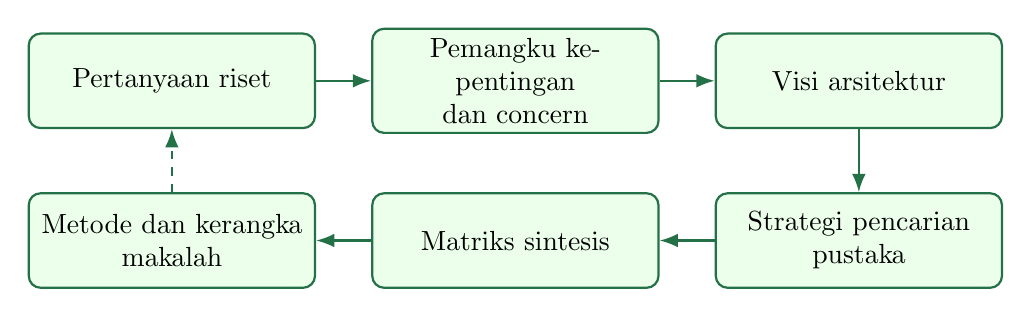
\begin{tikzpicture}[
  box/.style={rectangle, rounded corners=1.5mm, draw=praditagreen,
    fill=green!8, thick, align=center, text width=34mm, minimum height=12mm},
  link/.style={-Latex, thick, draw=praditagreen}
]
  \node[box] (rq) {Pertanyaan riset};
  \node[box, right=7mm of rq] (stake) {Pemangku kepentingan\\dan concern};
  \node[box, right=7mm of stake] (vision) {Visi arsitektur};
  \node[box, below=8mm of vision] (search) {Strategi pencarian\\pustaka};
  \node[box, left=7mm of search] (matrix) {Matriks sintesis};
  \node[box, left=7mm of matrix] (method) {Metode dan kerangka\\makalah};

  \draw[link] (rq) -- (stake);
  \draw[link] (stake) -- (vision);
  \draw[link] (vision) -- (search);
  \draw[link] (search) -- (matrix);
  \draw[link] (matrix) -- (method);
  \draw[link, dashed] (method) -- (rq);
\end{tikzpicture}
}
\caption{Hubungan antara visi arsitektur dan fondasi pustaka.}
\label{fig:vision-literature-loop}
\end{figure}

Kerangka ini sengaja dibuat berulang. Setelah membaca pustaka, mahasiswa
mungkin menyadari bahwa pertanyaan risetnya terlalu lebar. Setelah memetakan
pemangku kepentingan, mahasiswa mungkin melihat bahwa visi awalnya terlalu
teknis dan belum menjawab kebutuhan organisasi. Revisi semacam ini bukan tanda
kegagalan. Justru di situlah penulisan akademik mulai matang.

\section{Konteks Indonesia}

Makalah yang baik tidak hanya mengutip konsep global, tetapi juga memahami
konteks tempat masalah muncul. Untuk kasus Indonesia, konteks tersebut dapat
mencakup regulasi, kebijakan tata kelola data, karakter organisasi, tingkat
kematangan digital, serta ketersediaan sumber rujukan lokal. Misalnya, topik
tata kelola data pribadi perlu membaca kerangka perlindungan data pribadi
\cite{uupdp2022}. Topik sistem elektronik dan transaksi digital perlu
memperhatikan aturan penyelenggaraan sistem elektronik \cite{pp712019}.
Topik pertukaran data pemerintah dapat mengacu pada kerangka Satu Data
Indonesia \cite{satudata}. Topik layanan keuangan digital dapat
mempertimbangkan standar API pembayaran nasional \cite{snapbi}.

Pada saat yang sama, mahasiswa perlu berhati-hati. Dokumen regulasi bukan
pengganti artikel ilmiah. Regulasi memberi batas dan konteks; artikel ilmiah
membantu membangun konsep, metode, dan perbandingan. Keduanya saling
melengkapi. Untuk pencarian literatur, mahasiswa dapat mengombinasikan sumber
internasional, repositori nasional, artikel jurnal Indonesia, prosiding
konferensi, dokumen regulator, dan laporan institusi. Yang penting bukan
banyaknya sumber, melainkan kemampuan menjelaskan mengapa sumber itu dipakai.

\section{Studi Kasus Utama: Visi Arsitektur Bank Wanua}

Kasus Bank Wanua digunakan untuk menunjukkan bagaimana topik awal dapat diubah
menjadi visi arsitektur dan kebutuhan pustaka. Misalkan topik mahasiswa adalah
modernisasi layanan digital bank daerah. Rumusan masalah awalnya berbunyi:
``Layanan digital Bank Wanua sulit berkembang karena data nasabah, proses
persetujuan produk, dan kanal layanan masih tersebar di beberapa sistem
lama.''

Rumusan tersebut sudah berguna, tetapi belum cukup untuk makalah. Mahasiswa
perlu memperjelas arah perubahan. Salah satu visi arsitektur awal dapat
dirumuskan sebagai berikut:

\begin{quote}
Bank Wanua membutuhkan arsitektur layanan digital yang memungkinkan integrasi
data nasabah, orkestrasi proses produk, dan pembukaan API secara terkendali,
sehingga pengembangan layanan baru dapat berlangsung lebih cepat tanpa
mengabaikan keamanan, kepatuhan, dan keberlanjutan sistem lama.
\end{quote}

Visi ini memuat beberapa keputusan awal. Fokusnya bukan mengganti seluruh
sistem inti bank, melainkan mengelola integrasi, proses, dan API. Nilai
bisnisnya adalah percepatan layanan baru. Risikonya adalah keamanan,
kepatuhan, dan keberlanjutan sistem lama. Dari sini, kebutuhan pustaka menjadi
lebih jelas: mahasiswa perlu membaca tentang arsitektur enterprise, platform
digital, tata kelola API, modernisasi sistem lama, dan regulasi sektor
keuangan.

\begin{table}[htbp]
\centering
\scriptsize
\caption{Contoh pemetaan visi arsitektur Bank Wanua.}
\label{tab:bank-wanua-vision}
\begin{tabularx}{\textwidth}{@{}p{0.24\textwidth} X@{}}
\hline
\textbf{Elemen} & \textbf{Rumusan awal} \\
\hline
Masalah utama & Data nasabah, proses produk, dan kanal digital belum
terintegrasi secara memadai. \\
Pemangku kepentingan & Pimpinan bank, unit bisnis, unit kepatuhan, tim
teknologi, mitra layanan digital, dan nasabah. \\
Hasil yang diharapkan & Layanan baru dapat dirancang dan diluncurkan lebih
cepat dengan kendali keamanan dan kepatuhan yang jelas. \\
Ruang lingkup & Integrasi data, orkestrasi proses, tata kelola API, dan
hubungan dengan sistem lama. \\
Batasan & Tidak membahas penggantian penuh core banking dan tidak menyusun
rancangan teknis rinci sampai level kode. \\
Kebutuhan pustaka & EA, platform digital, API, tata kelola data, modernisasi
sistem lama, dan regulasi keuangan digital. \\
\hline
\end{tabularx}
\end{table}

\section{Langkah Analisis dan Artefak Pendukung}

Bagian ini menjadi panduan kerja individual. Setiap langkah sebaiknya
menghasilkan catatan yang dapat dipakai kembali dalam makalah.

\subsection{Langkah 1: Kunci Pertanyaan Riset}

Ambil pertanyaan riset dari Bab~\ref{ch:strategi-bisnis}. Pastikan pertanyaan
tersebut tidak terlalu luas. Pertanyaan seperti ``Bagaimana transformasi
digital memengaruhi perusahaan?'' masih terlalu umum. Pertanyaan yang lebih
siap dianalisis misalnya: ``Bagaimana TOGAF-lite dapat digunakan untuk
merancang integrasi layanan digital pada bank daerah dengan mempertimbangkan
tata kelola API dan kepatuhan data?''

\subsection{Langkah 2: Peta Pemangku Kepentingan dan Concern}

Daftarkan pemangku kepentingan yang terdampak oleh perubahan arsitektur. Untuk
masing-masing pihak, tuliskan kebutuhan atau kekhawatirannya. Jangan hanya
menulis jabatan. Tuliskan kepentingan yang perlu dijawab dalam makalah.
Pimpinan mungkin peduli pada biaya dan manfaat. Unit kepatuhan peduli pada
risiko regulasi. Tim teknologi peduli pada kompleksitas integrasi. Pengguna
peduli pada kenyamanan dan keandalan layanan.

\subsection{Langkah 3: Tetapkan Prinsip Arsitektur}

Prinsip arsitektur adalah aturan berpikir yang membantu memilih solusi.
Contohnya: data penting harus memiliki pemilik yang jelas; API yang dibuka ke
mitra harus memiliki mekanisme pengendalian akses; perubahan sistem lama harus
dilakukan bertahap; dan setiap rekomendasi harus dapat dikaitkan dengan nilai
bisnis. Prinsip tidak perlu banyak. Tiga sampai lima prinsip yang tajam lebih
berguna daripada daftar panjang yang tidak dipakai.

\subsection{Langkah 4: Rumuskan Visi Arsitektur}

Tuliskan visi arsitektur dalam satu paragraf utama. Paragraf itu harus
menjawab masalah, arah perubahan, nilai yang diharapkan, ruang lingkup, dan
batasan. Jika paragraf terasa terlalu panjang, pecah menjadi pernyataan visi
dan daftar batasan. Visi yang baik tidak menjanjikan segalanya; ia memberi
arah yang cukup jelas untuk dianalisis.

\subsection{Langkah 5: Susun Strategi Pencarian Pustaka}

Strategi pencarian pustaka sebaiknya ditulis sebelum mahasiswa mengumpulkan
artikel. Mulailah dari konsep utama dalam pertanyaan riset. Untuk topik Bank
Wanua, kata kunci dapat mencakup \textit{enterprise architecture},
\textit{digital platform}, \textit{API governance},
\textit{legacy system modernization}, \textit{banking digital transformation},
\textit{data governance}, dan \textit{TOGAF}. Padankan kata kunci global
dengan istilah Indonesia bila diperlukan, misalnya ``arsitektur enterprise'',
``tata kelola data'', dan ``layanan keuangan digital''.

\subsection{Langkah 6: Seleksi dan Catat Referensi}

Setiap referensi perlu diseleksi berdasarkan relevansi, mutu, dan fungsi dalam
makalah. Buku kerangka kerja dapat dipakai untuk definisi dan konsep dasar.
Artikel jurnal membantu membangun temuan akademik. Regulasi memberi konteks
batas. Standar profesional memberi bahasa praktik. Catatan referensi minimal
memuat: tujuan sumber, konsep penting, metode atau konteks, temuan utama, dan
alasan sumber tersebut dipakai.

\subsection{Langkah 7: Buat Matriks Sintesis}

Matriks sintesis membantu mahasiswa membandingkan sumber, bukan sekadar
meringkas satu per satu. Gunakan kolom yang sesuai dengan topik. Untuk topik
platform digital, kolom dapat mencakup definisi platform, peran ekosistem,
mekanisme tata kelola, implikasi arsitektur, dan celah riset. Literatur
tentang platform dan ekosistem digital, misalnya, dapat membantu menjelaskan
mengapa arsitektur tidak hanya berbicara tentang aplikasi internal, tetapi
juga hubungan antara organisasi, pengguna, dan mitra
\cite{parker2016platform,cusumano2019business,evans2016matchmakers}.

\subsection{Langkah 8: Tulis Metode Awal}

Metode awal menjelaskan bagaimana makalah akan menggunakan TOGAF-lite.
Contohnya: penelitian konseptual ini menggunakan adaptasi ringan ADM untuk
menyusun visi arsitektur, memetakan kondisi saat ini dan target, melakukan
analisis kesenjangan, serta merumuskan roadmap awal. Tinjauan pustaka
digunakan untuk membangun kerangka konseptual dan memvalidasi kategori
analisis. Metode awal seperti ini belum final, tetapi sudah cukup untuk
mengarahkan penulisan.

\begin{table}[htbp]
\centering
\scriptsize
\caption{Artefak pendukung Bab 3 dan fungsinya dalam makalah.}
\label{tab:artefak-bab3}
\begin{tabularx}{\textwidth}{@{}p{0.25\textwidth} p{0.31\textwidth} X@{}}
\hline
\textbf{Artefak} & \textbf{Isi minimum} & \textbf{Dipakai untuk bagian makalah} \\
\hline
Visi arsitektur & Masalah, arah perubahan, nilai, ruang lingkup, batasan &
Pendahuluan, metode, dan pembahasan awal. \\
Peta stakeholder-concern & Pihak terdampak dan kepentingan utamanya & Latar
belakang, analisis kebutuhan, diskusi risiko. \\
Log pencarian pustaka & Kata kunci, sumber pencarian, kriteria seleksi &
Metode tinjauan pustaka. \\
Bibliografi kerja & Minimal sepuluh rujukan dengan catatan kegunaan &
Tinjauan pustaka dan daftar pustaka. \\
Matriks sintesis & Perbandingan konsep, metode, temuan, dan relevansi &
Kerangka konseptual dan pembahasan. \\
Outline metode & Penjelasan penggunaan TOGAF-lite dan ADM & Bagian metode atau
pendekatan penelitian. \\
\hline
\end{tabularx}
\end{table}

\section{Integrasi ke Makalah Publikasi}

Bab ini berkontribusi langsung pada tiga bagian naskah: tinjauan pustaka,
kerangka konseptual, dan metode. Visi arsitektur biasanya tidak ditempatkan
sebagai artefak mentah yang berdiri sendiri. Ia diterjemahkan menjadi narasi
dalam pendahuluan dan metode. Matriks sintesis tidak selalu perlu dimasukkan
penuh ke naskah, tetapi hasil sintesisnya harus tampak dalam kerangka
konseptual dan pembahasan.

\subsection{Dari Visi ke Pendahuluan}

Pendahuluan makalah dapat menggunakan visi arsitektur untuk menjelaskan
urgensi. Contoh kalimat:

\begin{quote}
Penelitian ini membahas kebutuhan arsitektur layanan digital pada bank daerah
yang menghadapi tekanan untuk mempercepat peluncuran layanan baru, menjaga
kepatuhan data, dan tetap mempertahankan keberlanjutan sistem lama.
\end{quote}

Kalimat tersebut lebih kuat daripada pernyataan umum bahwa ``transformasi
digital sangat penting''. Ia menunjukkan konteks, tekanan perubahan, dan batas
topik.

\subsection{Dari Pustaka ke Kerangka Konseptual}

Tinjauan pustaka perlu diolah menjadi hubungan antar-konsep. Misalnya, konsep
platform digital membantu menjelaskan hubungan antara penyedia layanan,
pengguna, dan mitra \cite{parker2016platform,cusumano2019business}. Konsep
API membantu menjelaskan bagaimana kapabilitas organisasi dapat dibuka dan
dikelola sebagai layanan \cite{jacobson2011apis,medjaoui2018continuous}.
Konsep \textit{operating model} dan arsitektur enterprise membantu menautkan
pilihan teknologi dengan proses dan tata kelola organisasi
\cite{ross2006enterprise,ross2019designed}. Hubungan antar-konsep itulah yang
menjadi kerangka konseptual, bukan sekadar daftar definisi.

\subsection{Dari ADM ke Metode}

Metode makalah dapat menjelaskan bahwa analisis dilakukan melalui adaptasi
ringan ADM. Tahapannya mencakup perumusan visi arsitektur, pemetaan kondisi
saat ini, perumusan kondisi target, analisis kesenjangan, dan penyusunan
roadmap. Karena makalah ini bersifat individual dan akademik, keluaran ADM
dipilih secara selektif. Artefak yang dipakai hanyalah yang memperjelas
argumen penelitian.

\section{Diskusi Kritis, Trade-off, dan Perangkap Umum}

\subsection{Trade-off Pemakaian TOGAF-lite}

TOGAF-lite berguna karena memberi struktur tanpa menuntut dokumentasi yang
terlalu berat. Namun, penyederhanaan memiliki risiko. Jika terlalu
disederhanakan, TOGAF hanya menjadi label. Jika terlalu formal, makalah
berubah menjadi dokumen prosedural yang sulit dibaca. Mahasiswa perlu menjaga
keseimbangan: cukup disiplin untuk menunjukkan tahapan analisis, tetapi cukup
ringkas agar naskah tetap fokus pada argumen.

\begin{table}[htbp]
\centering
\scriptsize
\caption{Trade-off dalam Bab 3.}
\label{tab:tradeoff-bab3}
\begin{tabularx}{\textwidth}{@{}p{0.23\textwidth} X X@{}}
\hline
\textbf{Keputusan} & \textbf{Jika terlalu ringan} & \textbf{Jika terlalu berat} \\
\hline
TOGAF-lite & Menjadi tempelan istilah tanpa metode jelas & Naskah penuh
artefak dan kehilangan argumen utama. \\
Tinjauan pustaka & Sumber sedikit dan klaim lemah & Terlalu banyak kutipan
tanpa sintesis. \\
Visi arsitektur & Arah perubahan kabur & Visi terlalu luas dan tidak selesai
dianalisis. \\
Konteks Indonesia & Makalah terasa generik & Pembahasan regulasi menutupi
fokus arsitektur. \\
Metode & Pembaca tidak tahu cara analisis dilakukan & Metode terlalu teknis
untuk target naskah. \\
\hline
\end{tabularx}
\end{table}

\subsection{Perangkap Umum}

Perangkap pertama adalah memakai TOGAF sebagai daftar fase yang ditempelkan ke
makalah tanpa hubungan yang nyata dengan pertanyaan riset. Hindari menulis
bahwa penelitian ``menggunakan ADM'' tetapi tidak menunjukkan bagaimana setiap
tahap membantu analisis. Perangkap kedua adalah mengumpulkan referensi hanya
karena judulnya mirip. Referensi harus dipilih karena memberi konsep, metode,
temuan, atau konteks yang benar-benar diperlukan.

Perangkap ketiga adalah menulis visi arsitektur terlalu normatif, misalnya
``membangun sistem digital yang aman, cepat, efisien, dan terintegrasi''.
Pernyataan seperti itu terdengar baik, tetapi belum analitis. Apa yang
diintegrasikan? Aman terhadap risiko apa? Cepat untuk proses siapa? Efisien
dibandingkan kondisi apa? Pertanyaan semacam ini perlu dijawab agar visi
menjadi bahan analisis, bukan slogan.

\section{Latihan Terapan Individual}

Latihan pada bab ini dikerjakan secara individual dan menjadi bahan langsung
untuk makalah publikasi.

\subsection*{Latihan 3.1: Visi Arsitektur Satu Halaman}

Tulis visi arsitektur untuk topik makalah masing-masing. Gunakan struktur
berikut:

\begin{enumerate}
  \item judul topik;
  \item masalah utama dalam dua sampai tiga kalimat;
  \item pemangku kepentingan utama dan concern-nya;
  \item pernyataan visi arsitektur;
  \item ruang lingkup dan batasan;
  \item nilai yang diharapkan;
  \item risiko atau asumsi awal.
\end{enumerate}

\subsection*{Latihan 3.2: Strategi Pencarian dan Bibliografi Awal}

Susun strategi pencarian pustaka. Tuliskan kata kunci utama, kombinasi kata
kunci, sumber pencarian, dan kriteria seleksi. Kumpulkan sedikitnya sepuluh
referensi awal. Untuk setiap referensi, tuliskan satu sampai tiga kalimat
tentang kegunaannya bagi makalah.

\subsection*{Latihan 3.3: Matriks Sintesis Lima Referensi Terkuat}

Pilih lima referensi yang paling relevan. Bandingkan kelimanya dalam matriks
yang memuat konsep utama, konteks, metode atau pendekatan, temuan penting, dan
hubungan dengan pertanyaan riset. Setelah itu, tulis satu paragraf sintesis.
Paragraf tersebut harus menunjukkan hubungan antar-sumber, bukan meringkas
sumber secara terpisah.

\subsection*{Latihan 3.4: Paragraf Metode Awal}

Tulis satu paragraf yang menjelaskan bagaimana makalah menggunakan
TOGAF-lite. Paragraf ini minimal memuat alasan memilih TOGAF-lite, tahapan
analisis yang digunakan, artefak yang dihasilkan, dan peran tinjauan pustaka
dalam analisis.

\begin{table}[htbp]
\centering
\scriptsize
\caption{Rubrik latihan Bab 3.}
\label{tab:rubrik-bab3}
\begin{tabularx}{\textwidth}{@{}p{0.25\textwidth} X X@{}}
\hline
\textbf{Komponen} & \textbf{Indikator baik} & \textbf{Perlu diperbaiki bila} \\
\hline
Visi arsitektur & Masalah, arah perubahan, nilai, ruang lingkup, dan batasan
jelas & Masih berupa slogan atau terlalu luas. \\
Stakeholder-concern & Pihak terdampak dan kepentingannya dapat dibedakan &
Hanya berisi daftar jabatan. \\
Bibliografi awal & Minimal sepuluh sumber relevan dan diberi catatan kegunaan
& Sumber dipilih hanya karena mudah ditemukan. \\
Matriks sintesis & Menunjukkan hubungan antar-sumber & Berisi ringkasan
artikel satu per satu. \\
Metode awal & Menjelaskan penggunaan TOGAF-lite secara operasional & Hanya
menyebut TOGAF tanpa tahapan analisis. \\
\hline
\end{tabularx}
\end{table}

\subsection*{Refleksi Singkat}

Jawab tiga pertanyaan berikut dalam catatan pribadi:

\begin{enumerate}
  \item Bagian mana dari visi arsitektur yang masih paling kabur?
  \item Referensi apa yang paling membantu mengubah cara Anda melihat masalah?
  \item Apa yang perlu dipersempit agar makalah dapat selesai sebagai naskah
        publikasi individual?
\end{enumerate}

\section{Ringkasan, Refleksi, dan Jembatan}

\subsection*{Poin Kunci}

\begin{itemize}
  \item TOGAF-lite digunakan sebagai kerangka berpikir ringan, bukan sebagai
        kewajiban membuat seluruh artefak TOGAF.
  \item ADM membantu mahasiswa menata analisis dari masalah menuju visi,
        kondisi saat ini, kondisi target, kesenjangan, dan rekomendasi.
  \item Visi arsitektur memberi arah perubahan yang jelas dan membatasi ruang
        lingkup makalah.
  \item Tinjauan pustaka memberi dasar akademik untuk konsep, metode, dan
        argumen.
  \item Bibliografi kerja dan matriks sintesis adalah jembatan antara aktivitas
        membaca dan penulisan naskah.
\end{itemize}

\subsection*{Menjawab Pertanyaan Pemandu}

Perubahan arsitektur yang dibahas dalam makalah harus dinyatakan sebagai visi
yang spesifik, bukan keinginan umum untuk ``bertransformasi digital''.
Pemangku kepentingan perlu dipetakan karena setiap perubahan arsitektur
membawa dampak yang berbeda bagi pimpinan, unit bisnis, unit kepatuhan, tim
teknologi, mitra, dan pengguna. ADM dapat disederhanakan menjadi alur analisis
yang menjawab masalah, visi, baseline, target, kesenjangan, dan rekomendasi.
Literatur dipilih untuk memperkuat konsep, metode, konteks, dan pembahasan.
Visi arsitektur dan tinjauan pustaka menyatu ketika keduanya digunakan untuk
menulis kerangka konseptual dan metode makalah.

\subsection*{Uji Mandiri}

\begin{enumerate}
  \item Jelaskan perbedaan antara menggunakan TOGAF secara penuh dan
        menggunakan TOGAF-lite untuk makalah individual.
  \item Ambil satu pertanyaan riset Anda. Tuliskan tiga kata kunci global dan
        tiga kata kunci Indonesia yang relevan untuk pencarian pustaka.
  \item Pilih satu referensi terkuat dari bibliografi awal. Jelaskan apakah
        referensi itu dipakai untuk definisi, kerangka konsep, metode,
        konteks, atau pembahasan.
\end{enumerate}

\subsection*{Jembatan ke Bab Berikutnya}

Bab berikutnya masuk ke arsitektur bisnis. Jika Bab 3 menjawab arah perubahan
dan fondasi akademik, Bab 4 mulai membedah proses, kapabilitas, nilai, dan
pemangku kepentingan bisnis secara lebih rinci. Visi arsitektur yang sudah
dibuat pada bab ini akan dipakai untuk memilih kapabilitas mana yang penting,
proses mana yang bermasalah, dan nilai bisnis apa yang harus dijaga dalam
rekomendasi makalah.

\section{Bacaan Lanjutan dan Lampiran}

\subsection*{Bacaan Inti}

\begin{itemize}
  \item The Open Group Architecture Framework versi terbaru sebagai rujukan
        utama TOGAF dan ADM \cite{togaf10}.
  \item Ross, Weill, dan Robertson untuk memahami hubungan antara enterprise
        architecture, operating model, dan fondasi eksekusi
        \cite{ross2006enterprise}.
  \item Ross, Beath, dan Mocker untuk melihat bagaimana organisasi merancang
        ulang dirinya dalam ekonomi digital \cite{ross2019designed}.
\end{itemize}

\subsection*{Bacaan untuk Memperdalam Topik}

\begin{itemize}
  \item Untuk topik platform dan ekosistem digital, baca rujukan tentang
        platform dan pasar dua sisi
        \cite{parker2016platform,cusumano2019business,evans2016matchmakers}.
  \item Untuk topik API dan integrasi layanan, baca rujukan tentang API
        sebagai produk dan tata kelola API
        \cite{jacobson2011apis,medjaoui2018continuous}.
  \item Untuk topik modernisasi sistem dan arsitektur perangkat lunak, baca
        pembahasan tentang monolith dan microservices \cite{newman2021building}.
  \item Untuk konteks Indonesia, sesuaikan rujukan dengan topik: perlindungan
        data pribadi \cite{uupdp2022}, penyelenggaraan sistem elektronik
        \cite{pp712019}, Satu Data Indonesia \cite{satudata}, atau standar API
        pembayaran nasional \cite{snapbi}.
\end{itemize}

\subsection*{Lampiran Kerja Bab 3}

Gunakan templat ringkas berikut sebagai catatan kerja:

\begin{description}
  \item[Topik makalah] Tuliskan topik dalam satu kalimat.
  \item[Pertanyaan riset] Tuliskan pertanyaan riset utama dan, bila perlu,
        satu subpertanyaan.
  \item[Visi arsitektur] Tuliskan arah perubahan dalam satu paragraf.
  \item[Stakeholder-concern] Tuliskan minimal empat pihak dan concern
        masing-masing.
  \item[Kata kunci pustaka] Tuliskan kata kunci utama dalam bahasa Inggris dan
        Indonesia.
  \item[Bibliografi awal] Tuliskan minimal sepuluh referensi beserta catatan
        kegunaan.
  \item[Metode awal] Jelaskan bagaimana TOGAF-lite dipakai dalam analisis.
\end{description}
\setlength{\emergencystretch}{0pt}

    \chapter[Business Architecture dan Tinjauan Pustaka v1]{Business Architecture: Memetakan Kapabilitas, Value Stream, dan Tinjauan Pustaka v1}
\label{ch:business-architecture}
\setlength{\emergencystretch}{2em}

\section*{Tujuan Pembelajaran}
\begin{itemize}
  \item Menjelaskan peran Business Architecture dalam menghubungkan strategi,
        operating model, dan kebutuhan perubahan arsitektur enterprise.
  \item Menyusun peta kapabilitas bisnis yang membedakan kapabilitas inti,
        pendukung, dan tata kelola.
  \item Memetakan value stream untuk menemukan titik masalah, kebutuhan data,
        aplikasi pendukung, dan peluang perbaikan.
  \item Mengubah artefak Business Architecture menjadi narasi analisis domain
        bisnis dan draf tinjauan pustaka v1 untuk makalah publikasi.
\end{itemize}

Tujuan pertama mendukung CLO 1 dan CLO 3. Tujuan kedua sampai keempat
mendukung CLO 3, CLO 6, dan CLO 7 karena mahasiswa diminta menyusun artefak
BDAT sekaligus menjadikannya argumen akademik dalam makalah individual.

\section{Ringkasan Awal Bab}

Bab ini membahas Business Architecture sebagai jembatan antara strategi
organisasi dan rancangan arsitektur yang lebih rinci. Pada Bab~\ref{ch:strategi-bisnis},
mahasiswa telah merumuskan masalah, pertanyaan riset, dan kontribusi awal.
Pada Bab~\ref{ch:togaf-lite}, mahasiswa menyusun visi arsitektur dan
bibliografi awal. Bab ini mengubah keduanya menjadi analisis domain bisnis:
kapabilitas apa yang harus dimiliki organisasi, alur nilai apa yang menjadi
sumber masalah, dan prioritas perubahan apa yang masuk akal.

Dua artefak utama yang digunakan adalah capability map dan value stream.
Capability map menunjukkan kemampuan organisasi yang perlu dipertahankan,
diperbaiki, atau dibangun. Value stream menunjukkan bagaimana nilai mengalir
dari kebutuhan pengguna sampai hasil yang diterima. Bagi pembaca non-TI,
kedua artefak ini penting karena membantu membahas arsitektur tanpa langsung
tenggelam dalam aplikasi, database, atau infrastruktur.

Keluaran bab ini adalah peta kapabilitas, value stream, prioritas kapabilitas,
dan draf Literature Review v1. Semua keluaran tersebut dipakai untuk
memperkuat bagian tinjauan pustaka, konteks studi kasus, dan analisis domain
bisnis dalam makalah publikasi individual.

\section{Pendahuluan}

Business Architecture menjawab pertanyaan yang tampak sederhana tetapi sering
terabaikan: kemampuan bisnis apa yang harus dimiliki organisasi agar strategi
digitalnya dapat berjalan? Pertanyaan ini berbeda dari pertanyaan tentang
aplikasi apa yang perlu dibangun. Aplikasi adalah salah satu pendukung.
Kemampuan bisnis mencakup proses, peran, aturan keputusan, data yang
dibutuhkan, mitra yang terlibat, ukuran keberhasilan, dan kendali risiko.

Dalam Enterprise Architecture, Business Architecture menjadi pintu masuk
untuk domain lain. Data Architecture membutuhkan kejelasan tentang informasi
apa yang diperlukan bisnis. Application Architecture membutuhkan pemahaman
tentang proses dan kapabilitas mana yang perlu didukung. Technology
Architecture membutuhkan konteks prioritas, risiko, dan skala layanan.
Karena itu, membahas data, aplikasi, dan teknologi sebelum memahami domain
bisnis sering menghasilkan rancangan yang tampak canggih tetapi tidak menjawab
masalah organisasi.

Untuk makalah publikasi, Business Architecture membantu mahasiswa membuat
analisis yang lebih meyakinkan. Penulis dapat menunjukkan bahwa masalah yang
dibahas tidak berdiri sendiri, melainkan muncul dari ketidakselarasan antara
strategi, kapabilitas, value stream, dan tata kelola. Rujukan tentang
Enterprise Architecture sebagai fondasi pelaksanaan strategi menekankan bahwa
arsitektur harus menata hubungan antara model operasi, proses, data, dan
keputusan bisnis \cite{ross2006enterprise}. Pandangan tentang organisasi
digital juga menekankan pentingnya kapabilitas yang dirancang sadar, bukan
hanya proyek teknologi yang berjalan terpisah \cite{ross2019designed}.

\section{Skenario Pembuka dan Pertanyaan Pemandu}

Bank Wanua telah memiliki visi arsitektur awal: memperkuat layanan digital
dengan integrasi data nasabah, orkestrasi proses produk, dan API yang
terkendali. Namun, begitu visi itu dibahas bersama unit bisnis, muncul
pertanyaan yang lebih praktis. Kapabilitas apa yang sebenarnya lemah? Apakah
masalah utama ada pada pemasaran digital, verifikasi nasabah, manajemen
produk, kepatuhan data, layanan mitra, atau analitik nasabah? Jika semua
dinyatakan penting, tidak ada prioritas yang dapat dipertanggungjawabkan.

Direktur bisnis meminta peta sederhana: kemampuan apa yang sudah cukup baik,
kemampuan apa yang perlu diperbaiki, dan kemampuan apa yang harus dibangun
agar Bank Wanua dapat menjadi mitra digital UMKM lokal. Unit kepatuhan
menambahkan pertanyaan lain: pada alur layanan mana data pribadi paling banyak
berpindah tangan? Tim teknologi juga meminta kejelasan: proses mana yang
sebenarnya perlu didukung aplikasi baru, dan proses mana yang dapat diperbaiki
dengan perubahan prosedur atau tata kelola?

Di titik ini, diskusi tidak dapat lagi berhenti pada slogan strategi. Bank
Wanua membutuhkan Business Architecture yang dapat dibaca bersama oleh
pimpinan, unit bisnis, kepatuhan, dan tim teknologi. Mahasiswa yang menulis
makalah tentang kasus ini juga membutuhkan hal yang sama: artefak yang
mengubah masalah organisasi menjadi analisis yang runtut.

\subsection*{Pertanyaan Pemandu}

\begin{enumerate}
  \item Kapabilitas bisnis apa yang paling menentukan keberhasilan visi
        arsitektur?
  \item Bagaimana capability map membantu membedakan masalah inti dari gejala?
  \item Value stream mana yang paling relevan dengan pertanyaan riset?
  \item Bukti apa yang diperlukan agar analisis domain bisnis tidak sekadar
        berdasarkan dugaan?
  \item Bagaimana hasil Business Architecture masuk ke tinjauan pustaka dan
        analisis makalah publikasi?
\end{enumerate}

\section{Mengapa Bab Ini Penting bagi Pembaca Non-TI}

Pembaca non-TI tidak harus menjadi perancang sistem teknis untuk dapat
berkontribusi pada arsitektur enterprise. Justru, banyak keputusan penting
berada di wilayah bisnis: siapa pengguna prioritas, nilai apa yang dijanjikan,
proses apa yang harus distandardisasi, data apa yang harus dipercaya,
pengendalian risiko seperti apa yang wajib ada, dan kapabilitas mana yang
layak didanai terlebih dahulu.

Business Architecture memberi bahasa bersama untuk diskusi tersebut. Dengan
capability map, mahasiswa dapat membicarakan kemampuan organisasi tanpa
terjebak pada nama aplikasi. Dengan value stream, mahasiswa dapat menjelaskan
di bagian mana nilai tersendat, risiko muncul, atau pengalaman pengguna
menurun. Dengan dua artefak ini, rekomendasi dalam makalah menjadi lebih
mudah dipertanggungjawabkan karena pembaca dapat melihat hubungan antara
masalah, bukti, prioritas, dan implikasi.

\section{Konsep Inti dan Glosarium Mini}

\subsection{Business Architecture}

Business Architecture adalah deskripsi terstruktur tentang bagaimana organisasi
menciptakan nilai melalui kapabilitas, proses, informasi, peran, kebijakan,
dan hubungan dengan pemangku kepentingan. Dalam TOGAF, Business Architecture
menjadi salah satu domain utama yang membantu menerjemahkan visi arsitektur ke
dalam struktur bisnis yang dapat dianalisis \cite{togaf10}.

Secara manajerial, Business Architecture dapat dibayangkan sebagai peta
kemampuan organisasi. Peta ini tidak menggambarkan struktur jabatan, tetapi
menggambarkan apa yang harus mampu dilakukan organisasi. Dua unit dapat
berbeda dalam struktur organisasi, tetapi membutuhkan kapabilitas yang sama.
Sebaliknya, satu unit dapat memegang beberapa kapabilitas sekaligus. Karena
itu, capability map biasanya lebih stabil daripada bagan organisasi.

\subsection{Business Capability}

Business capability adalah kemampuan yang dibutuhkan organisasi untuk
menciptakan nilai atau menjalankan mandatnya. Contoh kapabilitas pada bank
daerah adalah akuisisi nasabah UMKM, penilaian kelayakan kredit, manajemen
risiko, pengelolaan data nasabah, layanan kanal digital, pengelolaan mitra,
dan kepatuhan regulasi.

Kapabilitas tidak sama dengan proses. Proses menjelaskan urutan aktivitas.
Kapabilitas menjelaskan kemampuan yang harus ada agar aktivitas dapat berjalan
dengan baik. Satu kapabilitas dapat muncul dalam beberapa proses, dan satu
proses dapat memerlukan beberapa kapabilitas. Perbedaan ini penting karena
makalah arsitektur tidak cukup hanya menggambar alur kerja; ia perlu
menjelaskan kemampuan organisasi yang perlu berubah.

\subsection{Capability Map}

Capability map adalah visualisasi kapabilitas organisasi. Peta ini biasanya
dikelompokkan ke dalam lapisan seperti kapabilitas strategis, kapabilitas inti
pelayanan, dan kapabilitas pendukung. Untuk makalah individual, capability map
tidak harus lengkap seperti dokumen konsultan. Yang lebih penting adalah peta
itu relevan dengan pertanyaan riset dan cukup jelas untuk menjelaskan prioritas
analisis.

\begin{figure}[htbp]
\centering
\scalebox{0.86}{
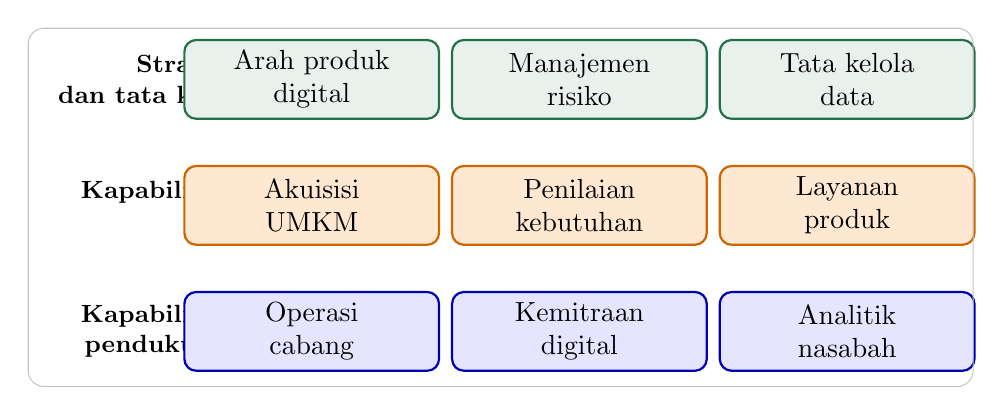
\begin{tikzpicture}[
  capnode/.style={rectangle, rounded corners=1.5mm, draw=praditagreen,
    fill=praditagreen!10, thick, align=center, text width=30mm,
    minimum height=10mm},
  core/.style={rectangle, rounded corners=1.5mm, draw=orange!80!black,
    fill=orange!18, thick, align=center, text width=30mm,
    minimum height=10mm},
  support/.style={rectangle, rounded corners=1.5mm, draw=blue!70!black,
    fill=blue!10, thick, align=center, text width=30mm,
    minimum height=10mm},
  layer/.style={font=\small\bfseries, align=right}
]
  \node[layer] at (-1.0,2.6) {Strategis\\dan tata kelola};
  \node[capnode] (s1) at (1.0,2.6) {Arah produk\\digital};
  \node[capnode] (s2) at (4.4,2.6) {Manajemen\\risiko};
  \node[capnode] (s3) at (7.8,2.6) {Tata kelola\\data};

  \node[layer] at (-1.0,1.0) {Kapabilitas\\inti};
  \node[core] (c1) at (1.0,1.0) {Akuisisi\\UMKM};
  \node[core] (c2) at (4.4,1.0) {Penilaian\\kebutuhan};
  \node[core] (c3) at (7.8,1.0) {Layanan\\produk};

  \node[layer] at (-1.0,-0.6) {Kapabilitas\\pendukung};
  \node[support] (p1) at (1.0,-0.6) {Operasi\\cabang};
  \node[support] (p2) at (4.4,-0.6) {Kemitraan\\digital};
  \node[support] (p3) at (7.8,-0.6) {Analitik\\nasabah};

  \draw[gray!45, rounded corners=2mm] (-2.6,-1.3) rectangle (9.4,3.25);
\end{tikzpicture}
}
\caption{Contoh sederhana capability map untuk layanan digital Bank Wanua.}
\label{fig:capability-map-bank-wanua}
\end{figure}

\subsection{Value Stream}

Value stream adalah alur penciptaan nilai dari kebutuhan awal sampai hasil
yang diterima pengguna atau pemangku kepentingan. Jika capability map
menunjukkan kemampuan yang dibutuhkan, value stream menunjukkan bagaimana
kemampuan itu bekerja bersama dalam satu perjalanan nilai.

Pada Bank Wanua, value stream untuk layanan UMKM dapat dimulai dari menarik
minat calon nasabah, memahami kebutuhan, dan menilai kelayakan. Tahap
berikutnya adalah menawarkan produk, melakukan persetujuan, mengaktifkan
layanan, lalu memantau dan mendukung nasabah. Di setiap tahap, penulis dapat
menanyakan: siapa aktornya, data apa yang digunakan, sistem apa yang
mendukung, risiko apa yang muncul, dan metrik apa yang menunjukkan
keberhasilan.

\subsection{Operating Model dalam Business Architecture}

Operating model menjelaskan tingkat integrasi data dan standardisasi proses
yang dibutuhkan organisasi untuk menjalankan strategi \cite{ross2006enterprise}.
Bab~\ref{ch:strategi-bisnis} telah memperkenalkan konsep ini sebagai alat
membaca strategi. Dalam Bab 4, operating model dipakai lebih operasional:
untuk menilai apakah kapabilitas tertentu perlu distandardisasi, diintegrasikan,
atau dibiarkan berbeda sesuai konteks unit.

Bank Wanua, misalnya, mungkin perlu data nasabah UMKM yang terintegrasi lintas
cabang, tetapi proses pendampingan UMKM boleh tetap menyesuaikan karakter
wilayah. Keputusan semacam ini adalah keputusan Business Architecture. Ia
menentukan apa yang harus seragam, apa yang boleh lokal, dan apa yang harus
terhubung melalui tata kelola data atau API.

\subsection*{Glosarium Mini}

\begin{description}
  \item[Business Architecture] Deskripsi terstruktur tentang kapabilitas,
        proses, informasi, peran, dan kebijakan yang memungkinkan organisasi
        menciptakan nilai.
  \item[Business capability] Kemampuan organisasi untuk menjalankan fungsi
        tertentu, misalnya akuisisi nasabah, manajemen risiko, atau tata
        kelola data.
  \item[Capability map] Peta kapabilitas yang menunjukkan kemampuan inti,
        pendukung, dan tata kelola yang relevan dengan strategi.
  \item[Value stream] Alur penciptaan nilai dari kebutuhan pemangku kepentingan
        sampai hasil yang diterima.
  \item[Pain point] Titik dalam alur nilai yang menimbulkan kelambatan, risiko,
        biaya, duplikasi, atau pengalaman buruk.
  \item[Prioritas kapabilitas] Keputusan tentang kapabilitas mana yang perlu
        dipertahankan, diperbaiki, atau dibangun terlebih dahulu.
\end{description}

\section{Kerangka Berpikir}

Kerangka Bab 4 bergerak dari visi arsitektur menuju analisis domain bisnis.
Pertanyaan riset dan visi arsitektur memberi arah. Capability map menunjukkan
kemampuan yang dibutuhkan. Value stream membantu menemukan titik masalah.
Analisis prioritas menentukan kapabilitas mana yang paling penting. Hasilnya
menjadi bahan analisis domain bisnis dan draf tinjauan pustaka v1.

\begin{figure}[htbp]
\centering
\scalebox{0.86}{
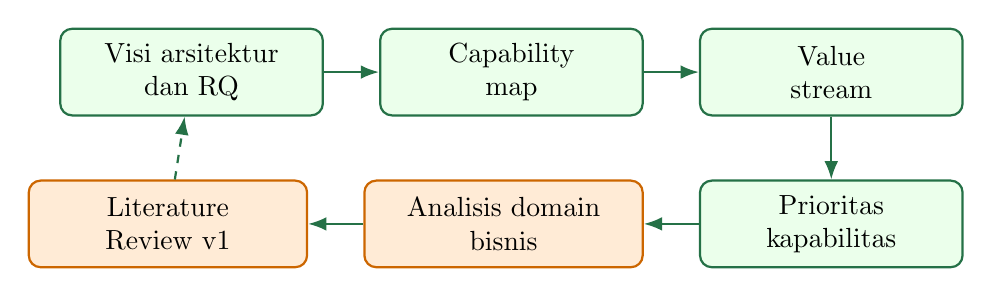
\begin{tikzpicture}[
  box/.style={rectangle, rounded corners=1.5mm, draw=praditagreen,
    fill=green!8, thick, align=center, text width=31mm, minimum height=11mm},
  outnode/.style={rectangle, rounded corners=1.5mm, draw=orange!80!black,
    fill=orange!16, thick, align=center, text width=33mm, minimum height=11mm},
  link/.style={-Latex, thick, draw=praditagreen}
]
  \node[box] (vision) {Visi arsitektur\\dan RQ};
  \node[box, right=7mm of vision] (cap) {Capability\\map};
  \node[box, right=7mm of cap] (stream) {Value\\stream};
  \node[box, below=8mm of stream] (priority) {Prioritas\\kapabilitas};
  \node[outnode, left=7mm of priority] (analysis) {Analisis domain\\bisnis};
  \node[outnode, left=7mm of analysis] (lit) {Literature\\Review v1};

  \draw[link] (vision) -- (cap);
  \draw[link] (cap) -- (stream);
  \draw[link] (stream) -- (priority);
  \draw[link] (priority) -- (analysis);
  \draw[link] (analysis) -- (lit);
  \draw[link, dashed] (lit) -- (vision);
\end{tikzpicture}
}
\caption{Alur berpikir Business Architecture untuk makalah publikasi.}
\label{fig:business-architecture-flow}
\end{figure}

Alur ini tidak harus selalu linear. Saat menyusun capability map, mahasiswa
dapat menemukan bahwa pertanyaan risetnya terlalu teknis. Saat menggambar
value stream, mahasiswa dapat menyadari bahwa masalah utama bukan aplikasi,
melainkan aturan keputusan yang tidak jelas. Saat menulis Literature Review
v1, mahasiswa dapat menemukan konsep yang membuat prioritas kapabilitas perlu
diubah. Revisi semacam ini adalah bagian wajar dari penulisan akademik.

\section{Konteks Indonesia}

Business Architecture di Indonesia perlu memperhatikan variasi kematangan
organisasi. Banyak organisasi memiliki strategi digital yang ambisius, tetapi
kapabilitas bisnisnya belum merata. Cabang atau unit daerah dapat memiliki
cara kerja berbeda. Data pelanggan atau warga sering tersimpan di beberapa
sistem. Proses persetujuan masih bergantung pada dokumen manual. Peran vendor
besar, sementara kemampuan internal untuk mengelola perubahan belum selalu
kuat.

Regulasi juga memengaruhi prioritas kapabilitas. Organisasi yang mengelola
data pribadi perlu memiliki kapabilitas pengelolaan persetujuan, pembatasan
akses, pencatatan penggunaan data, dan penanganan insiden yang sejalan dengan
perlindungan data pribadi \cite{uupdp2022}. Penyelenggara sistem elektronik
perlu memperhatikan kewajiban pengelolaan sistem dan data elektronik
\cite{pp712019}. Organisasi sektor publik yang bertukar data perlu memahami
prinsip Satu Data Indonesia \cite{satudata}. Lembaga keuangan yang membuka
integrasi pembayaran atau kemitraan digital perlu memperhatikan standar Open
API pembayaran nasional \cite{snapbi}.

Konteks lokal juga memengaruhi value stream. Di banyak sektor, pengalaman
pengguna tidak hanya terjadi di kanal digital. Nasabah bank daerah, pasien
rumah sakit, petani, mahasiswa, atau pelaku UMKM masih berinteraksi melalui
kantor cabang, petugas lapangan, agen, WhatsApp, dan dokumen fisik. Karena
itu, Business Architecture yang baik tidak memaksakan narasi serba aplikasi.
Ia membaca alur nilai secara utuh: digital, fisik, manusia, mitra, dan aturan.

\section{Studi Kasus Utama: Business Architecture Bank Wanua}

Visi Bank Wanua adalah menjadi mitra keuangan digital bagi UMKM lokal. Agar
visi tersebut tidak berhenti sebagai slogan, mahasiswa perlu memetakan
kapabilitas yang membuat visi itu mungkin. Peta awal dapat disusun dari tiga
pertanyaan:

\begin{enumerate}
  \item Kapabilitas apa yang langsung berhubungan dengan nilai bagi UMKM?
  \item Kapabilitas apa yang menjaga risiko, kepatuhan, dan keberlanjutan?
  \item Kapabilitas apa yang mendukung integrasi digital dan pembelajaran
        organisasi?
\end{enumerate}

\subsection{Capability Map Bank Wanua}

\begin{table}[htbp]
\centering
\scriptsize
\caption{Capability map awal Bank Wanua untuk layanan digital UMKM.}
\label{tab:capability-bank-wanua}
\begin{tabularx}{\textwidth}{@{}p{0.22\textwidth} p{0.28\textwidth} X X@{}}
\hline
\textbf{Kelompok} & \textbf{Kapabilitas} & \textbf{Kondisi awal} & \textbf{Prioritas} \\
\hline
Strategis dan tata kelola & Perencanaan produk digital & Produk dirancang per
inisiatif, belum memakai portofolio layanan yang jelas & Diperbaiki \\
Strategis dan tata kelola & Manajemen risiko dan kepatuhan & Kontrol kuat,
tetapi sering masuk terlambat dalam rancangan layanan & Diperbaiki \\
Strategis dan tata kelola & Tata kelola data nasabah & Definisi data dan
kepemilikan belum konsisten lintas kanal & Dibangun \\
Kapabilitas inti & Akuisisi nasabah UMKM & Masih bergantung pada cabang dan
relasi lokal & Dipertahankan dan diperkuat \\
Kapabilitas inti & Penilaian kebutuhan dan kelayakan & Data tersebar; asesmen
sering berulang & Diperbaiki \\
Kapabilitas inti & Layanan produk dan transaksi & Kanal digital tersedia,
tetapi integrasi proses belum mulus & Diperbaiki \\
Kapabilitas pendukung & Kemitraan digital & Peluang mitra ada, tetapi aturan
integrasi belum matang & Dibangun \\
Kapabilitas pendukung & Analitik nasabah & Laporan tersedia, tetapi belum
menjadi dasar personalisasi layanan & Dibangun \\
\hline
\end{tabularx}
\end{table}

Tabel~\ref{tab:capability-bank-wanua} tidak dimaksudkan sebagai daftar final.
Ia adalah peta kerja awal. Dalam makalah, mahasiswa perlu menjelaskan dari
mana penilaian kondisi awal diperoleh: dokumen publik, wawancara, observasi,
laporan tahunan, studi literatur, atau asumsi yang dinyatakan secara eksplisit
bila kasus bersifat hipotetis-realistis.

\subsection{Value Stream Layanan UMKM}

Setelah kapabilitas dipetakan, mahasiswa perlu melihat bagaimana kapabilitas
tersebut bekerja dalam alur nilai. Untuk Bank Wanua, salah satu value stream
yang relevan adalah ``UMKM memperoleh layanan pembiayaan dan pembayaran
digital''. Alur ini tidak hanya mencakup aplikasi mobile, tetapi juga
interaksi cabang, verifikasi dokumen, penilaian risiko, aktivasi layanan, dan
pendampingan.

\begin{figure}[htbp]
\centering
\scalebox{0.78}{
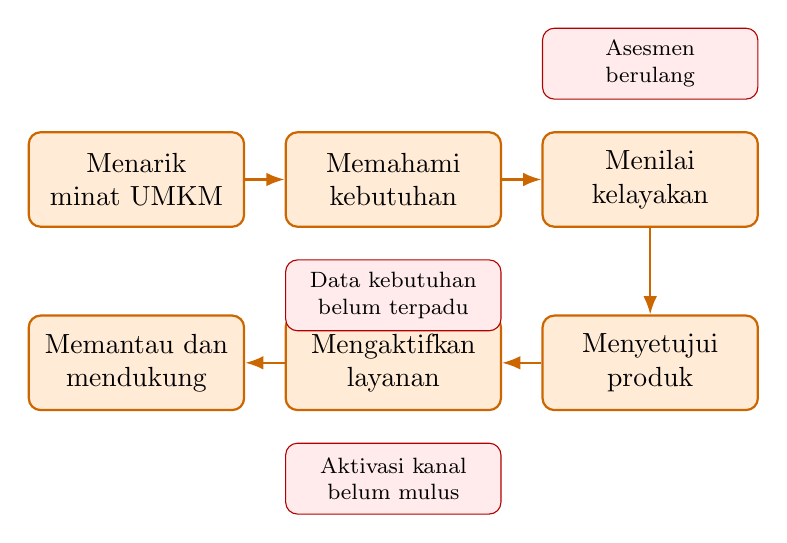
\begin{tikzpicture}[
  stage/.style={rectangle, rounded corners=1.5mm, draw=orange!80!black,
    fill=orange!16, thick, align=center, text width=25mm, minimum height=12mm},
  pain/.style={rectangle, rounded corners=1.5mm, draw=red!70!black,
    fill=red!8, align=center, text width=25mm, minimum height=9mm,
    font=\footnotesize},
  link/.style={-Latex, thick, draw=orange!80!black}
]
  \node[stage] (s1) {Menarik\\minat UMKM};
  \node[stage, right=5mm of s1] (s2) {Memahami\\kebutuhan};
  \node[stage, right=5mm of s2] (s3) {Menilai\\kelayakan};
  \node[stage, below=11mm of s3] (s4) {Menyetujui\\produk};
  \node[stage, left=5mm of s4] (s5) {Mengaktifkan\\layanan};
  \node[stage, left=5mm of s5] (s6) {Memantau dan\\mendukung};

  \draw[link] (s1) -- (s2);
  \draw[link] (s2) -- (s3);
  \draw[link] (s3) -- (s4);
  \draw[link] (s4) -- (s5);
  \draw[link] (s5) -- (s6);

  \node[pain, below=4mm of s2] {Data kebutuhan\\belum terpadu};
  \node[pain, above=4mm of s3] {Asesmen\\berulang};
  \node[pain, below=4mm of s5] {Aktivasi kanal\\belum mulus};
\end{tikzpicture}
}
\caption{Value stream awal layanan UMKM Bank Wanua.}
\label{fig:value-stream-bank-wanua}
\end{figure}

Gambar~\ref{fig:value-stream-bank-wanua} membantu mahasiswa menemukan hubungan
antara kapabilitas dan titik masalah. Jika data kebutuhan UMKM belum terpadu,
kapabilitas tata kelola data dan analitik nasabah perlu diperkuat. Jika
asesmen berulang, kapabilitas penilaian kelayakan dan orkestrasi proses perlu
diperbaiki. Jika aktivasi kanal belum mulus, kapabilitas layanan produk,
integrasi aplikasi, dan tata kelola API mulai terlihat sebagai kebutuhan bab
berikutnya.

\section{Langkah Analisis dan Artefak Pendukung}

Bagian ini menjadi panduan kerja individual untuk menghasilkan artefak Bab 4.
Gunakan organisasi studi kasus yang sama dengan bab sebelumnya.

\subsection{Langkah 1: Tetapkan Ruang Lingkup Domain Bisnis}

Mulailah dari pertanyaan riset dan visi arsitektur. Tentukan layanan, produk,
unit, atau proses yang akan dianalisis. Jangan mencoba memetakan seluruh
organisasi jika makalah hanya membahas satu masalah. Ruang lingkup yang baik
cukup sempit untuk dianalisis, tetapi cukup penting untuk menjawab RQ.

\subsection{Langkah 2: Daftarkan Kapabilitas Bisnis}

Tuliskan kapabilitas yang dibutuhkan agar strategi berjalan. Gunakan kata
benda abstrak yang menunjukkan kemampuan, bukan aktivitas terlalu rinci.
Misalnya, tulis ``manajemen risiko kredit UMKM'', bukan ``mengisi formulir
penilaian''. Tulis ``tata kelola data pelanggan'', bukan ``mengunduh file
Excel''. Kapabilitas yang baik membantu pembaca melihat kemampuan organisasi
yang perlu ditata.

\subsection{Langkah 3: Kelompokkan Kapabilitas}

Kelompokkan kapabilitas ke dalam tiga sampai empat kategori. Kategori umum
adalah strategis dan tata kelola, kapabilitas inti, kapabilitas pendukung, dan
kapabilitas pembelajaran organisasi. Pengelompokan ini membantu pembaca non-TI
memahami mana kemampuan yang langsung menciptakan nilai dan mana yang menjaga
agar nilai itu dapat diberikan secara aman dan berulang.

\subsection{Langkah 4: Nilai Kondisi Awal dan Prioritas}

Untuk setiap kapabilitas, beri penilaian kondisi awal. Gunakan kategori
sederhana: kuat, cukup, lemah, atau belum ada. Setelah itu, tuliskan prioritas:
dipertahankan, diperbaiki, atau dibangun. Hindari memberi semua kapabilitas
prioritas tinggi. Prioritas yang baik harus berani memilih.

\subsection{Langkah 5: Pilih Value Stream Utama}

Pilih satu value stream yang paling relevan dengan RQ. Value stream dapat
berupa perjalanan pengguna, alur layanan, alur persetujuan, atau alur
penciptaan nilai. Tuliskan tahap utama dari awal sampai akhir. Pada setiap
tahap, catat aktor, data, aplikasi, risiko, dan pain point.

\subsection{Langkah 6: Hubungkan Value Stream dengan Kapabilitas}

Tanyakan kapabilitas mana yang mendukung setiap tahap value stream. Hubungan
ini penting karena menunjukkan mengapa sebuah kapabilitas perlu diprioritaskan.
Jika satu kapabilitas muncul di banyak titik masalah, kapabilitas itu mungkin
lebih penting daripada yang awalnya terlihat.

\subsection{Langkah 7: Susun Bukti dan Literatur Pendukung}

Business Architecture tidak boleh hanya berdasarkan intuisi. Catat sumber
bukti untuk setiap klaim. Bukti dapat berupa dokumen organisasi, laporan
tahunan, wawancara, observasi, regulasi, standar, atau literatur akademik.
Gunakan literatur untuk menjelaskan konsep seperti Enterprise Architecture,
operating model, kapabilitas digital, platform, dan tata kelola.

\subsection{Langkah 8: Tulis Narasi Analisis Domain Bisnis}

Ubah capability map dan value stream menjadi narasi. Narasi minimal menjawab:
kapabilitas apa yang paling bermasalah, bagaimana masalah itu terlihat dalam
alur nilai, mengapa masalah itu penting bagi strategi, dan apa implikasinya
untuk domain data, aplikasi, teknologi, API, dan platform pada bab berikutnya.

\begin{table}[htbp]
\centering
\scriptsize
\caption{Artefak Bab 4 dan pemakaiannya dalam makalah.}
\label{tab:artefak-bab4}
\begin{tabularx}{\textwidth}{@{}p{0.24\textwidth} p{0.32\textwidth} X@{}}
\hline
\textbf{Artefak} & \textbf{Isi minimum} & \textbf{Dipakai untuk bagian makalah} \\
\hline
Capability map & Kelompok kapabilitas, kondisi awal, prioritas & Konteks
studi kasus dan analisis domain bisnis. \\
Value stream & Tahap alur nilai, aktor, data, pain point, risiko & Analisis
baseline dan pembahasan masalah. \\
Tabel prioritas kapabilitas & Kapabilitas, alasan prioritas, bukti, dampak &
Gap analysis dan implikasi manajerial. \\
Matriks pustaka bisnis & Konsep, sumber, fungsi dalam argumen, hubungan ke RQ
& Literature Review v1. \\
Narasi analisis bisnis & Dua sampai empat paragraf akademik & Bagian
analysis/results atau studi kasus. \\
\hline
\end{tabularx}
\end{table}

\section{Integrasi ke Makalah Publikasi}

Bab ini memperkuat dua bagian utama makalah: tinjauan pustaka dan analisis
domain bisnis. Pada tinjauan pustaka, mahasiswa menjelaskan konsep Enterprise
Architecture, Business Architecture, operating model, kapabilitas digital, dan
value stream. Pada analisis domain bisnis, mahasiswa menunjukkan bagaimana
konsep tersebut dipakai untuk membaca kasus.

\subsection{Dari Artefak ke Tinjauan Pustaka}

Literature Review v1 tidak perlu langsung sempurna. Pada tahap ini, tujuannya
adalah membuat sintesis awal yang terhubung dengan artefak. Misalnya, jika
capability map menunjukkan lemahnya tata kelola data dan analitik nasabah,
tinjauan pustaka perlu memuat konsep tentang operating model, kapabilitas
digital, dan arsitektur enterprise sebagai fondasi eksekusi strategi
\cite{ross2006enterprise,ross2019designed}. Jika value stream menunjukkan
kebutuhan kemitraan dan layanan API, tinjauan pustaka mulai dapat menyinggung
literatur API dan platform sebagai pengantar untuk bab berikutnya
\cite{jacobson2011apis,parker2016platform}.

\subsection{Struktur Literature Review v1}

Untuk Bab 4, Literature Review v1 dapat disusun dengan pola berikut:

\begin{enumerate}
  \item paragraf tentang Enterprise Architecture sebagai penghubung strategi
        dan eksekusi;
  \item paragraf tentang Business Architecture, capability map, dan value
        stream;
  \item paragraf tentang konteks digital organisasi, misalnya platform, API,
        atau tata kelola data sesuai topik;
  \item paragraf sintesis yang menjelaskan celah atau kebutuhan analisis pada
        studi kasus mahasiswa.
\end{enumerate}

Contoh paragraf sintesis:

\begin{quote}
Literatur Enterprise Architecture menekankan bahwa strategi digital perlu
diterjemahkan ke dalam kapabilitas, proses, dan model operasi yang konsisten.
Dalam kasus bank daerah, kebutuhan integrasi layanan UMKM tidak cukup dibaca
sebagai masalah aplikasi, tetapi sebagai ketidakselarasan antara kapabilitas
akuisisi nasabah, penilaian kelayakan, tata kelola data, dan kemitraan digital.
Oleh karena itu, penelitian ini menggunakan capability map dan value stream
untuk mengidentifikasi kapabilitas prioritas sebelum merumuskan rancangan
arsitektur data, aplikasi, dan teknologi.
\end{quote}

\subsection{Dari Business Architecture ke Analisis}

Dalam bagian analisis, capability map dapat ditempatkan sebagai gambar atau
tabel. Value stream dapat digunakan untuk menjelaskan alur masalah. Yang
penting, artefak tidak berdiri sendiri. Setelah gambar atau tabel, selalu ada
paragraf yang menjelaskan temuan: kapabilitas mana yang lemah, pain point apa
yang muncul, dampaknya pada strategi, dan implikasinya bagi rancangan BDAT.

\section{Diskusi Kritis, Trade-off, dan Perangkap Umum}

\subsection{Trade-off dalam Business Architecture}

Business Architecture memaksa penulis memilih tingkat abstraksi. Jika terlalu
tinggi, capability map menjadi daftar kata besar yang sulit dipakai. Jika
terlalu rinci, peta berubah menjadi prosedur operasional dan kehilangan
fungsi strategis. Value stream juga memiliki trade-off serupa. Jika terlalu
pendek, pain point tidak terlihat. Jika terlalu panjang, pembaca kehilangan
alur utama.

\begin{table}[htbp]
\centering
\scriptsize
\caption{Trade-off utama dalam Business Architecture.}
\label{tab:tradeoff-bab4}
\begin{tabularx}{\textwidth}{@{}p{0.23\textwidth} X X X@{}}
\hline
\textbf{Keputusan} & \textbf{Alternatif} & \textbf{Manfaat} & \textbf{Risiko} \\
\hline
Cakupan capability map & Seluruh organisasi atau satu domain prioritas &
Cakupan luas memberi konteks; cakupan sempit lebih tajam & Terlalu luas
membuat makalah melebar. \\
Level detail kapabilitas & Kapabilitas besar atau subkapabilitas & Detail
membantu prioritas & Terlalu rinci membuat peta sulit dibaca. \\
Value stream & Alur end-to-end atau satu potongan kritis & End-to-end
menunjukkan konteks utuh & Terlalu panjang menyulitkan analisis. \\
Sumber bukti & Data internal, dokumen publik, atau asumsi eksplisit & Bukti
kuat memperkuat klaim & Data sensitif perlu izin dan anonimisasi. \\
Literature Review v1 & Ringkas terarah atau luas eksploratif & Ringkas lebih
mudah disintesis & Terlalu sempit dapat melewatkan konsep penting. \\
\hline
\end{tabularx}
\end{table}

\subsection{Perangkap Umum}

Perangkap pertama adalah menggambar capability map seperti bagan organisasi.
Kapabilitas bukan unit kerja. ``Divisi pemasaran'' adalah struktur organisasi;
``akuisisi nasabah digital'' adalah kapabilitas. Perangkap kedua adalah
menilai semua kapabilitas sebagai prioritas tinggi. Jika semua penting, maka
tidak ada strategi. Perangkap ketiga adalah membuat value stream sebagai
daftar aktivitas administratif tanpa menunjukkan nilai, aktor, pain point, dan
risiko.

Perangkap keempat adalah menulis Literature Review v1 sebagai ringkasan
artikel satu per satu. Tinjauan pustaka harus mensintesis. Artinya, penulis
perlu menunjukkan hubungan antar-konsep: bagaimana Enterprise Architecture
menjelaskan keselarasan strategi, bagaimana Business Architecture memetakan
kapabilitas, dan bagaimana value stream menunjukkan titik masalah yang perlu
dianalisis lebih lanjut.

\section{Latihan Terapan Individual}

Latihan berikut dikerjakan sendiri oleh setiap mahasiswa dan langsung menjadi
bahan makalah publikasi.

\subsection*{Latihan 4.1: Capability Map Studi Kasus}

Susun capability map untuk organisasi studi kasus Anda. Gunakan tiga sampai
empat kelompok kapabilitas. Tandai setiap kapabilitas dengan salah satu status:
dipertahankan, diperbaiki, atau dibangun. Setelah peta selesai, tulis satu
paragraf yang menjelaskan mengapa dua kapabilitas dipilih sebagai prioritas.

\subsection*{Latihan 4.2: Value Stream Prioritas}

Pilih satu value stream yang paling relevan dengan RQ. Tuliskan tahap utama
dari awal sampai akhir. Untuk setiap tahap, catat aktor, data yang dibutuhkan,
aplikasi atau kanal pendukung, pain point, dan risiko. Pilih tiga pain point
yang paling kuat untuk dibahas dalam makalah.

\subsection*{Latihan 4.3: Matriks Literatur untuk Business Architecture}

Ambil minimal lima referensi dari bibliografi awal Bab 3. Buat matriks yang
memuat konsep utama, fungsi dalam makalah, hubungan dengan capability map,
hubungan dengan value stream, dan kalimat sintesis yang mungkin dipakai.
Tambahkan referensi baru hanya bila benar-benar diperlukan dan dapat
diverifikasi.

\subsection*{Latihan 4.4: Draft Literature Review v1}

Tulis Literature Review v1 sepanjang 600 sampai 900 kata. Draf minimal memuat:
Enterprise Architecture sebagai konteks, Business Architecture sebagai alat
analisis, konsep kapabilitas atau value stream, dan satu paragraf sintesis
yang menjelaskan celah analisis pada studi kasus Anda. Draf ini belum final,
tetapi harus sudah memiliki sitasi yang benar.

\begin{table}[htbp]
\centering
\scriptsize
\caption{Rubrik mini latihan Bab 4.}
\label{tab:rubrik-bab4}
\begin{tabularx}{\textwidth}{@{}p{0.24\textwidth} X X@{}}
\hline
\textbf{Komponen} & \textbf{Indikator baik} & \textbf{Perlu diperbaiki bila} \\
\hline
Capability map & Kapabilitas relevan dengan RQ, dikelompokkan jelas, dan
memiliki prioritas & Peta menyerupai bagan organisasi atau terlalu umum. \\
Value stream & Alur nilai menunjukkan aktor, data, pain point, dan risiko &
Hanya menjadi daftar aktivitas tanpa analisis. \\
Prioritas & Alasan prioritas didukung bukti dan dampak & Semua kapabilitas
diberi prioritas sama. \\
Literature Review v1 & Sumber disintesis dan terhubung dengan artefak &
Hanya meringkas artikel satu per satu. \\
Narasi makalah & Artefak dijelaskan sebagai bukti analisis & Gambar atau tabel
tidak dijelaskan dalam teks. \\
\hline
\end{tabularx}
\end{table}

\subsection*{Refleksi Singkat}

Jawab tiga pertanyaan berikut:

\begin{enumerate}
  \item Kapabilitas apa yang paling menentukan keberhasilan topik makalah Anda?
  \item Pain point mana yang paling kuat sebagai bukti masalah penelitian?
  \item Konsep pustaka apa yang paling membantu menjelaskan temuan artefak?
\end{enumerate}

\section{Ringkasan, Refleksi, dan Jembatan}

\subsection*{Poin Kunci}

\begin{itemize}
  \item Business Architecture menerjemahkan visi arsitektur menjadi peta
        kemampuan bisnis yang dapat dianalisis.
  \item Capability map menunjukkan kapabilitas yang perlu dipertahankan,
        diperbaiki, atau dibangun.
  \item Value stream menunjukkan alur penciptaan nilai dan titik masalah yang
        memengaruhi pengguna, proses, data, aplikasi, dan risiko.
  \item Operating model membantu menentukan apa yang perlu distandardisasi dan
        apa yang perlu diintegrasikan.
  \item Literature Review v1 harus mensintesis konsep yang dipakai dalam
        capability map dan value stream.
  \item Artefak Business Architecture hanya berguna bila dijelaskan sebagai
        bagian dari argumen makalah.
\end{itemize}

\subsection*{Menjawab Pertanyaan Pemandu}

Kapabilitas bisnis yang paling penting adalah kapabilitas yang paling langsung
menghubungkan visi arsitektur dengan nilai bagi pemangku kepentingan.
Capability map membantu membedakan masalah inti dari gejala karena peta ini
menunjukkan kemampuan organisasi, bukan sekadar aplikasi atau unit kerja.
Value stream yang paling relevan adalah alur yang berhubungan langsung dengan
RQ dan menampilkan pain point yang dapat dianalisis. Bukti yang diperlukan
meliputi dokumen organisasi, observasi, wawancara, regulasi, dan literatur.
Hasil Business Architecture masuk ke makalah sebagai artefak analisis domain
bisnis dan sebagai dasar Literature Review v1.

\subsection*{Uji Mandiri}

\begin{enumerate}
  \item Jelaskan perbedaan antara kapabilitas bisnis dan proses bisnis.
  \item Mengapa capability map lebih stabil daripada bagan organisasi?
  \item Pilih satu kapabilitas pada studi kasus Anda. Data apa yang diperlukan
        untuk menilai kondisi awalnya?
  \item Apa perbedaan antara pain point dan akar masalah?
  \item Bagaimana value stream membantu menyiapkan analisis Data Architecture?
  \item Mengapa Literature Review v1 tidak cukup berisi ringkasan artikel?
\end{enumerate}

\subsection*{Jembatan ke Bab Berikutnya}

Bab berikutnya membahas Data Architecture. Hasil Bab 4 menjadi masukan
langsung untuk Bab 5. Capability map menunjukkan kapabilitas apa yang
membutuhkan data. Value stream menunjukkan titik aliran data, perpindahan data
antaraktor, dan risiko kualitas atau privasi. Dengan demikian, pembahasan data
pada Bab 5 tidak dimulai dari tabel database, melainkan dari kebutuhan bisnis
yang sudah terlihat dalam peta kapabilitas dan alur nilai.

\section{Bacaan Lanjutan dan Lampiran}

\subsection*{Bacaan Inti}

\begin{itemize}
  \item The TOGAF Standard untuk memahami posisi Business Architecture dalam
        pengembangan arsitektur enterprise \cite{togaf10}.
  \item Ross, Weill, dan Robertson untuk hubungan antara operating model,
        proses, data, dan eksekusi strategi \cite{ross2006enterprise}.
  \item Ross, Beath, dan Mocker untuk pembahasan kapabilitas organisasi digital
        dan cara merancang bisnis agar siap berubah \cite{ross2019designed}.
\end{itemize}

\subsection*{Bacaan untuk Memperdalam Topik}

\begin{itemize}
  \item Untuk topik platform dan ekosistem, gunakan literatur platform sebagai
        jembatan menuju Bab 11 \cite{parker2016platform,cusumano2019business}.
  \item Untuk topik integrasi layanan dan API, gunakan rujukan API sebagai
        pengantar menuju Bab 9 dan Bab 10 \cite{jacobson2011apis,medjaoui2018continuous}.
  \item Untuk topik modernisasi sistem, gunakan pembahasan arsitektur aplikasi
        dan microservices secara selektif \cite{newman2021building}.
  \item Untuk konteks Indonesia, pilih regulasi sesuai kasus: perlindungan data
        pribadi \cite{uupdp2022}, sistem elektronik \cite{pp712019}, Satu Data
        Indonesia \cite{satudata}, atau SNAP BI \cite{snapbi}.
\end{itemize}

\subsection*{Lampiran Kerja Bab 4}

Gunakan templat berikut sebagai catatan kerja:

\begin{description}
  \item[RQ dan visi arsitektur] Salin versi terbaru dari Bab 2 dan Bab 3.
  \item[Ruang lingkup bisnis] Tulis layanan, produk, unit, atau proses yang
        dianalisis.
  \item[Capability map] Kelompokkan kapabilitas dan beri status prioritas.
  \item[Value stream] Tuliskan tahap alur nilai, aktor, data, kanal, pain
        point, dan risiko.
  \item[Bukti] Catat sumber data atau asumsi untuk setiap klaim penting.
  \item[Lit Review v1] Tulis sintesis awal yang menghubungkan teori dengan
        artefak Business Architecture.
  \item[Implikasi Bab 5] Catat data apa yang perlu dipetakan pada Data
        Architecture.
\end{description}
\setlength{\emergencystretch}{0pt}

    % Bab-bab berikutnya akan ditambahkan secara bertahap.
    % ...
    % \include{chapter14}

    \appendix
    \chapter{Instalasi Perangkat Lunak dan Setup Archi MCP}
\label{app:setup-archi-mcp}

\lstset{
  basicstyle=\ttfamily\scriptsize,
  breaklines=true,
  columns=fullflexible,
  frame=lines,
  showstringspaces=false
}

Lampiran ini memandu pembaca menyiapkan lingkungan kerja untuk latihan
arsitektur enterprise: Python, Visual Studio Code (VS Code), Codex CLI, Claude
Code CLI, Archi, dan plug-in Archi MCP Server. Instruksi diverifikasi terhadap
dokumentasi resmi pada 1 Juni 2026. Karena versi perangkat lunak berubah secara
berkala, gunakan tautan resmi dan pilih rilis stabil terbaru ketika mengunduh.

\section{Hasil Akhir yang Diharapkan}

Setelah mengikuti lampiran ini, pembaca memiliki lingkungan kerja berikut:

\begin{enumerate}
  \item Python dan VS Code untuk mengelola berkas, skrip, dan folder proyek.
  \item Codex CLI dan Claude Code CLI sebagai klien AI berbasis terminal.
  \item Archi untuk membuat serta menyimpan model ArchiMate.
  \item Plug-in Archi MCP Server yang berjalan di dalam Archi.
  \item Sambungan lokal dari Claude Code atau Codex menuju model yang sedang
        terbuka di Archi melalui endpoint
        \url{http://127.0.0.1:18090/mcp}.
\end{enumerate}

\begin{table}[htbp]
\centering
\scriptsize
\caption{Perangkat lunak yang digunakan dalam lingkungan kerja.}
\label{tab:software-setup}
\begin{tabularx}{\textwidth}{@{}p{0.19\textwidth} p{0.26\textwidth} X@{}}
\hline
\textbf{Perangkat Lunak} & \textbf{Fungsi} & \textbf{Tautan Resmi} \\
\hline
Python & Menjalankan skrip bantu dan lingkungan virtual. &
\href{https://www.python.org/downloads/}{python.org/downloads} \\
Visual Studio Code & Menyunting berkas proyek dan membuka terminal terpadu. &
\href{https://code.visualstudio.com/download}{code.visualstudio.com/download} \\
Codex CLI & Klien AI OpenAI berbasis terminal. &
\href{https://developers.openai.com/codex/cli}{developers.openai.com/codex/cli} \\
Claude Code CLI & Klien AI Anthropic berbasis terminal. &
\href{https://code.claude.com/docs/en/setup}{code.claude.com/docs/en/setup} \\
Archi & Aplikasi lintas platform untuk pemodelan ArchiMate. &
\href{https://www.archimatetool.com/download/}{archimatetool.com/download} \\
Archi MCP Server & Plug-in yang mengekspos model Archi melalui protokol MCP. &
\href{https://github.com/fanievh/archi-mcp-server}{github.com/fanievh/archi-mcp-server} \\
\hline
\end{tabularx}
\end{table}

\section{Persiapan Umum}

Siapkan koneksi internet, hak untuk memasang aplikasi pada komputer, dan satu
folder kerja. Codex CLI memerlukan akun ChatGPT yang mendukung Codex atau API
key. Claude Code memerlukan akun Anthropic yang sesuai atau penyedia API yang
didukung. Jalankan perintah instalasi pada terminal biasa; gunakan hak
administrator hanya ketika sistem operasi memintanya.

Repositori Archi MCP Server mensyaratkan Archi 5.7 atau lebih baru dan Java 21
atau lebih baru. Paket Archi terbaru sudah menyertakan \emph{Java Runtime}
yang sesuai. Pada 1 Juni 2026, rilis Archi stabil terbaru adalah 5.9.0 dan
menyertakan Java Runtime 21. Jika memakai distribusi Archi khusus tanpa runtime
terbundel, pasang Java 21 dari
\url{https://adoptium.net/temurin/releases/?version=21}.

\section{Instalasi pada Windows 10 atau Windows 11}

\subsection{Python}

Buka \url{https://www.python.org/downloads/}, unduh \emph{Python install
manager} untuk Windows, lalu jalankan pemasangnya. Alternatifnya, gunakan
PowerShell:

\begin{lstlisting}
winget install 9NQ7512CXL7T -e --accept-package-agreements --disable-interactivity
py install default
py --version
\end{lstlisting}

Perintah \texttt{py install default} memasang versi Python stabil bawaan yang
direkomendasikan oleh pengelola Python.

\subsection{Visual Studio Code}

Buka \url{https://code.visualstudio.com/download}, pilih \emph{Windows User
Installer} sesuai arsitektur komputer (umumnya x64), jalankan berkas pemasang,
dan terima opsi untuk menambahkan perintah \texttt{code} ke \emph{PATH}. Tutup
dan buka kembali terminal, lalu periksa:

\begin{lstlisting}
code --version
\end{lstlisting}

\subsection{Codex CLI}

Jalankan PowerShell dan gunakan pemasang resmi Codex CLI:

\begin{lstlisting}
powershell -ExecutionPolicy ByPass -c "irm https://chatgpt.com/codex/install.ps1 | iex"
codex --version
\end{lstlisting}

Jalankan perintah \texttt{codex}. Pilih masuk dengan akun ChatGPT atau API key,
lalu ikuti petunjuk pada layar.

\subsection{Claude Code CLI}

Jalankan PowerShell:

\begin{lstlisting}
irm https://claude.ai/install.ps1 | iex
claude --version
claude doctor
\end{lstlisting}

Jalankan \texttt{claude} dan ikuti alur masuk pada peramban. Git for Windows
bersifat opsional tetapi direkomendasikan agar Claude Code dapat memakai Git
Bash. Unduh melalui
\href{https://git-scm.com/download/win}{halaman resmi Git for Windows}.

\subsection{Archi}

Buka \url{https://www.archimatetool.com/download/}, pilih \emph{Windows
Installer}, lalu jalankan pemasang. Halaman resmi Archi meminta pengguna
menghapus versi lama sebelum memasang versi baru. Jalankan Archi dari menu
Start setelah instalasi selesai.

\section{Instalasi pada Ubuntu Linux}

\subsection{Python dan Utilitas Dasar}

Buka terminal, lalu jalankan:

\begin{lstlisting}
sudo apt update
sudo apt install -y python3 python3-venv python3-pip curl
python3 --version
\end{lstlisting}

\subsection{Visual Studio Code}

Halaman unduhan VS Code menyediakan paket \texttt{.deb} untuk Ubuntu. Cara
ringkas lain yang tercantum pada halaman resmi adalah memakai Snap:

\begin{lstlisting}
sudo snap install --classic code
code --version
\end{lstlisting}

\subsection{Codex CLI dan Claude Code CLI}

Gunakan pemasang native resmi:

\begin{lstlisting}
curl -fsSL https://chatgpt.com/codex/install.sh | sh
codex --version

curl -fsSL https://claude.ai/install.sh | bash
claude --version
claude doctor
\end{lstlisting}

Jalankan \texttt{codex} dan \texttt{claude} satu per satu untuk menyelesaikan
autentikasi.

\subsection{Archi}

Unduh arsip Linux 64-bit dari
\href{https://www.archimatetool.com/download/}{archimatetool.com/download}.
Ekstrak arsip ke folder yang mudah ditemukan. Jalankan program \texttt{Archi}
di dalam folder hasil ekstraksi. Contoh:

\begin{lstlisting}
tar -xzf Archi-Linux64-*.tgz
cd Archi
./Archi
\end{lstlisting}

\section{Instalasi pada macOS}

\subsection{Python dan Visual Studio Code}

Unduh pemasang Python terbaru dari \url{https://www.python.org/downloads/}.
Paket Python resmi untuk macOS berbentuk \texttt{.pkg} universal yang
mendukung Mac Apple Silicon dan Intel. Jalankan pemasang, lalu periksa:

\begin{lstlisting}
python3 --version
\end{lstlisting}

Unduh VS Code dari \url{https://code.visualstudio.com/download}. Pilih berkas
\texttt{.dmg} yang sesuai, lalu pindahkan aplikasi ke folder
\texttt{Applications}. Gunakan paket universal bila jenis prosesor belum
diketahui.

\subsection{Codex CLI dan Claude Code CLI}

Buka Terminal dan jalankan:

\begin{lstlisting}
curl -fsSL https://chatgpt.com/codex/install.sh | sh
codex --version

curl -fsSL https://claude.ai/install.sh | bash
claude --version
claude doctor
\end{lstlisting}

Jalankan \texttt{codex} dan \texttt{claude} untuk menyelesaikan autentikasi.

\subsection{Archi}

Buka \url{https://www.archimatetool.com/download/}. Pilih \emph{macOS Silicon}
untuk Apple Silicon atau \emph{macOS Intel} untuk Mac Intel. Buka berkas
\texttt{.dmg}, lalu pindahkan aplikasi Archi ke folder \texttt{Applications}.

\section{Memasang Plug-in Archi MCP Server}

Langkah berikut berlaku sama pada Windows, Ubuntu Linux, dan macOS.

\begin{enumerate}
  \item Buka halaman rilis
        \url{https://github.com/fanievh/archi-mcp-server/releases}.
  \item Unduh aset terbaru dengan ekstensi \texttt{.archiplugin}. Pada 1 Juni
        2026, rilis terbaru adalah v1.4.0. Gunakan rilis stabil terbaru bila
        nomor versi sudah berubah.
  \item Buka Archi, lalu pilih menu \texttt{Help > Manage Plug-ins > Install
        New...}.
  \item Pilih berkas \texttt{.archiplugin} yang baru diunduh dan selesaikan
        instalasi.
  \item Tutup dan buka kembali Archi.
  \item Buat model baru atau buka berkas \texttt{.archimate} yang akan
        dikerjakan.
  \item Pilih menu \texttt{MCP Server > Start MCP Server}.
\end{enumerate}

Secara bawaan, server memakai endpoint lokal:

\begin{lstlisting}
http://127.0.0.1:18090/mcp
\end{lstlisting}

Alamat \texttt{127.0.0.1} berarti server hanya menerima sambungan dari komputer
yang sama. Pertahankan pengaturan ini untuk latihan. Jangan membuka server ke
jaringan umum tanpa memahami risiko akses dan konfigurasi TLS.

Pengaturan tambahan tersedia melalui menu \texttt{Window > Preferences > MCP
Server}. Jika port diubah, konfigurasi klien pada bagian berikut juga harus
diubah.

\section{Menghubungkan Claude Code ke Archi MCP}

Cara paling mudah untuk folder proyek adalah membuat berkas
\texttt{.mcp.json} pada akar folder:

\begin{lstlisting}
{
  "mcpServers": {
    "archi": {
      "type": "http",
      "url": "http://127.0.0.1:18090/mcp"
    }
  }
}
\end{lstlisting}

Alternatifnya, daftarkan server melalui terminal dari folder proyek:

\begin{lstlisting}
claude mcp add --transport http --scope project archi http://127.0.0.1:18090/mcp
claude mcp list
\end{lstlisting}

Jalankan \texttt{claude}. Claude Code akan meminta persetujuan sebelum memakai
server yang didefinisikan pada tingkat proyek. Di dalam sesi Claude Code,
gunakan perintah \texttt{/mcp} untuk memeriksa status sambungan.

\section{Menghubungkan Codex ke Archi MCP}

Codex memakai format konfigurasi TOML. Pilih lokasi konfigurasi yang sesuai:

\begin{itemize}
  \item konfigurasi pengguna: \path{~/.codex/config.toml};
  \item proyek tepercaya: \path{.codex/config.toml} pada akar proyek.
\end{itemize}

Isi berkas tersebut dengan konfigurasi berikut:

\begin{lstlisting}
[mcp_servers.archi]
url = "http://127.0.0.1:18090/mcp"
\end{lstlisting}

Jalankan \texttt{codex} dari folder proyek. Di dalam sesi Codex, gunakan
perintah \texttt{/mcp} untuk memastikan server \texttt{archi} aktif. Codex CLI
dan ekstensi IDE Codex memakai konfigurasi yang sama.

\section{Uji Sambungan}

Buka sebuah model di Archi dan nyalakan MCP Server. Kemudian, lakukan
pemeriksaan berikut.

\subsection{Uji Endpoint}

Pada Windows PowerShell, Ubuntu, atau macOS, jalankan:

\begin{lstlisting}
curl -i http://127.0.0.1:18090/mcp
\end{lstlisting}

Respons galat HTTP masih dapat menunjukkan bahwa server hidup. Misalnya,
\texttt{400 Bad Request} muncul karena perintah \texttt{curl} sederhana belum
mengirim \emph{handshake} MCP. Sebaliknya, \texttt{Connection refused}
menunjukkan bahwa server belum berjalan atau port tidak sesuai.

\subsection{Uji dari Klien AI}

Buka sesi Claude Code atau Codex yang baru, lalu minta:

\begin{lstlisting}
Berikan ringkasan model ArchiMate yang sedang terbuka di Archi.
\end{lstlisting}

Jika sambungan berhasil, klien akan memakai alat MCP untuk membaca model.
Lanjutkan dengan permintaan kecil, misalnya mencari semua elemen
\emph{Stakeholder} atau membuat sebuah view uji.

\section{Masalah Umum dan Perbaikannya}

\begin{table}[htbp]
\centering
\scriptsize
\caption{Masalah umum ketika menyiapkan Archi MCP.}
\label{tab:archi-mcp-troubleshooting}
\begin{tabularx}{\textwidth}{@{}p{0.27\textwidth} X@{}}
\hline
\textbf{Gejala} & \textbf{Perbaikan} \\
\hline
Menu \texttt{MCP Server} tidak muncul & Pasang kembali berkas
\texttt{.archiplugin}, lalu tutup dan buka kembali Archi. \\
\texttt{Connection refused} & Buka sebuah model di Archi, pilih
\texttt{MCP Server > Start MCP Server}, dan periksa port. \\
\texttt{MODEL\_NOT\_LOADED} & Pastikan model sudah terbuka. Hentikan dan
nyalakan kembali MCP Server bila perlu, lalu buka sesi klien AI yang baru. \\
Model berubah di Archi tetapi klien membaca keadaan lama & Buka sesi MCP baru.
Sesi klien mengikat keadaan model ketika sambungan dibuat. \\
Perubahan model hilang setelah Archi ditutup & Tekan \texttt{Ctrl+S} pada
Windows/Linux atau \texttt{Cmd+S} pada macOS. Perubahan melalui MCP berada di
memori sampai model disimpan. \\
Claude atau Codex tidak melihat server & Periksa akhiran
\texttt{/mcp}, format berkas konfigurasi, dan status melalui \texttt{/mcp} di
dalam klien. \\
Port \texttt{18090} sudah dipakai aplikasi lain & Ubah port melalui
\texttt{Window > Preferences > MCP Server}, lalu samakan URL pada semua
konfigurasi klien. \\
\hline
\end{tabularx}
\end{table}

\section{Daftar Periksa Ringkas}

\begin{enumerate}
  \item Pastikan Python, VS Code, Codex CLI, dan Claude Code CLI dapat
        dijalankan. Gunakan perintah pemeriksaan versi pada bagian instalasi.
  \item Jalankan Archi dan buka model \texttt{.archimate}.
  \item Pastikan plug-in Archi MCP Server sudah terpasang.
  \item Pilih \texttt{MCP Server > Start MCP Server}.
  \item Tambahkan konfigurasi Claude Code atau Codex.
  \item Buka sesi klien AI baru dan periksa \texttt{/mcp}.
  \item Uji pembacaan model dan simpan perubahan model secara eksplisit.
\end{enumerate}


    \backmatter
    \addcontentsline{toc}{chapter}{Daftar Pustaka}
    \bibliographystyle{plain}
    \bibliography{references}

\end{document}
